\documentclass[fleqn,a4paper,12pt,oneside]{biik}
\usepackage{graphicx}
\usepackage{float}
\usepackage{amsmath}
\usepackage{amsfonts}
\usepackage{amssymb}
\usepackage{pdfpages}

%------------------------------------------------------------------------
%setup for hyperlink
\usepackage{color}   %May be necessary if you want to color links
\usepackage{hyperref}
\hypersetup{
    colorlinks=true, %set true if you want colored links
    linktoc=all,     %set to all if you want both sections and subsections linked
    linkcolor=black,  %choose some color if you want links to stand out
}
\hypersetup{linktocpage}
%-------------------------------------------------------------------------------
%\usepackage[hang]{caption2}
%\usepackage{bbm}
%-------------------------------------------------------------------------

%-------------------------------------------------------------------------
\newtheorem{theorem}{Theorem}
\newtheorem{acknowledgement}[theorem]{Acknowledgement}
\newtheorem{algorithm}[theorem]{Algorithm}
\newtheorem{axiom}[theorem]{Axiom}
\newtheorem{case}[theorem]{Case}
\newtheorem{claim}[theorem]{Claim}
\newtheorem{conclusion}[theorem]{Conclusion}
\newtheorem{condition}[theorem]{Condition}
\newtheorem{conjecture}[theorem]{Conjecture}
\newtheorem{corollary}[theorem]{Corollary}
\newtheorem{criterion}[theorem]{Criterion}
\newtheorem{definition}[theorem]{Definition}
\newtheorem{example}[theorem]{Example}
\newtheorem{exercise}[theorem]{Exercise}
\newtheorem{lemma}[theorem]{Lemma}
\newtheorem{notation}[theorem]{Notation}
\newtheorem{problem}[theorem]{Problem}
\newtheorem{proposition}[theorem]{Proposition}
\newtheorem{remark}[theorem]{Remark}
\newtheorem{solution}[theorem]{Solution}
\newtheorem{summary}[theorem]{Summary}
\newenvironment{proof}[1][Proof]{\textbf{#1.} }{\ \rule{0.5em}{0.5em}}
\setlength{\voffset}{-1cm}

\setlength{\topmargin}{1cm}

\setcounter{secnumdepth}{5}

\setcounter{tocdepth}{3}

\setlength{\headheight}{0cm}

\setlength{\headsep}{1.5cm}

\setlength{\oddsidemargin}{0cm}

\setlength{\evensidemargin}{0cm}

\setlength{\textheight}{23cm}

\setlength{\textwidth}{16.5cm}


%\renewcommand{\captionlabelfont}{\scriptsize}
%\renewcommand{\captionfont}{\scriptsize}
%\setlength{\captionmargin}{50pt}

\title{\bf Spatial Orientation of Spin Vectors of Galaxies in Three Rotating Clusters: A New Code GOBAD1.0 Proposed}
\author{\textbf{A Dissertation}
\\
\\
\\
Submitted  to the Central Department of Physics,\\ University
Campus, in the Partial Fulfillment for the Requirement of
\\Master's Degree of Science in Physics\\
\\
\\
\\
By}
\date{\Large\bf Hemanta Bhattarai\\\today}

\begin{document}
\setlength{\textheight}{23.5cm} \maketitle \tableofcontents
\setlength{\textheight}{23cm}
%------------------------------------------------------
\frontmatter{
\thispagestyle{plain}
\newpage
\chaptermark{Recommendation}
\addcontentsline{toc}{chapter}{Recommendation}
\newpage
\thispagestyle{plain}
\begin{center} \large\bf {Recommendation}
\end{center}
\vspace{1cm} {It is certified that {\bf Mr. Hemanta Bhattarai} has
carried out the dissertation work entitled {\bf ``Spatial Orientation of Spin Vectors of Galaxies in Three Rotating Clusters: A New Code GOBAD1.0 Proposed" } under my supervision.
\\
\\
This work deals the issue 
spatial orientation of spin vectors of galaxies in the large scale
structures.
\\
\\
I recommend the dissertation in the partial fulfillment for the
requirement of Master's Degree of Physics.}\\

\vspace{2cm} \noindent
\begin{tabular}{l}
........................................... \\
Prof. Dr. Binil Aryal\\
Central Department of Physics\\
Tribhuban University, Kirtipur\\
Kathmandu, Nepal\\
\noalign{\bigskip}
Date: .............................\\
 \end{tabular}

\thispagestyle{plain}
\newpage
\chaptermark{ACKNOWLEDGEMENTS}
\addcontentsline{toc}{chapter}{Acknowledgements}
\begin{center} \large\bf {ACKNOWLEDGEMENTS}
\end{center}
\vspace{1cm}  
Foremost, I would like to express my sincere gratitude to my advisor Prof. Dr. Binil Aryal for the continuous support of my study and research, for his patience, motivation, enthusiasm, and immense knowledge. His guidance helped me all the time of research and writing of this dissertation. I could not have imagined a better advisor and mentor for my dissertation.
\\
\\
My sincere thanks goes to  Dr.
Ho Seong Hwang of Department of Physics and Astronomy, Seoul
National University, Korea, for providing data base of rotating clusters.\\\\
I acknowledge to Prof. W. Saurer (Innsbruck University, Austria) and Mr. Rajesh Kumar Bachchan (Lund Observatory)
for providing support during the work.
\\\\
I would like to offer my sincere gratitude to Prof. Dr. Lok Narayan Jha,
Head of Central Department of Physics. My sincere
thanks also goes to Central Library, all professors, teachers and
whole staffs of Central Department of Physics for their direct or
indirect support in my work.
\\
\\
It is impossible to list here the name of all my friends who helped, encouraged and adviced during the work.
However, I would be delighted to extend gratefulness to my
colleagues Mr. Ishowr Poudel, Mr. Ramesh Pandey, Mr. Saroj Dhakal and Mr. Saroj Dangi and all my friends who helped me
directly and indirectly for this work.
\\
\\
My special thanks goes to my  brother Mr. Shishir Bhattarai, my sister Ms. Sushmita Pandey and  my parents
for their constant support and encouragemet during the work.
\\
\\
\vspace{0.001cm}\\


\thispagestyle{plain}
\newpage
\chaptermark{Evaluation}
\addcontentsline{toc}{chapter}{Evaluation}
\newpage
\setlength{\topmargin}{0.0cm}

\begin{figure}[h]
\noindent \nonumber

\includegraphics[width=2cm]{logo.eps}
\end{figure}
\vspace{1.75cm}
\noindent We certify that we have read this dissertation and in our opinion
it is good in the scope and quality as dissertation in partial
fulfillment for the requirement
of Masters's Degree of Science in Physics.\\
\\

\begin{center} \large\bf {Evaluation Committee}
\end{center}
\vfill
\vfill \noindent
$\overline{\text{Prof.\,Dr.\,Binil\,Aryal}}$ \hfill $\overline{\text{Prof.\,Dr.\,Lok Narayan\,Jha}}$\\
(Supervisor) \hfill  (Head) \hspace{1cm}\\
\vspace{0.0001cm}\hfill Central Department of Physics\\
 \vspace{0.0001cm}\hfill  Tribhuban University, Kirtipur\\
 \vspace{0.0001cm}\hfill  Kathmandu, Nepal\\
\\
\\
\\
\\
\\
\\
\vspace{1cm} \noindent
{$\overline{\text{External}\,\,\text{Examiner}}$}  \hfill $\overline{\text{Internal}\,\,\text{Examiner}}$\\
\\
\\
\\
\\
Date:..........................

}

\mainmatter{
%\thispagestyle{plain}
%\chaptermark{Abstract}
%\addcontentsline{toc}{chapter}{Abstract}
% \noindent


\begin{abstract}
{We present a new CODE for the study of spatial orientation of spin vectors of galaxies that uses
several steps, particularly for the data reduction, coordinate transformation, numerical simulation
and statistical tests in order to find expected isotropic and observed distributions. This CODE is
written in GNU Octave, version 3.2.4. GNU Octave is open source programming language which we have used in Ubuntu 12.04.
We have used this CODE (named GOBAD1.0) to study the spatial orientations of angular momentum vectors of
galaxies in three rotating clusters (A1139, A2162,
and A2366) that show a single number-density peak around
the cluster center with a spatial segregation of high- and
low-velocity galaxies. Li model explains the formation and evolution of large structure by considering the global rotation of the universe. It correctly predits the empirical relation between angular momentum and mass of the large structure and explains the vanishing angular momentum of some intermediate mass of structures. 
The positions, position angles and
inclination angles are used to covert two-dimensional observed
parameters into three-dimensional angular momentum vectors of the
galaxy. The expected isotropic distribution curves are determined
by running numerical simulations. The chi-square, autocorrelation,
Fourier, K-S, Kuiper-V tests are carried out in order to examine
non-random effects in the expected isotropic distributions. In
general a random orientation of angular momentum vectors of
galaxies are found in all three rotating clusters supporting
Hierarchy model of galaxy formation. It is found that the
vanishing angular momenta is preferred by the rotating clusters
which are in dynamical equilibrium and have larger value of
velocity dispersion.}
\end{abstract}

%------------------------------------------------------
% Introduction
%------------------------------------------------------
\chapter{Introduction}

\section{Evolution of Galaxies in the Cluster}
\noindent Curosity and eagerness to understand why the nature is the way it is has gravitate human beings from ancient time to modern era. Among various whys and hows one of the most fundamental question that probes modern day physicst mind is why the universe is the way it is now. Placing beside the concept of multiverse, it is no doubt that universe is unique and it is out of question to do experiment and duplicate universe in lab, as done in other fields of physiscs, to study the various mechanism involved during its evolution. The only tools that cosmologist and astrophysist are equipped with are the data, theories and high performance computing environment to explore the mysteries hidden in the universe.\\\\
According to stardard model of cosmology, universe began along with the begining of space and time at a event called big bang, though most of the scientist think it is the misnomer. After big bang universe passed through series of events like inflation, leptogenesis, baryongenesis, radiation dominated phase, matter dominated phase and finally moving towards the dark energy dominated phase.\\\\
During these phases electrons, baryons and other particles were formed and density fluctations took place (originated from quantum fluctation during the inflation era). During radiation dominated era growth of structure was suppressed by tight interaction of photons and matter. Matter couldn't response to its own gravitaional force so density enhancement from the earlier time couldn't grow but at the time of recombination the density fluctations grew and latter formed large scale structure.\\\\
Basically, there are two models of formation of large scale structure.
\begin{itemize}
\item Top-Down model: In this model, large strucutre of galaxy clusters formed first and latter on fragmented into dwraf galaxies and merged to form large galaxies and galaxy clusters. This is based on the principle that radiation smoothed out the matter density fluctation to produce pancake. These pancake accrete matter after recombination and grow until they collapse and fragemnet into galaxies.
\item Bottom-up model: In this model, galaxy formed first and merged into clusters. The density enhancement at the time of recombination collapsed from self gravity into dwarf galaxies. And these attaract each other and merge to form larger galaxies and clusters.
\end{itemize}
One of the major part of understanding why the universe is the way it is now is to understand formation and evolution of large scale structures. And this can be studied with the help of information about the spin vectors of the galaxies and clusters.\\\\
\section{Literature Review on Galaxy Orientation Study}
Spin vector orientations of galaxies in the clusters can be an indicator of the initial conditions when galaxies and clusters formed provided that the angular momentum of galaxies haven't been altered too much since their formation. A useful properties of galaxies in cluster of which different theories make different prediction is the distribution of the angular momentum vectors.\\\\
%The angular momentum of galaxies in cluster and supercluster has been studied by numerous authors e.g Reihardt \& Robert 1972; Hawley \& Peebles 1975; Thompson 1976; Helou \& Salpeter 1982; Kapranidis \& Sullivan 1983; Djorgovski 1983, 1987; MacGillivray \& Dodd 1985; Flin \& Goldlowski 1986, 1989; Flin 1988; Hoffman et al 1989; Kashikaswa \& Okamum 1992 and many others.\\\\
Howley and Peeble (1975) proposed a method of studying the galaxy orientation. In their method, they observed position angle  and axial ratio distribution and also used the Fourier method of analysing position angle histograms. A second approach was proposed by Jaaniste and Saar (1978) and latter on modified by Flin and Godlowski (1986) to transform the 2-D projected data of image to 3-D information about the orientation.\\\\
The work on the orientation of spin vector of galaxies can be divided into three periods; before 1986, between 1986 and 2001 and after 2001. Each of the periods along with their findings are described in brief below.\\\\
Before 1986 several author used position angle distribution analysis to conclude the results about the galaxy alignment. Howley and Peeble investigated several areas and cluster but couldn't find anything interesting but Thomson (1976) studied  orientation of eight Abell clusters and found a tendency for galaxies in Coma to point toward the cluster center. Adams, Strom \& Strom (1980) studied seven Rood-Sastry L-type Abell clusters and found weak tendency of the galaxy's position angle to concentrate along the cluster position angle and perpendicular to it. They also found prominent alignment to Abell 2199, which was in agreement with Thomson's result. Macgillivary and Dodd (1979a, 1979b, 1985a and 1985b) investigated several groups and clusters and found weak tendency of galaxies to be aligned with, or perpendicular to, their radius vectors to the cluster or group center. Godwin, Metcalfe, and Peach (1983) published machine measurement of 6727 galaxies in the Coma region. Djorgovski (1983) analysed their data and observed very prominent alignment effects. Strom \& Strom (1978) studied the Perseus-Pisces Supercluster and noticed a distinct preference of the ellipticals to align with the main cluster chain. Gregory, Thompson, and Tifft (1981) noticed alignments and perpendicularity at a large scale in the Perseus-Pisces Supercluster. Reinhardt and Roberts (1972) found that spin vectors of local supercluster galaxies tend to lie perpendicular to the local supercluster plane. Jaanister \& Saar found opposite result. Macgillivary et al. (1982) found a marginally significant tendency for galaxies to be parallel to the local supercluster (LSC) plane with some secondary dependence on the supergalactic latitude. Kaprandis \& Sullivan (1983) noticed no significant effects. Macgillivary and Dodd (1985a) observed systematic effect both in alignmet and winding direction of local supercluster spirals, the effect being the strongest for the intermediate types. Dekel (1985) detected alignments in subsamples of elliptical galaxies. Helou (1984) carried out an interesting study of mutual orientations of the spin vectors in spiral pairs. He found that the spin vectors (SV) tend to be antiparallel, and the effect was stronger for the pairs with the lower mass-luminosity ratio.
In 1986 Godlowski \& Flin modified the approach of the Jaaniste and Saar and is known as position angle -inclination method or simply PA-inclination method. In this method two dimensional information is used to generate the full three dimensional information about the galaxy orientation. The result of the work published in the period 1986-2001 are given in table. \\\\%tabel ref
\begin{center}
\begin{tabular}[lp=7cm]{|l|l|l|l|}%\caption{Spin vector orientation study 1986-2001}
\hline\hline
Sample		 		& Selection criteria 			& Result and Discussion 					& Reference\\
\hline
1275 LSC				&Radial Velocity					&-anisotropic distribution 				& Flin \&\\ 
galaxies 			&(RV)$<$2600 					& -SVs of galaxies tend to lie			&Godlwoski\\	 
					&								&parallel to the plane						&1986\\
(UGC)				&km\,s$^{-1}$					&-anisotropy increases as axial 			&\\
					&								&ratio increases							&\\
 					& 								&-supports panckae model							&\\
 \hline
 618 LSC galaxies	&-RV$<$3000 km\,s$^{-1}$			&- isotropy in most cases				&Kashikawa\\
 (PANBG)				&- -3$\leq$ T					&- noticed bimodal distribution:			&\& Okamura\\
 					&								& galaxies near							&1992\\
 					&(morphological					& LSC plane lay their SVs parallel 		&\\	
 					&								&to , while 									&\\
 					&type index)						&those off the LSC perpendicular			&\\
 					&								& to the LSC 							&\\
 					&$\leq$10						&plane.										&\\
 					&								&-Virgo cluster member 					&\\
 					&								&show anisotropic 						&\\
 					&								& distribution, such that the 			&\\
 					&								&spin vectors							&\\
 					&								&tend to point towards Virgo 			&\\
 					&								&cluster center							&\\
 					&								&-supports pancake model					&\\
 \hline
 2227 LSC galaxies	&RV$<$2600 km s$^{-1}$			&-anisotropic distribution				&Godlwoski\\
(UGC,ESO,RCGR \&		&								&-SVs of galaxies tend to lie parallel 	&1993\\
TNGC)				&								& towards the Virgo center				&\\
					&								&-distribution of face-on and edge-on	&\\
					&								&galaxies are different.					&\\
					&								&-supports pancake model					&\\
\hline
2227 LSC galaxies	&RV$<$2600 km s$^{-1}$			&-anisotropic distribution				&Godlowski\\
(UGC,ESO,RCGR \&		&								&-azimuthal angle distribution 	&1994\\
TNGC)				&								& strongly depends on the 	&\\
					&								&supergalactic coordinate and RV									&\\
					&								&-supports pancake model.					&\\
					\hline

					
					

\end{tabular}
\end{center}
\begin{center}
\begin{tabular}[lp=7cm]{|l|l|l|l|}
\hline\hline
Sample		 		& Selection criteria 			& Result and Discussion 					& Reference\\
\hline
310 Virgo cluster 	&RV$<$2700 km s$^{-1}$			&-anisotropic bimodal distribution		&Hu et al.\\
galaxies (VCG, 		&								&-SVs projections of galaxies tend to	&1995\\
FGCP, UGC)			&								&point toward the Virgo cluster center	&\\
					&								&-noticed morphological dependence		&\\
					&								&-SVs of S and S0 galaxies tend to lie	&\\
					&								& perpendicular to the LSC plane			&\\
					&								&-SVs of S0+S galaxies tend to lie 		&\\
					&								&parallel to the LSC plane				&\\
					\hline
128 Coma 			&RV$\geq$4500					&-anisotropic distribution				&Wu et al.\\
cluster 				&km\,s$^{-1}$						&-morphologically dependent				&1997\\
(CCG,				&RV$\leq$9900 km\,s$^{-1}$		&-SV of S0 tend to lie parallel to the	&\\
CRCCG)				&m$_p\leq$15.6					&cluster plane							&\\
					&-R(radius from			&-SV of S tend to lie parallel or perp-	&\\
					&cluster center)					&endicular to the cluster plane			&\\
					&$\geq3^\circ$					&-SV projections of S tend to point 		&\\
					&								&towards the cluster center				&\\
					\hline
302 Field			&-RV$<$3000 km\,s$^{-1}$			&-anisotropy in the azimuthal angle		&Yuan et al.\\
galaxies				&- -3$\leq$T$\leq$10				&-projection of SV tend to point $\pm$30&1997\\
(PANBG)				&- R$\geq6^\circ$				&to the Virgo center.					&\\
					&								&-SVs of S galaxies tend to lie parallel	&\\
					&								&to the LSC plane						&\\
					\hline
220 Bright & RV$<$2500&-anisotropic distribution and&Hu et al.\\
isolated field&km\,s$^{-1}$&-morphologically dependent&\\
galaxies& &-supports pancake model for lenticular&\\
(PANBG)& &and hierarchy model for spirals&\\
\hline
491 galaxies&- b/a$<$0.30&-galaxy major plane tend to be& Godlowski\\
in the field of&(a \& b: major&perpendicular to direction of the PA of&\\
the Abell 0754&diameter &the major axis of the cluster&\\
(CUSSC)&respecitvely)&-angular momentum of the galaxies are&\\
 & &preferentally aligned parallel with the &\\
 & &cluster plane&\\
 \hline
 18 subcluster&RV$<$2800&-a strong systematic effect, generated by&Godlowski\\
 of the LSC&km\,s$^{-1}$&the process of deprojection of a galactic&\& Ostrosky,\\
 (TNGC,UGC,& &axis from its optical image, &1999\\
 LSCRC)& &is noticed in the catalog data.&\\
 \hline
557 galaxies&- 6000$\leq$RV&-anisotropic distribution&Flin, 2001\\
in the field of &$\leq$8000 km\,s$^{-1}$&galaxy rotation axes tend to lie in the&\\
Coma/A1367&- 11$^h.5<\alpha<$&main plane of the supercluster&\\
supercluster&13$^h.5,18^\circ$&-similar alignment found for ellipticals,&\\
(CGCG,UGC,&$<\alpha<32^\circ$&lenticular and spirals.&\\
RC3,PCG,NED)& &-projection of the rotation axes showed&\\
  & &preferential direction pointing towards the&\\
  & &supercluster&\\
  & &-supports pancake model&\\
  \hline
 
\end{tabular}
\end{center}
In 2001 Aryal \& Saurer developed a method to minimize the selection effect via numerical simulation. And after this most of the analysis were based on the PA-inclination method combined with the numerical simulation of the galaxies. The brief overview of the study of the spin vectors along with their result is given in the table. %reference to the table
\begin{center}
 \begin{tabular}[lp=7cm]{|l|l|l|l|}
\hline\hline
Sample		 		& Selection criteria 			& Result and Discussion 					& Reference\\
\hline
Coma cluster&6724 galaxies within&-overall anisotropic apperance &Kitzbichler\\
			&region of about&of galaxy ensemble on the smaller  &et al. 2003\\
			&2.6$^\circ\times2.6^\circ$&scale of substructure.&\\
			\hline
Abell 14&Galaxy with axial ratio&-major planes of galaxy&Baier et al.\\
	&less than &tend to be parallel to the&2003\\
	&0.75 &direction of PA of cluster.&\\
	& &-Angular momentum&\\
	& &perpendicular to the &\\
	&&cluster plane&\\
	\hline
Coma cluster		&ellipsities greater 	&no significant deviation 	&Torlina et al. \\
catalog by&than 0.1, 0.2, 0.3 &from isotropy &2007 \\
Eisenbardt &were examined & & \\
et al.(2007)& & & \\ 
\hline
Groups of &-no. of galaxies&-group major axis is& Godlwoski\\		
LSC from&at least 40 and&aligned to join of&\& Flin\\
NBG catlog&substructure contains&brightest galaxies&2010\\
(Tully&atleast 10 galaxis&-the acute angle between &\\
1988)&-total 61 groups&groups is not isotropic&\\
\hline
Data from &-cluster having atleast&-as richness increases&Godlwoski\\
PF catlog&100 galaxies and&isotropy increases&et al.\\
(Panko \& &having BM type&-Angular momentum increases&2010\\
Flin 2006)&taken. Sample&with mass&\\
&has 247 objects&Weak correlation of&\\
&&alignment and BM&\\
&&type&\\
\hline
PF catlog&-247 optically&-Anisotropy increases with&Flin et al.\\
(Panko \& &rich Abell clusters&richness of cluster&2011\\
Flin 2006)&containing more&-No connection of &\\
and Tully&than 100 galaxies&alignment with BM type&\\
NBG catlog&-b/a$<0.75$&&\\
(Tully 2008)&&&\\
\hline
PF catlog of&247 very rich clusters&-The anisotropy is greatly&Godlwoski \\
galaxy strucutre&having at least 100&increased when analyzed with&et al. 2011\\
(Panko \& Flin&members and identified in&respect to polar angle&\\
2006)&ACO clusters (Abell et al.)&than in position angle&\\
\hline
\end{tabular}
\end{center}
\begin{center}
 \begin{tabular}[lp=7cm]{|l|l|l|l|}
\hline\hline
Sample		 		& Selection criteria 			& Result and Discussion 					& Reference\\
\hline
Same as &-Axial ratio greater&-position angle distribution&Godlwoski\\
Godlowski&than 0.75&is isotropic&2012\\
et al. (2010)&-no significant difference&&\\
&&in Equatorial and&\\
&&Supergalactic coordinate&\\
&&systems&\\
\hline
Galaxies in LSC&-number of galaixes&-Random orientation&Pajowska\\
Group from Tully&in group more&-Weak alignment for&et al.\\
Nearby Galaxies&than 40&spiral galaxies&2012\\
(NBG)&&-Lack of alignment for&\\
&&less massive galaxies&\\
&&confirms alignment&\\
&&of galaxies increases&\\
&&with the mass&\\
\hline

\end{tabular}
\end{center}
Aryal \& Saurer (2004-2013) carried out a systematic study by analyzing huge database of POSSII and ESO survey and found few important results. They have used a similar data reduction procedure and methods. We summarize their results in a tabular form:
\begin{center}
\begin{tabular}[lp=7cm]{|l|l|l|l|}
\hline\hline
Database&Selection&Results&References\\
&criteria&&\\
\hline
Eight Abell& POSII \& ESO& -Abell 42, Abell 1775, Abell& Aryal \& \\
Clusters: BM&Film:1231&3558 and Abell 3560: supports&Saurer \\
type I&galaxies&pancake model&\\
&&-Abell 401, Abell 2199 and&\\
&&Abell 3566: supports Hierarchy&\\
&&model&\\
\hline
Local&UGC Catalog:	&-LSC spiral galaxies: supports&Aryal \&\\
Supercluster&4073&Pancake model&Saurer\\
Galaxies&morphologically&-Barred \& Irregulars: supports&2005a\\
&identified	&Hierarchy model&\\
&galaxies with&-Orientation of early-type and&\\
&radial velocity&late type galaxies are found&\\
&$<$3000&to be different&\\
&km\,s$^{-1}$&&\\
\hline
Several Abell	&POSSII\& ESO 	&-Abell 1412, Abell 2048 and	&Aryal \& Saurer\\
Clusters: BM		&Film:			&Abell 4038: supports Pancake& 2005b \\
type III			&851 galaxies	&model						&\\
&&-Abell 2061, Abell 2065, Abell	&\\
&&2151 and Abell 2187: supports&\\
&&Primordial Vorticity model&\\
\hline
\end{tabular}
\end{center}
\begin{center}
\begin{tabular}[lp=7cm]{|l|l|l|l|}
\hline\hline
Database&Selection&Results&References\\
&criteria&&\\
\hline

Galaxies in the		&ESO Film 1433&-no morphological dependence&Aryal \&\\
region $15^h28^m\leq$&galaxies&in the galaxy orientaion is&Saurer\\
$\alpha(2000)\leq$&&noticed&2005c\\
$19^h28^m,$&&-No preferred orientation can&\\
$-68^\circ\leq$&&be seen for the spiral galaxies&\\
$\delta(2000)$&&-major diameter of $<$47 arcsec&\\
$\leq -62^\circ$&&galaxies: supports Primordial&\\
&&Vorticity model&\\
\hline
Ten Abell&POSSII\& ESO&-Abell 1920, 2255 and 2256:&Aryal \&\\
Clusters: BM&Film:1315&bimodal orientation&Saurer \\
type II-III&galaxies&-Abell 268, 426, 1035, 1227&2006\\
&&1367 and 1904: supports&\\
&&Pancake model&\\
&&-Vanishing angular momentum&\\
&&for the richness class 0&\\
\hline
Shapley &ESO Film: 323&-No preferred alignments:&Aryal,\\
Supercluster&galaxies&supports Hierarchy model&Kandel \&\\
&&-Low radial-velocity galaxies in&Saurer\\
&&A3558 showed anisotropy&2006\\
\hline
Seven Abell&POSSII \& ESO&-A1767, A1809, A2554, A2721&Aryal,\\
Clusters: BM&Film: 786&supports Pancake model&Poudel \&\\
type II-III&galaxies&-noticed a systematic change&Saurer\\
&&(with distance, radial velocity&2007\\
&&morphology and magnitude) &\\
&&in the galaxy alignments from early-type&\\
&&(BM I) to late-type (BM II) clusters&\\
\hline
Nearby LSC&2228 UGC&-noticed a preferred spatial&Aryal, \\
galaxies&ESO galaxies:&alignment and non-chiral property&Paudel\\
&radial velocity&in the leading and trailing arm&\& Saurer\\
&3000-5000&spiral barred galaxies&2008\\
&km\,s$^{-1}$.&-predicts that the progressive&\\
&&loss of chirality might have some&\\
&&connection with the rotationally&\\
&&supported (spirals, barred spirals)&\\
&&and randomized (lenticulars,&\\
&&ellipticals)systems&\\
\hline
Nearby LSC&5169 UGC,&-spiral galaxies: supports&Aryal,\\
galaxies&ESO galaxies:&Pancake model&Neupane \&\\
&radial velocity&-early-type barred spiral&Saurer\\
&3000-5000&shows a random&2008\\
&km\,s$^{-1}$&orientation&\\
\hline
LSC+nearby&10562&-the galaxies that have radial&Aryal,\\
LSC galaxies&galaxies: radial&velocities 1500 to&Kafle \&\\
&velocity$<$&2000 and 3000&Saurer\\
&5000 km\,s$^{-1}$&to 3500 km\,s$^{-1}$ shows&2008\\
&&preferred alignment in&\\
&&both the two- and&\\
&&three dimensional analysis&\\
\hline
\end{tabular}
\end{center}
\begin{center}
\begin{tabular}[lp=7cm]{|l|l|l|l|}
\hline\hline
Database&Selection&Results&References\\
&criteria&&\\
\hline
35 clusters&POSSII \& ESO&-a dependence has been&Aryal,\\
&Films&noticed between the optical search&Bachchan \&\\
&&limit and the mean radial velocity&Saurer\\
&&of the cluster.&2010\\
&&-preferred position angle&\\
&&distribution of galaxies in the&\\
&&cluster has been found to be&\\
&&independent of the mean radial&\\
&&velocity of the clusters&\\
\hline
Field galaxies&1621 field&-random alignment is found in&Aryal 2011\\
&galaxies:&the PA-distribution of Z- and S-&\\
&radial&mode spirals&\\
&velocity&-a homogeneous distribution of the S- and&\\
&between&Z- shaped galaxies is found to&\\
&3000-&be invariant under global&\\
&5000&expansion&\\
&km\,s$^{-1}$&&\\
\hline
Three merging&merging binary&-A3395 that exhibits strongly&Aryal,\\
binary clusters&clusters A175&distorted feature in its maps of&Paudel \&\\
&A3395 and&temperature and surface brightness showed &Saurer\\
&A3528: SDSS&a random orientaion &2012\\
&database&-a relation between the stages&\\
&&of merging and the non-random&\\
&&alignments of galaxies in the&\\
&&substructure of the&\\
&&binary cluster is&\\
&&expected&\\
\hline
Zone-of-&POSSI prints:&-spin vectors of galaxies tend to&Aryal,\\
avoidance&410 galaxies&lie in the equatorial plane whereas&Yadav \&\\
galaxies&&these vectors tend to be oriented&Saurer\\
&&perpendicular to the Local&2012\\
&&Supercluster plane&\\
&&-random alignment of spin&\\
&&vectors of galaxies is noticed&\\
&&with respect to the&\\
&&galactic plane.&\\
\hline
\end{tabular}
\end{center}
Global rotation of galaxy clusters has been suggested for several galaxies (e.g Materne \& Hopp 1983; Oegerle \& Hill 1992, Dupke \& Bergman 2001), but there were still no conclusive evidence of cluster rotation. For the galaixes in cluster, the global velocity gradient suggestive of cluster rotation had been detected in several clusters (Materne \& Hopp 1983, Biviano et al. 1996, den Hortog \& Katgert 1996, Burgett et al. 2004). Huang and Lee used spectroscpic sample of galaxies in SDSS and 2dFGRS and found 12 tentative rotating clusters that have large velocity gradient out of 899 abell clusters. They have latter on selected six probable rotating clusters (A0954, A1139, A2162, A1399, A2169, A2366) that showed single density peak around the cluster center with a spatial segeration of high and low velocity galaxies. We have planned to work on three clusters of galaxies that have radial velocity less than 1600 km\,s$^{-1}$ (A1139, A2162, A2366).
\section{Motivations}
The motivation to carry out the present work are as follows:
\begin{itemize}
\item The distribution of the angular momentum vectors of galaxies in the clusters and Superclusters (gravitationally bounded system) can be an indicator of the initial conditions
when galaxies and clusters formed, provided the angular momentum of galaxies have
not significantly altered since their formation (Weizscker 1951 \& Gamow 1946). To
gain an idea of the origin of angular momentum of galaxies it is very important to
understand the evolution of large scale structures of the universe. Thus, a thorough
study of the spatial orientations of galaxies is needed.
\item Astrophysical database contains selection effects because of the limitations of all deep sky observation projects. The nature of the selection depends upon the types of telescope and the technology used for the noise reduction. Selection effects may play an important role when galaxies are taken from an incomplete
dataset. These effects can lead to artificial structures (Aryal \& Saurer 2001). In most
of the published works in galaxy orientation studies, selections of various kinds can be
seen. These are mainly due to the projection effects and inhomogeneity in positions.
Only few authors have made an attempt to minimize these effects (Godlowski
1994). It is essential to remove such effects to avoid misinterpretations in the results.
We intend to work on the removal of such effects.
\item Hwang and Lee (2007) proposed six rotating clusters by analysing SDSS and 2dFGRS database. We intend to study the angluar momentum distribution of galaxies in these clusters.
\end{itemize}
\section{Objectives}
Our objectives are as follows:
\begin{itemize}
\item As the spin vector orientation acts as the fossils of the large structure formation and evolution. Our main objective is to predict which model best explains the formation and evolution of large structure.
\item As we are concerned with a patch of galaxies (e.g. clusters), our study will help to know the local effects that plays a major role during the evolution of the galaxies.
\end{itemize}

%------------------------------------------------------
%chapter Theory: Structure formation and origin of anglular
%momentum. Li model of rotating universe.
%------------------------------------------------------
\chapter{Theory}

%\documentclass{book}
%\usepackage{amsmath}
%\begin{document}
\section{Galaxy Cluster}
Galaxy clusters are the largest gravitationally bound objects in Universe. They mainly composed of galaxies (along with dust, stars and dust), hot gas clouds (30-100 million degree celsius) and invisible dark matter. The mass of the hot gas is 3-10 times greater than the mass determined from the visible luminosity of the galaxies. The total mass of cluster is typically $10^{14}\text{\,M}_{\odot}$ to  $10^{15.5}\text{\,M}_{\odot}$ (Seward F. D \& Charles P. A. 2010). The diameter is typically 2 to 10 Mpc and the velocity dispersion of the indivisual galaxies is about 400-1400 km\,s$^{-1}$. The fraction of galxies within cluster is $\sim$ 5$\%$ and contains 30-300 galaxies.\\\\
In clusters, the hot gas envelopes the galaxies and fill the space between galaxies. The hot gas contains more mass than the total galaxies. Scientists predicted that more mass about 10 times more than the hot gas and galaxies is required to hold the cluster together and this mass is given by mysterious dark matter.\\\\%%%%%%%%%%%%%%%%%%%%%http://chandra.harvard.edu/xray_sources/galaxy_clusters.html%%%%%%%%%%%%%%%%%%%%
The gas in the clusters is heated as the cluster is formed and such hot gases can be studied using X-ray spectra. During the evolution the hot gas and the dark matter in the cluster pushes the particles to the center of the cluster together. This causes them to collide and loose the energy by radiation. Ultimately after billions of year this hot gas looses energy and slowly settle onto a massive galaxy in the center of the clusters. Study of such flow is very useful to expalin the angular momentum orientation of galaxies.\\\\
Astronomers think that galaxy clusters form as clumps of dark matter and their associated galaxies are pulled together by gravity to form groups of dozens of galaxies, which in turn merge to form clusters of hundreds, even thousands of galaxies.\\\\%%%%%%%%%%%%%%http://www.astronomynotes.com/galaxy/s9.htm
The clustering process doesn't stop with galaxies. Galaxy clusters attaract each other to produce superclusters to tens to hundreds of clusters. The mutual gravitatioanl force binds the clusters and forms 300-900 millioin light year long, 150-300 million light year wide and 15-30 million light year thick on average. Voids can be found in intersupercluster medium, which are 150 million light year across, with very few galaxies.\\\\
Clusters can be classified as the open, globular and intermediate type clusters on the basis of potential energy and kinetic energy of the galaxies. Also, Bautz and Morgan has classified clusters on the basis of the morphology in 1970. It is mainly of three types I, II and III. Type I clusters is dominated by bright, large, supermassive cD galaxies, Type II contains elliptical galaxies whose brightness is intermediate of I and III and type III clusters has no remarkable members. 
\section{Two Degree Field Galaxy Redshifts Survey}
Two Degree Field Galaxy Redshifts Survey (2dFGRS) is a major spectroscopic survey taking the advantange of the capabalities of 2dF facility built by the Anglo-Australian Observatory. This survey has obtatined spectra of 245591 objects mainly galaxies. 2dFGRS has obtained the redshifts of 221414 galaxies as shown in figure \ref{2df}.
%include map of the galaxy distribution proudced from completed survey
\begin{figure}[H]
\begin{center}
 \includegraphics[height=6.9cm]{2dFzcone.eps}
        \caption{Galaxy distribution according to 2dFGRS.[source: web$^1$]}\label{2df}
        %http://www2.aao.gov.au/~TDFgg/
 \end{center}  
\end{figure}
\noindent The data from this survey is used to study the fundamental problems of galaxy formation and cosmology. An accurate measurement of power spectrum of galaxy clusters with precise determination of total mass density of universe and baryon fraction (Pervical et al. 2001), evidence of non-zero cosmological constant was also found combining the observation with cosmic microwave background (Efstathiou et al. 2002) and first direct measurement of the galaxy bias parameter, both from higher-order corrections in galaxy distribution (Verde et al. 2002) and from comparison with the CMB power spectrum (Lahav et al. 2002 ) are some of the results emerging from the survey.
\\
%%%%%%%%%%%%%%%%%%%%http://www.sdss.org/

\section{Sloan Digital Sky Survey}
Sloan Digital Sky Survey (SDSS) is most ambitious survey. It has covered more than a quarter of the sky and created 3-dimensional maps containing more than 930,000 galaxies and more than 120,000 quasars (Yanny B. et al. 2009). SDSS uses 2.5 m telescope at Apache Point observatory, New Mexico. A 120 megapixcel camera images 1.5 square degree of sky at a time and a pair of spectrographs measures the spectra of more than 600 galaxies and quasars in a observation.The three surveys that make up SDSS are:
\begin{itemize}
\item Legacy, imaging survey in five bands 7646 square degree high-altitude elliptical region in the Northern Galactic Cap,an additional 750 square degree in the Southern Galactic Cap, together with spectroscopy of complete samples of galaxies and quasars covering about 8200 square degrees.
\item SEGUE (Sloan Extension for Galactic Understanding and Exploration), images 3240 square degree at low Galactic latitude, together with spectroscopy of 240\,000 stars. 
\item Supernova, equivalent of about 80 repeated imaging scans of Southern Equatorial Stripe (ra$>$310 or ra $<$59; -1.25$>$dec$<$1.25) to search supernovae in the redshift range 0.1$<z<$0.4
\end{itemize} 
\begin{figure}[H]
\begin{center}
 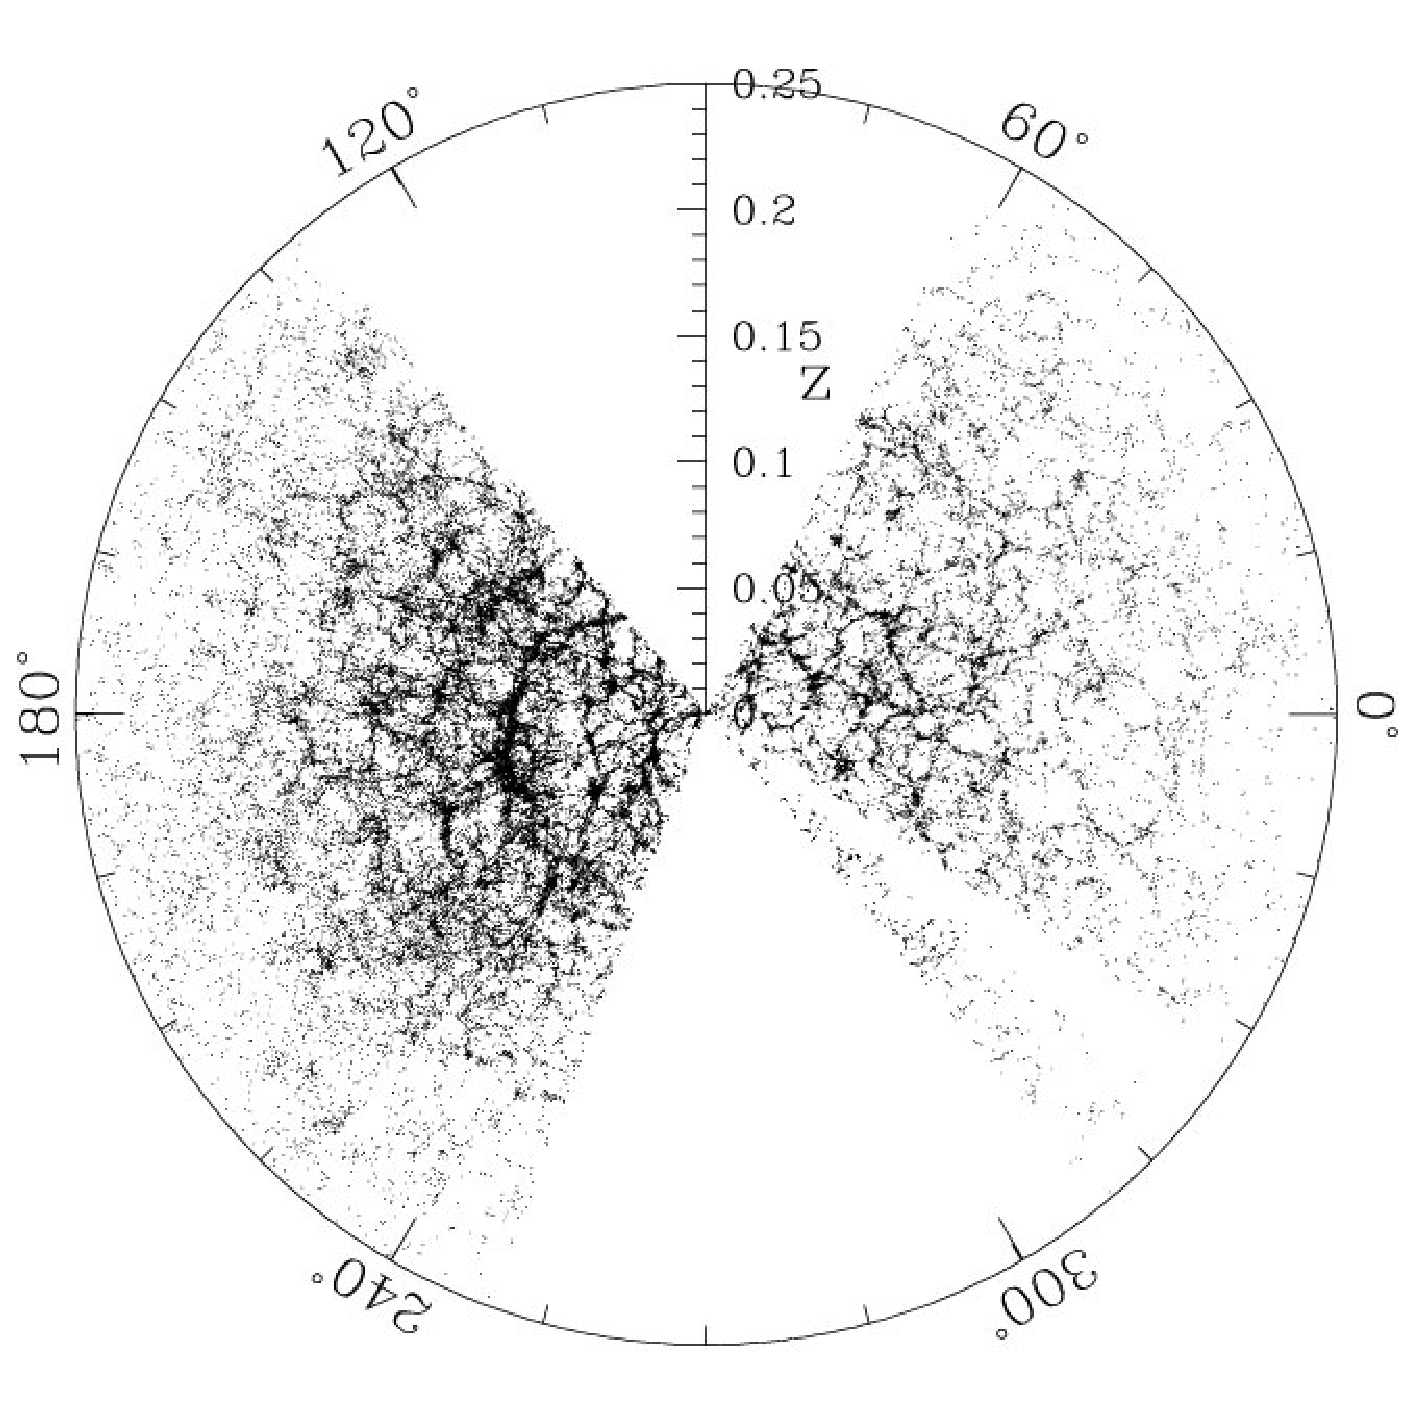
\includegraphics[height=7.5cm]{SDSS.eps}
        \caption{SDSS Spectroscopic Survey Shows Spongy Distribution of Galaxies in the Universe.[source: web$^2$]}\label{SDSS}
        %http://www.fnal.gov/pub/today/archive/archive_2005/today05-05-04.html
 \end{center}  
\end{figure}
\noindent During its first phase operations, 2000-2005, the SDSS imaged more than 8000 square degrees of the sky in five optical bandpasses, and it obtained spectra of galaxies and quasars selected from 5700 square degrees of that imaging. The seventh data relese DR7 imaging data covers about 8423 square degree of  legacy sky and 3240 square degrees fo SEGUE sky. DR7 includes more than 350 million celestial objects and spectra of 930000 galaxies,120,000 quasars and 460,000 stars.\\\\
One of the burning question of the modern astronomy is the problem of origin of angular momentum of the galaxies during their formation. It is interesting and challenging problem to cosmology as well.
%\subsubsection{Primodial Vorticity model:}
%This moel predicts that the spin vectors of galaxies are distributed perpendicular to the cluster plane. The primordial vorticity is called top-down scenario. Sometimes it is also called turbulence model. In the turbulence scenario, an initial large-scale vorted in the protocluste with intinsic vortex is formted and this vorted is fragmented into severl pieces with form teh bsis for the protogalaxies and the galaxies later on.So, the galactic spin vectors are thought to be parallel among themselves and perpendicular to the plane of the cluster.
%
%Ozernoy (1971, 1978) proposes that galaxies form from high-density regions behind the shocks produced by turbulence. According to the primordial vorticity theory, the presence of large chaotic velocities generates turbulence, which, in turn, produces density and pressure fluctuations.
%
%Density fluctuations on the scale of clusters of galaxies could be gravitationally bound, but galactic mass fluctuations are always unbound. Galaxies form when unbound galactic mass eddies, expanding faster than their bound cluster background. So forming galaxies collide with each other as clusters start to recollapse. These collisions produce shocks and high-density proto-galaxies at the eddy interfaces. As clusters recollapse, the system of galaxies undergoes a violent collective relaxation.
%
%
%\subsubsection{Pancake Model}
%The pancake model was first proposed in the 1970s by Yakob B. Zel'dovich at the Institute of Applied Mathematics in Moscow.
%
%The pancake model predicts that the spin vectors of galaxies tend to lie within the cluster plane. In the pancake scenario, formation of clusters took place first and it was followed by their fragmentation into galaxies due to adiabatic fluctuations. According to the non-linear gravitational instability theory, a growth of small inhomogeneities leads to the formation of thin, dense, and gaseous condensations that are called `pancakes'. These condensations are compressed and heated to high temperatures by shock waves causing them to quickly fragment into gas clouds. The later clumping of these clouds results in the formation of galaxies and their clusters.
%
%Thermal, hydrodynamic, and gravitational instabilities arise during the course of evolution. It leads to the fragmentation of gaseous proto-clusters and, subsequently, clustering of galaxies takes place. The pancake scheme follows three simultaneous processes: first, gas cools and new clouds of cold gas form; secondly, these clouds cluster to form galaxies; and thirdly, the forming galaxies and, to an extent, single clouds cluster together to form a cluster of galaxies.
%
%\subsubsection{Hierarchy Model}
%According to the hierarchy model, the directions of the spin vectors should be distributed randomly. In hierarchy model, galaxies were first formed and then they obtained their angular momenta by tidal force while they were gathering gravitationally to form a cluster. Those galaxies grow by subsequent merging of proto-galactic condensations or even by merging of already fully formed galaxies. In this scheme, one could imagine that large irregularities like galaxies grew under the influence of gravities from small imperfections in the early universe.
%
%The angular momentum transferred to a developing proto-galaxy by the gravitational interaction of the quadrupole moment of the system with the tidal field of the matter.
Some people found and discussed similarity of spiral galaxies to turbulent eddies and suggested that the primordial turbulence is respbonsible for the formation of galaxies and may be the origin of the rotation of galaxies (Weizacker 1951 , Gamow 1946). But this model fails because primodial turbulence cannot provide the angular momentum to the galaxies for long time as it dissipates (Jones and Peebles 1972, Jones 1973). Also there is another proposal that the galaxies acquire their angular momentum by the tidal torques of neighbouring protogalaxies (Hoyle 1951, Peebles 1969). But it was unable to explain the empirical relation between angular momentum and mass of the galaxy J$\propto M^{\frac{5}{3}}$ (Barres \& Efstahiou 1987). But in the scenario of global rotation of universe (Li 1998), the corollis force in the galactic frames make galaxies to rotate automatically when they form and galaxies get angular momentum from global rotation of universe due to conservation of angular momentum. So, galaxies rotate because universe rotate.
\section{Theoretical Consideration}
Li explained the empirical relation taking the help of Raychaudhari equation (Ciufolini \& Wheeler 1995) and Einstein field equation (Weinberg 1972).
\subsection{Raychaudhari Equation}
To study the properties of the rotating cosmological model we must define some of the terms like volume scalar expansion, shear tensor and rotation tensor. Raychauduri equation is the connection between these and Ricci curvature tensor.\\\\
Let us consider a ideal fluid whose four velocity $u^\alpha=\frac{dx^\alpha}{ds}$, where $s$ is the parameter of arc length and $x^\alpha\equiv x^\alpha(s)$. And four velocity satisfies the equation
\begin{equation}\label{g_ab}
g_{\alpha\beta}u^\alpha u^\beta=-1
\end{equation}
We can decompose any vector to time like component and space like components by applying a time projection tensor ($-u_\alpha u_\beta$) and space projection tensor $h_{\alpha\beta}=g_{\alpha\beta}+u_\alpha u_\beta$\\
Here,
\begin{eqnarray}\label{projection_time_space}
P_t(v^\alpha)&=&-u_\alpha u_\beta v^\beta\\
P_\Sigma(v^\alpha)&=&h_{\alpha\beta}v^\beta
\end{eqnarray}
Now the length element is given by,
\begin{eqnarray*}
ds^2&=&g_{\alpha\beta} dx^\alpha dx^\beta\\
&=&(h_{\alpha\beta} -u_\alpha u_\beta)dx^\alpha dx^\beta
\end{eqnarray*}
\begin{equation}
ds^2=h_{\alpha\beta}dx^\alpha dx^\beta -u_\alpha u_\beta dx^\alpha dx^\beta
\end{equation}
Let us consider, an observer in $x^\alpha$ which is comoving with the fluid particle with four velocity $u_\alpha$ measures two events $x^\alpha$ and $x^\alpha+dx^\alpha$ at space interval $dl=(h_{\alpha\beta}dx^\alpha dx^\beta)^\frac{1}{2}$ and time interval $d\tau=(u_\alpha u_\beta dx^\alpha dx^\beta)^\frac{1}{2}$\\\\
\textbf{Some properties of $h_{\alpha\beta}$:}
\begin{equation}
\begin{aligned}
h_{\alpha\beta}u^\beta&=&0\hspace{1cm}h_{\alpha\beta}\dot{u}^\beta=h_{\alpha\beta}\underbrace{u^\beta_{;\sigma}u^\sigma}_{\mbox{$a^\beta$}}=h_{\alpha\beta}a^\beta=a_\alpha\\
h^{\alpha\beta}h_{\beta\gamma}&=&h_{\gamma}^{\alpha}\hspace*{1cm} h_{\alpha}^\alpha =3
\end{aligned}
\end{equation}
where $a^\alpha$ is four accleration of fluid particles.\\
Now decomposing $u_{\alpha ;\beta}$ into space like and time like components using projection tensors
\begin{eqnarray*}
u_{\alpha ;\beta}&=& u_{\mu ;\nu}g^\mu_\nu g^\nu_\beta\\
&=& u_{\mu ;\nu}(h^\mu_\alpha-u^\mu u_\alpha)(h^\nu_\beta-u^\nu u_\beta)\\
&=& u_{\mu;\nu}h^\mu_\alpha h\nu_\beta -u_{\alpha;\nu} u^\nu u_\beta
\end{eqnarray*}\\
So the time and space component of  $u_{\alpha ;\beta}$ is given
\begin{equation}\label{u_a_b}
u_{\alpha ;\beta}=u_{\mu;\nu}h^\mu_\alpha h\nu_\beta -u_{\alpha;\nu} u^\nu u_\beta
\end{equation}
Let us introduce three quantities that helps to describe rotating cosmological model:
\begin{itemize}
\item The scalar $\Phi$ of volume expansion\begin{equation}
\Phi=u^\alpha_{;\alpha}
\end{equation}
\item Traceless symmetric tensor of shear:
\begin{equation}
\sigma_{\alpha\beta}=\left[u_{(\mu;\nu)}-\frac{1}{3}\Phi h_{\mu\nu}\right]h^\mu_\alpha h^\nu_\beta$$
\end{equation}
\item The anti-symmetric tensor of vorticity:
\begin{equation}
\omega_{\alpha\beta}=u_{[\mu;\nu]}h^\mu_\alpha h^\nu_\beta
\end{equation}
\end{itemize}
where; $$u_{(\mu;\nu)}=\frac{1}{2}\left(u_{\mu;\nu}-u_{\nu;\mu}\right)$$
$$u_{[\mu;\nu]}=\frac{1}{2}\left(u_{\mu;\nu}+u_{\nu;\mu}\right)$$
Note: \\$a^\beta u_\beta=\sigma_{\alpha\beta}u^{\beta}=\omega_{\alpha\beta}u^{\beta}=0$
\\\\
Using the defined quantities $\Phi$, $\omega_{\alpha\beta}$ and $\sigma_{\alpha\beta}$ we can write \eqref{u_a_b} as,
\begin{equation}\label{phi_sig_ome}
u_{\alpha ;\beta}=\sigma_{\alpha\beta}+\omega_{\alpha\beta}+\frac{1}{3}\Phi h_{\alpha\beta}-a_\alpha a_\beta
\end{equation}
In the above expression $\Phi$, $\omega_{\alpha\beta}$ and $\sigma_{\alpha\beta}$ represents the decompositon of space-space projection of $u_{\alpha ;\beta}$ into trace of symmetric part, antisymmetric part and symmetric traceless part.\\\\
In general, the scalar of expansion $\Phi$ repesents the fractional rate of volume expansion of local ensemble of fluid particles, the shear tensor $\sigma_{\alpha\beta}$ represents the distortion in the generic local fluid ensemble at constant volume and the vorticity tensor $\omega_{\alpha\beta}$ represents the rotation of the generic local ensemble of fluid particles with respect to gyroscope.\\\\
From the tensor analysis we have;
\begin{equation}\label{riemann}
u_{;\mu;\nu}^\alpha-u_{;\nu;\mu}^\alpha=R^\alpha_{\sigma\nu\mu}u^\sigma
\end{equation}
Contracting $\alpha$ and $\nu$ in \eqref{riemann} and multiplying with $u^\mu$ we get;
\begin{equation}\label{R}
u_{;\mu;\alpha}^\alpha u^{\mu}-u^{\alpha}_{;\alpha;\mu}u^{\mu}=R_{\sigma\mu}u^{\sigma}u^{\mu}
\end{equation}
From \eqref{phi_sig_ome} and \eqref{R} we get;
\begin{equation}\label{Raychudhari_0}
\dot{\Phi}-\dot{u}^\alpha_{;\alpha}+2(\sigma^2-\omega^2)+\frac{1}{3}\Phi^2 =-R_{\alpha\beta}u^\alpha u^\beta
\end{equation}
where $\dot{A}^\beta=A^\beta_{;\sigma}u^\sigma$, $\sigma^2=\frac{1}{2}\sigma_{\alpha\beta}\sigma^{\alpha\beta}$, $\omega^2=\frac{1}{2}\omega_{\alpha\beta}\omega^{\alpha\beta}$ and $R_{\alpha\beta}$ is the Ricci Tensor.\\\\
Einstein field equation is given by
\begin{equation}\label{eins}
R_{\mu\nu}-\frac{1}{2} R g_{\mu\nu}= 8\pi T_{\mu\nu}
\end{equation}
Since we are considering perfect fluid the stress energy tensor of the fluid is
\begin{equation}\label{stess}
T_{\mu\nu}=(\rho+p)u_\mu u_\nu -pg_{\mu\nu}
\end{equation}
where $\rho$ and $p$ is the density and pressure of the perfect fluid.
From \eqref{eins} and \eqref{stess} we can find;
\begin{equation}\label{Rab_p_rho}
R_{\mu\nu}u^\mu u^\nu=4\pi(\rho +3p)
\end{equation}
Using \eqref{Rab_p_rho} in \eqref{Raychudhari_0} we get Raychaudhuri equation
\begin{equation}\label{Raychaudhuri}
\dot{\Phi}+\frac{1}{3}\Phi^2+2(\sigma^2-\omega^2)-a^\alpha_{;\alpha}=-4\pi(\rho +3p)
\end{equation}
When particle follows geodesic $a^\alpha=0$. So,
\begin{equation}\label{dust}
\dot{\Phi}+\frac{1}{3}\Phi^2+2(\sigma^2-\omega^2)=-4\pi(\rho +3p)
\end{equation}
From Robertson-Walker (R-W) metric and defination of $\Phi$ we have,
\begin{equation}
\frac{\Phi(t)}{3}=\frac{\dot{R(t)}}{R}=H
\end{equation}
The conservation of energy and momentum (Ellis 1973) gives;
\begin{equation}
\dot{\rho}=-(\rho+p)\Phi\quad\quad\quad \omega\rho a^5= \text{constant}
\end{equation}
We know form R-W metric, for dust $\rho_d\propto a^{-3} $and for radiation $\rho_r\propto a^{-4}$. So, $\omega_d\propto a^{-2}$ and $\omega_r\propto a^{-1}$. But the shear $\sigma$ falls off as $\sigma \propto a^{-3}$\\\\
For dust fluid $a^\alpha=0$, since it follows the geodesic and neglecting the shear term as it is assumed to be small. Then the first integral of \eqref{dust} gives
\begin{eqnarray*}
\dot{\Phi}+\frac{1}{3}\Phi^2-2(\omega^2)&=&-4\pi(\rho +3p)\\
\dot{\Phi}+\frac{1}{3}\Phi^2-2(\omega^2)&=&-4\pi(\rho)\quad\text{(p=0 for dust)}\\
\end{eqnarray*}
And \begin{equation}\frac{\Phi}{3}=H=\frac{\dot{a}}{a}\end{equation} Then, the first integral gives;
\begin{equation}\label{RW_r}
H^2=\frac{8\pi}{3} G\rho-\frac{2}{3}\omega^2-\frac{k}{a^2}
\end{equation}
where k is the integration constant and its value can be +1, 0, -1 by rescaling.\\
We can see \eqref{RW_r} is same as explained by R-W metric adding a centrifugal term due to rotation of the universe.
\subsection{Derivation of Empirical Formula $J\propto M^\frac{2}{3}$}
Let us consider formation of galaxies in rotating and expanding universe. At some early epoch there is density fluctuation in a region then the expansion around the region began to increasily decelerated.\\\\
Let us assume the density fluctuation be spherically symmetric. The region containing the proto-galaxy or matter which will turn galaxy in future is sphere (approximately due to the spherically symmetric density fluctuation).\\\\
Let at that epoch angular momentum relative to the gyroscopic frame be
\begin{equation}\label{J-i}
J_i=\frac{2}{5}M r_i^2 \omega_i
\end{equation}
where $M$ is the mass of the proto galaxies, $r_i$  is the radius of the proto-galaxy and $\omega_i$ is the angular velocity of the universe.\\\\
Again, we can also define a local frame called galactic frame axis which corotate with the global rotation of universe and its origin is fixed at galactic center. This is the frame with which the measurement is taken in real life.\\\\
After the formation of the galaxy, it rotates relative to the galactic frames which is caused by the corollis force or conservation of the angular momentum. At any epoch after the galaxy has formed, its angular momentum relative to the gyroscopic frame is given by
\begin{equation}\label{J-f}
J_f=J+\beta M r_f^2 \omega_f
\end{equation}
where $\omega_f$ is angular velocity of universe at present, $\beta$ is the parameter that depends on the distribution of mass in galaxy, $r_f$ radius of the galaxy at present and $J$ is the angular momentum of the galaxy relative to the galactic frame.\\\\
Also we know that,
\begin{equation}\label{om_rh_m}
\begin{aligned}
\omega_i=\omega_0(1+z_i)^2\\
\rho_d=\rho_{d0}(1+z_i)^3\\
M=\frac{4}{3}\pi\rho_{di}r_i^3
\end{aligned}
\end{equation}
From \eqref{J-i}, \eqref{J-f}, \eqref{om_rh_m} and using law of conservation of angular momentum we get,
\begin{eqnarray*}
J_i&=&J_f\\
\frac{2}{3}M r_i^2 \omega_i &=&  J+\beta M r_f^2 \omega_f\\
\end{eqnarray*}
Finally,
\begin{equation}\label{Jexp}
J=\frac{2}{5}\left(\frac{3}{4\pi\rho_{d0}}\right)^\frac{2}{3}\omega_0 M^\frac{5}{3}-\beta r_f^2(1+z_f)\omega_0 M
\end{equation}
For $z_f$ not too large than 1, second term in \eqref{Jexp} is sufficiently small compared to first term so
\begin{gather*}
J\simeq k M^\frac{5}{3}\\
\text{where} \quad k=\frac{2}{5}\left(\frac{3}{4\pi\rho_{d0}}\right)^\frac{2}{3}\omega_0
\end{gather*}
and this explains the observed empirical relation $J\propto M^\frac{5}{3}$
\subsection{Limiting Value of Angular Momentum}
Minimizing \eqref{Jexp} with respect to M we get,
\begin{eqnarray*}
\frac{dJ}{dM}\rfloor_{M_{min}}&=&0\\
&=&\frac{d}{dM}\left(k M^\frac{5}{3}-l M\right)\rfloor_{M_{min}}\quad \text{where $l=\beta r_f^2(1+z_f)^2\omega_0$}\\
&=&k\frac{5}{3}M_{min}^{\frac{2}{3}}-l
\end{eqnarray*}
\begin{equation}
M_{min}=\left(\frac{3l}{5k}\right)^{\frac{3}{2}}=1.95 r_f^3 (1+z_f)^3 \rho_{d0}
\end{equation}
Hence the mininum angular momentum of a galaxy corresponds to the value of mass $1.95 r_f^3 (1+z_f)^3 \rho_{d0}$

\subsection{Zero Angular Momentum}
From \eqref{Jexp} we get,
\begin{eqnarray*}
J&=&0\\
 \text{or, }k M^\frac{5}{3}&=&lM\\
 \therefore \quad\quad M=\left(\frac{l}{k}\right)^\frac{3}{2}
 \end{eqnarray*}
 
\noindent Hence, the mass corresponding to the 0 angular momentum of galaxy is  $M_0\simeq 2.15 M_{min}$. It is easy to observe that for less and more massive structure predicts $\mid J\mid \neq 0$.\\\\
Till here it was concluded that the galaxy obtained its angular momentum due to the global rotation of the universe. So, one may expect that the spin of galaxies should not distribute in sky randomly, there should be a dipole anisotropy and such kind of anisotropy in the distribution of the spin of galaxies have been found at different levels. Here spherical symmetry is considered but the distribution of galaxy is quiet complicated and moment of inertia is complex so the angular momentum is different from the direction of angular velocity.\\\\
When proto-galaxy rotates and expands together with universe the angular velocity is equal to the global rotation of the universe in both magnitude and direction. The rotation of the universe makes the angular momentum of the protogalaxy which is not alligned with the angular velocity with a fixed direction to precesss about axis of rotation. The magnitude of angular momentum is constant during precission. When the proto-galaxies become separated from the global rotation and expansion of the universe and begins to collapse to form galaxies and the interaction with the surrounding should become more and more weak and eventually negligible. Its angular momentum is constant in both magnitude and direction. It should be determined by the shape of the proto-galaxy and the time when proto-galaxy becomes an isolated system. Its distribution can be expected  almost random instead of strong dipole distribution. As the galaxy evolves the dissipation process inside it causes the components of angular velocity perpendicular to the angular momentum to vanish gradually, eventually the galaxy rotates about the direction of angular momentum.
%\end{document}

%------------------------------------------------------
% Database according to Huang Lee and their methods for
%prediction of the rotating clusters
%------------------------------------------------------
\chapter{Database}

\section{Hwang \& Lee (2007): Database of Rotating Cluster}
Hwang and Lee used redshift and position angle of galaxies to estimate the ratio of cluster rotation amplitude to dispersion and the velocity gradient across the clusters. They took 899 Abell clusters as their sample clusters.\\\\
Methods for identification of the rotating cluster candidates:
\begin{itemize}
\item To select member galaxies in target cluster they used \textquoteleft shifting gapper\textquoteright\,\, by Fadda et al. (1996). They selected 56 clusters in which the number of the galaxies is greater than or equal to 40.
\item To investigate the global rotation property of galaxy the observed radial velocity $v_p$ of the cluster galaxies is fitted with function of position angle $$v_p(\Theta)=v_{sys}+v_{rot}\;sin(\Theta-\Theta_0)$$ where $\Theta$ is projected position angle of galaxy relative to the cluster center (measured from north east), $\Theta_0$ is the projected postion angle of the rotation axis of the cluster, $v_{rot}$ is the systemic velocity of the galaxy clusters.\\\\
Similarly, the effect of global rotation of galaxy clusters also can appear as velocity gradient. They fit the observed radial velocity gradient of the cluster galaxies with a function of a position in the plane of sky.
$$
	v_p(x,y)=v_{sys}+\frac{\partial v}{\partial X}X+\frac{\partial v}{\partial Y}Y
$$ where $X$ and $Y$  are clusteric centric distance in the direction of right ascession and declination respectively. They fitted the observed radial velocities of cluster galaxies with $v_{sys}$ as a fixed value of the mean radial velocity of the cluster galaxies.\\\\
A plot of velocity dispersion of galaxy cluster as a function of $\frac{|v_{rot}|}{\sigma_p}$ and as a function of $\frac{dv}{dR}=\sqrt{\left(\frac{dv}{dx}\right)^2+\left(\frac{dv}{dy}\right)^2}$ was drawn. The rotating cluster has large ratio of the absolute velocity dispersion and has large velocity gradient across the cluster. So, among 56 clusters they selected 12 rotating clusters whose $|\frac{v_{rot}}{\sigma_p}|>0.53$ and $\frac{dv}{dR}>380$ km\,s$^{-1}$\,Mpc$^{-1}$.
\end{itemize}

\begin{table*}
\caption[]{Database of three rotating clusters. First three columns
list the Abell name and positions of the cluster center as given
in ACO catalog (Abell et al. 1989). The next three columns give
cluster morphology (BM type classification, Bautz \& Morgan 1970),
mean radial velocity ($cz$ km\,s$^{-1}$) of the cluster and velocity dispersion
($\sigma_{\rm P}$ km\,s$^{-1}$) as given in Hwang \& Lee  (2007). The last
three columns give the number (N) of galaxies with known
diameters,  cluster diameters (arcmin) (Abell et al. 1989) and X-ray
luminosity (10$^{44}$\,erg\,cm$^{-2}$\,s$^{-1}$) (Ledlow et al. 2003, Bohringer et al. 2004).}
$$
 \begin{array}{lllllllll}
            \hline
            \noalign{\smallskip}
            $Cluster$  &  $R.A.$     & $Dec.$     &  $BM-type$ &  $cz$  &  \sigma_{\rm p}     &  $N$  &  $$a$$ & L_{x}\\
             \noalign{\smallskip}
            \hline
            \noalign{\smallskip}
            A1139    &   10^{\rm h}58^{\rm m}10.39^{\rm s}   &   01^{\circ}35'11.0'' &   $III$    &   11\,849   &   491    &   121 & 70  &  0.09  \\
            A2162    &   16^{\rm h}12^{\rm m}30.00^{\rm s}   &   29^{\circ}32'23.0'' &   $II-III$ &   9\,653    &   416    &   41  & 356  &  0.01  \\
            A2366    &   21^{\rm h}42^{\rm m}50.41^{\rm s}   &   06^{\circ}52'15.0'' &   $I-II$   &   15\,914   &   604    &   41  & 40  &  0.05  \\
            \noalign{\smallskip}
            \hline
         \end{array}
     $$
\end{table*}


\begin{figure}[H]
\centering 
\centering
   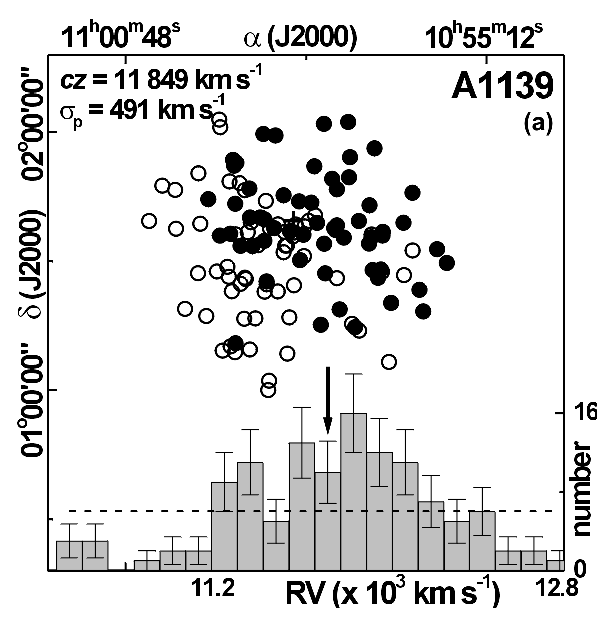
\includegraphics[height=6.0cm]{fig3a.eps}
   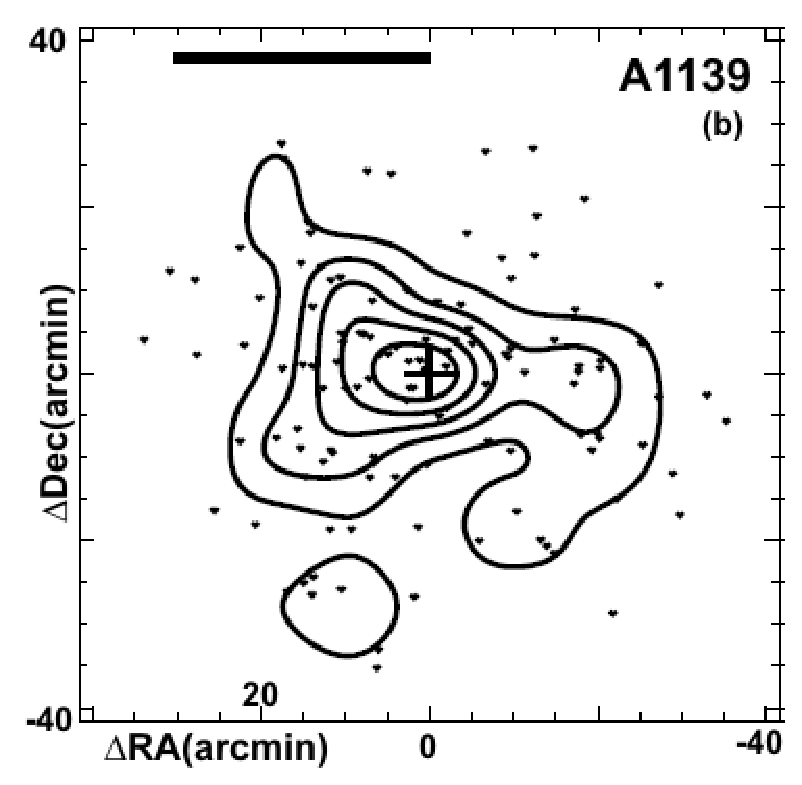
\includegraphics[height=6.0cm]{fig3b.eps}\\
   \includegraphics[height=6.5cm]{gal_a1139.eps}
   \includegraphics[height=6.5cm]{sup_a1139.eps}
   \caption{(a) All sky distribution of galaxies in the cluster A1139. The solid (hollow) circle represents the galaxies that have radial velocity less (greater) than
      the mean radial velocity ($cz$) of the cluster. The histogram showing RV distribution of galaxies can be seen.
      The dashed line and an arrow represent the average distribution and the cluster mean radial velocity ($cz$).
      (b) Galaxy number density map. The member galaxies are represented by dots, and the number density contours are overlaid.
      The cross indicates the cluster center, and the thick horizontal bar represents the physical size of 1 Mpc.
    (c) All sky distribution of the galaxies in galactic coordinate system. (d) All sky distribution of galaxies in the Supergalactic coordinate system.}
\end{figure}
\begin{figure}[H]
\centering
      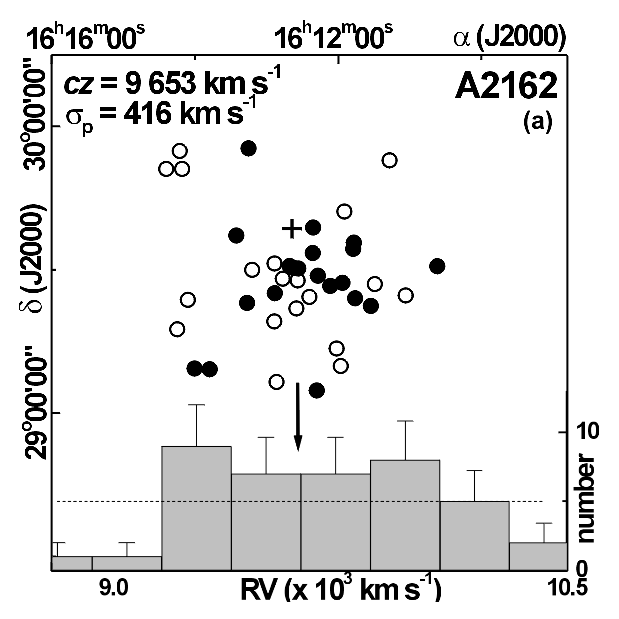
\includegraphics[height=6.0cm]{fig5a.eps}
   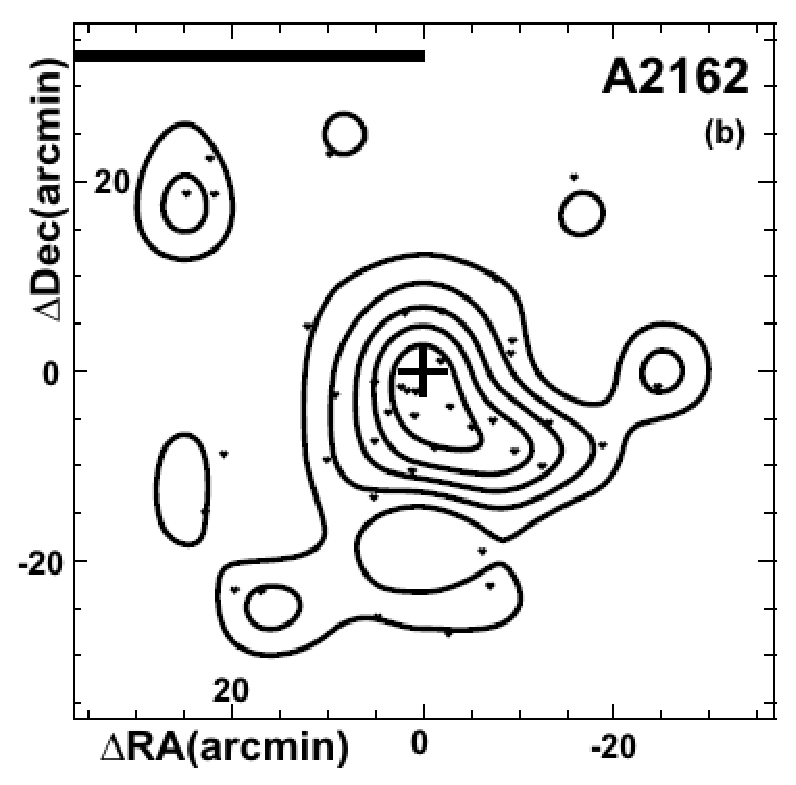
\includegraphics[height=6.0cm]{fig5b.eps}\\
    \includegraphics[height=6.5cm]{gal_a2162.eps}
   \includegraphics[height=6.5cm]{sup_a2162.eps}
   \caption{(a) All sky distribution of galaxies in the cluster A2162. The solid (hollow) circle represents the galaxies that have radial velocity less (greater) than
      the mean radial velocity ($cz$) of the cluster. The histogram showing RV distribution of galaxies can be seen.
      The dashed line and an arrow represent the average distribution and the cluster mean radial velocity ($cz$).
      (b) Galaxy number density map. The member galaxies are represented by dots, and the number density contours are overlaid.
      The cross indicates the cluster center, and the thick horizontal bar represents the physical size of 1 Mpc.
    (c) All sky distribution of the galaxies in galactic coordinate system. (d) All sky distribution of galaxies in the Supergalactic coordinate system.}
\end{figure}
\begin{figure}[H]
\centering
   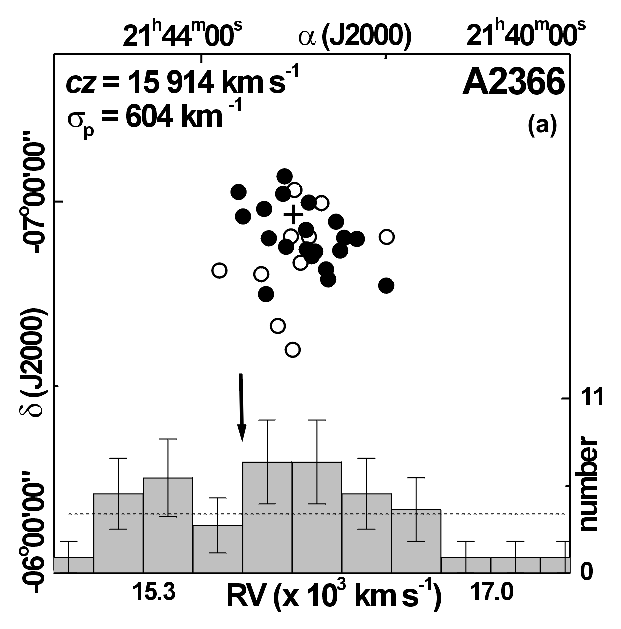
\includegraphics[height=6.1cm]{fig7a.eps}
   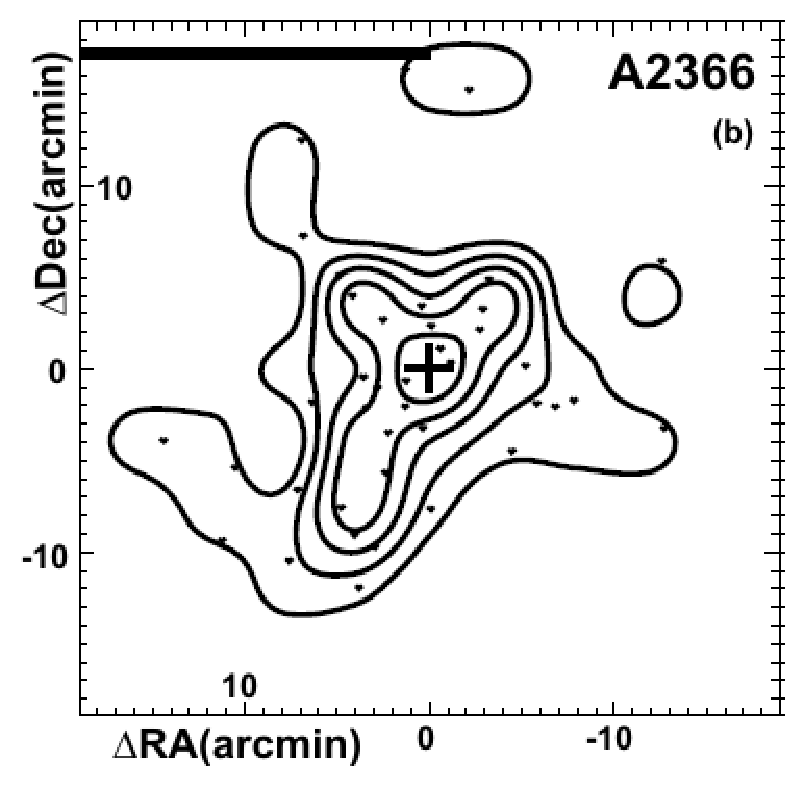
\includegraphics[height=6.0cm]{fig7b.eps}\\
    \includegraphics[height=6.5cm]{gal_a2366.eps}
   \includegraphics[height=6.5cm]{sup_a2366.eps}
   \caption{(a) All sky distribution of galaxies in the cluster A2366. The solid (hollow) circle represents the galaxies that have radial velocity less (greater) than
      the mean radial velocity ($cz$) of the cluster. The histogram showing RV distribution of galaxies can be seen.
      The dashed line and an arrow represent the average distribution and the cluster mean radial velocity ($cz$).
      (b) Galaxy number density map. The member galaxies are represented by dots, and the number density contours are overlaid.
      The cross indicates the cluster center, and the thick horizontal bar represents the physical size of 1 Mpc.
    (c) All sky distribution of the galaxies in galactic coordinate system. (d) All sky distribution of galaxies in the Supergalactic coordinate system.}
\end{figure}



%------------------------------------------------------
 %methods: PA-inclination method, Simulation procedure and about the Statistics
 % matlab code
%------------------------------------------------------
\chapter{Methods of Analysis}

\section{Methodology}
\subsection{Transformation of Coordinates}
The data that we have received was in equatorial coordinate system but we want it to be analysed in the galactic and Supergalactic coordinate system so we used the code written in python for the web scrapping from NED calculator.
\subsection{Transformtion From 2-D to 3-D}
The primary data that we obtained contains only longitude, latitude, major axis, minor axis and the position angle. These are  the information about the 2-D projection of the galaxies on the surface of the celestial sphere. But our goal is to study the orientation of the spin vectors in the space and this requires the 3-D information about the galaxies. So, we used `PA-inclination' method as proposed by Flin \& Godlowski (1986) in order to convert two dimensional given parameters to three dimensional parameters. The formula to obtain the three dimensional information about the spin vector of the galaxies is given in Appendix \ref{God}. The equation used for transformation are,
\begin{equation}\label{goldwski}
\begin{array}{l}
\sin \theta = -\cos i\sin \delta \pm \sin i\sin P\cos \delta;\\
\\
\sin \phi = \frac{- \cos i\cos \delta\sin \alpha + \sin i(\mp \sin P \sin \delta\sin \alpha \mp \cos P\cos \alpha)}{\cos \theta};\\
\\
\cos \phi = \frac{- \cos i\cos \delta\cos \alpha + \sin i(\mp \sin P \sin \delta\cos \alpha \pm \cos P\sin \alpha)}{\cos \theta}.\\
\end{array}
\end{equation}
\\
Here, $i$, $\delta$, $\alpha$ and $P$ represent the inclination
angle, declination, right ascension and position angles (angle made by the major axis with celestial north pole measured from north-east-south)
respectively.
\\
\\
The inclination angle $i$, is the angle between the normal to the
galaxy plane and the observer's line-of-sight and can be estimated
with the Holmberg's (1946) formula. (Appendix \ref{holm})
\begin{equation}
\begin{array}{l}
\cos^2 i = \frac{q^2 - q*^2}{1 - q*^2}
\end{array}
\end{equation}
Here, q and q* represent the measured axial ratio ($b$/$a$) and
the intrinsic flatness of the galaxy respectively. The intrinsic
flatness of a disk galaxy depends on the morphological type. Here we have used q*=0.2 which means if we go on increasing the opening angle of the disk it can be converted into sphere in 5-folds.
\subsection{Expected Distribution: Numerical Simulation}
Aryal \& Saurer (2002) studied the effects of various types of selections in galaxy orientation study and concluded that any selections on the data may cause severe changes in the shapes of the expected isotropic distribution curves. Their method has been applied by several authors in galaxy orientation studies. Our galaxy samples are the members of the clusters which are located in a limited regions of the sky. Thus, it is of importance to remove both the positional and the inclination effects. Three kinds of selection effects are noticed in our database: (1) inhomogeneous distribution of position of galaxies, (2) lack of knowledge of position angles of nearly face-on galaxies and (3) lack of edge-on galaxies. These selection effects are removed and the expected isotropic distribution curves are determined using the numerical simulation methods as proposed by Aryal \& Saurer (2000). For this, a true spatial distribution of the galaxy rotation axis is assumed to be isotropic. Then, due to the projection effects, $i$ can be distributed $\propto\,sin\,i$, latitude can be distributed $\propto\,cos\,B$, the variables longitude ($L$) and position angle can be distributed randomly, and formula \eqref{goldwski} is used to simulate the corresponding distribution of $\theta$ and $\phi$. The simulation procedure is described in Aryal \& Saurer (2004).

\subsection{Octave Code}
We have developed a code named `GOBAD1.0' which offers random simulations and all calculations including statistics given in papers Holmberg (1946), Flin \& Godlowski (1986), Godlowski (1993), Aryal \& Saurer (2000), Press et al. (1992) and Hyanes \& Giovanni (2007) in order to carry out a systematic study of spatial orientation of spin vectors of galaxies in the clusters and Superclusters. This code is in the process of publication in MNRAS. We have used this code in order to study the spatial orientation of galaxies in three rotating clusters in this dissertation. The results of this work is already published in MNRAS (2013).
\subsubsection*{main.m}
\begin{verbatim}
%--------------------------------------------------------------------- 
%  Programmer: Bhattarai H.                                                                         
%	           Central Department Of Physics                   
%              Tribhuvan University                             
%              Kirtipur, Nepal                                  
%----------------------------------------------------------------------

clear all, clc, close all;
%--------------------------------------------------------------------------
'***************************Data loaded************************************'
%--------------------------------------------------------------------------

data=load('data.dat');   
%load data from the destination folder which in .dat format 
%having L,B,P and I in cosecutive columns                
                       
%---------------------------------------------------------------------------   
		'*****************Coordinte transformation ************************'
%---------------------------------------------------------------------------
l=data(:,2);
b=data(:,3);
p=data(:,4);
i=data(:,1);
save('gal_cod.mat','l','b','p','i')    

%---------------------------------------------------------------------------
  '***********************Godlowski_Transformation *********************'
%---------------------------------------------------------------------------
clear all, 
load gal_cod.mat
[theta1,theta2,phi1,phi2]=godlowski_transformation(l,b,p,i); 
 
th=abs([theta1;theta2]');
ph=[phi1;phi2]';

dx_theta=5:10:85;
dx_phi=-80:20:80;
n_theta_bins=max(size(dx_theta));
n_phi_bins=max(size(dx_phi));
figure(1);
clf()
hist(th,dx_theta);
title 'Histogram of theta '
xlabel 'theta'
ylabel '# of galaxies'
xlim([-90,90])
print -dpdf 1_theta_histo.pdf

figure(2);
clf()
hist(ph,dx_phi);
title 'Histogram of phi';
xlabel 'phi';
ylabel '# of galaxies'
xlim([0,90])
print -dpdf 2_phi_histo.pdf

save('godl_trans.mat','th','ph','n_theta_bins','n_phi_bins');

%--------------------------------------------------------------------
'**************************Histogram:****************************'
%--------------------------------------------------------------------
clear all; close all, 
load gal_cod.mat

%------------------ HISTOGRAM FOR L -------------------------------------
[l_n,l_data_in_bin,l_binsize,l_bin_start,l_bin_end]=histo_galactic(l,2);
save ('hist_l.mat','l_n','l_data_in_bin','l_binsize','l_bin_start','l_bin_end')
figure(3);
clf()
hist(l,l_n);
xlabel 'l'
ylabel '# galaxies'
title 'Histogram of l'
print -dpdf 3_hist_l_data.pdf

%----------------- HISTOGRAM FOR B ----------------------------------------
[b_n,b_data_in_bin,b_binsize,b_bin_start,b_bin_end]=histo_galactic(b,2);
save ('hist_b.mat','b_n','b_data_in_bin','b_binsize','b_bin_start','b_bin_end')
figure(4);
clf()
hist(b,b_n);
xlabel 'b'
ylabel '# galaxies'
title 'Histogram of b'
print -dpdf 4_hist_b_data.pdf

%---------------- HISTOGRAM FOR P ----------------------------------------
[p_n,p_data_in_bin,p_binsize,p_bin_start,p_bin_end]=histo_galactic(p,2);
save ('hist_p.mat','p_n','p_data_in_bin','p_binsize','p_bin_start','p_bin_end')
figure(5);
clf()
hist(p,p_n);
xlabel 'p'
ylabel '# galaxies'
title 'Histogram of p'
print -dpdf 5_hist_p_data.pdf

%--------------- HISTOGRAM OF I ---------------------------------------------
[i_n,i_data_in_bin,i_binsize,i_bin_start,i_bin_end]=histo_galactic(i,2);
save ('hist_i.mat','i_n','i_data_in_bin','i_binsize','i_bin_start','i_bin_end')
figure(6);
clf()
hist(i,i_n);
xlabel 'i'
ylabel '# galaxies'
title 'Histogram of i'
print -dpdf 6_hist_i_data.pdf

%-----------------------------------------------------------------------------
'***********************VIRTUAL GALAXIES SIMULAITON********************'
%-----------------------------------------------------------------------------
'*******************Virtual galaxies simulated for L***********************'
clear all; close all; 
load hist_l.mat
[sim_l,total_data_l]=simulation(10^5,l_n,l_data_in_bin,l_bin_start,l_binsize);
save ('virtual_l.mat','sim_l','total_data_l');

%----------------------------------------------------------------------------
'*******************Virtual galaxies simulated for B**********************'
clear all,close all;
load hist_b.mat
[sim_b,total_data_b]=simulation(10^5,b_n,b_data_in_bin,b_bin_start,b_binsize);
save ('virtual_b.mat','sim_b','total_data_b');

%------------------------------------------------------------------------------
'**********************Virtual galaxies simulated for P********************'
clear all,close all;
load hist_p.mat
[sim_p,total_data_p]=simulation(10^5,p_n,p_data_in_bin,p_bin_start,p_binsize);
save ('virtual_p.mat','sim_p','total_data_p');

%------------------------------------------------------------------------------
'*************************Virtual galaxies simulated for i*****************'
clear all,close all;
load hist_i.mat
[sim_i,total_data_i]=simulation(10^5,i_n,i_data_in_bin,i_bin_start,i_binsize);
save ('virtual_i.mat','sim_i','total_data_i');

%-------------------------------------------------------------------------------
'***********Godlowski_Transfomation for virtual galaxies ***************'
%------------------------------------------------------------------------------
clear all,close all;

load virtual_b
load virtual_p
load virtual_l
load virtual_i

min_dim=min([total_data_l,total_data_b,total_data_p,total_data_i]);

[theta_1,theta_2,phi_1,phi_2]=godlowski_transformation(sim_l(1:min_dim)...
,sim_b(1:min_dim),sim_p(1:min_dim),sim_i(1:min_dim));

theta=abs(transpose([theta_1,theta_2]'));
phi=transpose([phi_1,phi_2]');

save('virtual_theta_phi.mat','theta','phi');

%-------------------------------------------------------------------------------
'*************** COMPARING THE SIMULATED VRS REAL DATA ******************'
%-------------------------------------------------------------------------------
clear all,close all

load godl_trans.mat;
load virtual_theta_phi.mat;
dx_theta=5:10:85;
dx_phi=-80:20:80;

theta_data=th;
phi_data=ph;

[n_data_bins_theta,data_bin_cent_theta]=hist(theta_data,dx_theta);
[n_data_bins_phi,data_bin_cent_phi]=hist(phi_data,dx_phi);

[n_simul_bins_theta,simul_bin_cent_theta]=hist(abs(theta),dx_theta);
[n_simul_bins_phi,simul_bin_cent_phi]=hist(phi,dx_phi);

n_simul_bins_phi=n_simul_bins_phi;
n_simul_bins_theta=n_simul_bins_theta/2;
n_data_bins_phi=n_data_bins_phi;
n_data_bins_theta=n_data_bins_theta/2;

n_simul_bins_phi_norm=n_simul_bins_phi*(sum(n_data_bins_phi)...
/sum(n_simul_bins_phi));

n_simul_bins_theta_norm=n_simul_bins_theta*(sum(n_data_bins_theta)...
/sum(n_simul_bins_theta));

dx_theta_l=(linspace(0,90,100));
dx_phi_l=(linspace(-90,90,200));

theta_simul=spline(data_bin_cent_theta,n_simul_bins_theta_norm,dx_theta_l);
phi_simul=spline(data_bin_cent_phi,n_simul_bins_phi_norm,dx_phi_l);
%--------------------------------------------------------------------------------
figure(10);
plot(data_bin_cent_theta,n_data_bins_theta,'oy',data_bin_cent_theta,...
n_simul_bins_theta_norm,'sb',dx_theta_l,theta_simul,'r--');

for i=1:n_theta_bins
    hold on,   
    errorbar(data_bin_cent_theta(i),n_data_bins_theta(i),sqrt(n_data_bins_theta(i)))
end
xlabel 'theta';
ylabel '#';
title 'sim vrs real theta';
print -dpdf 9_sim_vrs_real_theta.pdf;
%--------------------------------------------------------------------------------
figure(11);
plot(data_bin_cent_phi,n_data_bins_phi,'oy',data_bin_cent_phi,...
n_simul_bins_phi_norm,'sb',dx_phi_l,phi_simul,'r--');

for i=1:n_phi_bins
    hold on,   
    errorbar(data_bin_cent_phi(i),n_data_bins_phi(i),sqrt(n_data_bins_phi(i)))
end

xlabel 'phi';
ylabel '#';
title 'sim vrs real phi';
print -dpdf 10_sim_vrs_real_phi.pdf;
%-----------------------------------------------------------------------------------
'*************************STATISTICAL TEST*********************************'
%-----------------------------------------------------------------------------------
[ fourier_coeff_theta,theta_P_greater_delta_1 ]=...
    fourier_test(n_simul_bins_theta_norm,n_data_bins_theta,data_bin_cent_theta)
[ fourier_coeff_phi,phi_P_greater_delta_1 ]=...
    fourier_test(n_simul_bins_phi_norm,n_data_bins_phi,data_bin_cent_phi)

chi_theta=chi2test(n_data_bins_theta,n_simul_bins_theta_norm)
chi_phi=chi2test(n_data_bins_phi,n_simul_bins_phi_norm)
auto_corr_theta=auto_correlation(n_data_bins_theta,n_simul_bins_theta_norm)
auto_corr_phi=auto_correlation(n_data_bins_phi,n_simul_bins_phi_norm)
H_ks_theta=ks_test(th',abs(theta'))
H_ks_phi=ks_test(ph',phi')
H_kv_theta=kv_test(th',abs(theta'))
H_kv_phi=kv_test(ph',phi')
%------------------------------------------------------------------------------------
\end{verbatim}
\pagebreak
\subsubsection*{histo\_galactic.m}
Histo\_galactic.m is the function file which takes the data and minimum number of data that each bin must contain and gives total number of bins, data in each bin, size of bin, bin start positon and bin ending postion as function output.
\begin{verbatim}
function [ n,data_in_bin,binsize,bin_start,bin_end ] =histo_galactic...
( data,min_number )

%HISTOGALACTIC
%   This function determines the no of bins, data in each bin,size of bin,
%   bin start positon and bin end position

a=length(data);
i=a;
c=1;
while c~=0
    n=hist(data,i); 
    c=0;
    for j=1:length(n)
        if (n(j)<min_number)
           c=c+1;
         end         
   end
    i=i-1;
end
n=i+1;
[data_in_bin,h]=hist(data,i+1);
binsize=h(2)-h(1);
bin_start=h(1)-binsize/2;
bin_end=h(length(h))+binsize/2;
end
\end{verbatim}
\subsubsection*{godlwski\_transformation.m}
Godlwski\_transformation.m is the function which implements the \eqref{goldwski} for the calculation of the polar angle ($\theta$) and azumithal angle ($\phi$) of the spin vector of galaxies.
\begin{verbatim}
function [ theta1,theta2,phi1,phi2 ] = godlowski_transformation( l,b,p,i )
%GODLOWSKI_TRANSFOMATION 
% this transformation converts 2-d data to 3-d information of the galaxy
% the input are Latitude, longitude, positional angle and inclination
% the output are theta1,theta2,phi1 and phi2

L=degrad(l);
B=degrad(b);           %converts all the angle in degrees to radian
P=degrad(p);
I=degrad(i);

% delta1 = asin(-cos(i).*sin(B)+ sin(i).*sin(P).*cos(B));	%polar angle
% delta2 = asin(-cos(i).*sin(B)- sin(i).*sin(P).*cos(B));	%polar angle
% 
% eta1 = asin ((-cos(i).*cos(B).*sin(L) + sin(i).*(-sin(P).*sin(B).*sin(L)-
%cos(P).*cos(L)))./cos(delta1));  %azimuthal angle
% eta2 = asin ((-cos(i).*cos(B).*sin(L) + sin(i).*(+sin(P).*sin(B).*sin(L)+
%cos(P).*cos(L)))./cos(delta2));  %azimuthal angle

theta1_rad=asin(-cos(I).*sin(B)+sin(I).*sin(P).*cos(B));
phi1_rad=asin((-cos(I).*cos(B).*sin(L)+sin(I).*(-sin(P).*sin(B).*sin(L)...
    -cos(P).*cos(L)))./cos(theta1_rad));

theta2_rad=asin(-cos(I).*sin(B)-sin(I).*sin(P).*cos(B));
phi2_rad=asin((-cos(I).*cos(B).*sin(L)+sin(I).*(sin(P).*sin(B).*sin(L)...
    +cos(P).*cos(L)))./cos(theta2_rad));

theta1=raddeg(theta1_rad);
theta2=raddeg(theta2_rad);

phi1=raddeg(phi1_rad);
phi2=raddeg(phi2_rad);

\end{verbatim}
\subsubsection*{simulation.m}
Simulation.m is the function that performs the numerical simulation as explained in the section in 4.1.3.
\begin{verbatim}
function [simulated_data,total_data ] = simulation( no_of_galaxies,no_of_bins...
,data_in_bin,bin_start,bins_size )


% SIMULATION[no_of_galaxies,no_of_bins,data_in_bins,bin_start,bin_size]
% THis function helps to eliminate the selection effect of the galaxies by
% doing the simulaiton considering homogenity and isotropy of the universe.

prop=zeros(no_of_bins,1);
for i=1:no_of_bins
    prop(i)=ceil((data_in_bin(i)*no_of_galaxies/(sum(data_in_bin))));
   
end
k=1;

for i=1:no_of_bins
    ran_gal=rand(prop(i),1);
        for j=1:prop(i)
             A(k)  =(bins_size*ran_gal(j,1))+bin_start+(i-1)*bins_size;
             k=k+1;
        end
end
total_data=sum(prop);
rand_pos=randperm(sum(prop)); 
LL=A(rand_pos(:));
simulated_data=LL;
end
\end{verbatim}
\textbf{\large{Statistical Test}}
\subsubsection*{chi2test.m}
Performs the $\chi^2$ test as explained in section \ref{chi}.
\begin{verbatim}
function [ prob ] = chi2test( obs,theo)
%[Prob]= CHI2TEST(OBS,THEO)
%  The above funciton return the probablity that the observed distribution
% is same as the theoretical distribution.

n=max(size(obs));
% to eliminate data where theoretical value is 0
for i=1:n
    if theo(i)<=7 || obs(i)<=7
        theo(i)=1;
        obs(i)=1;
    end
end
 chi2=sum((obs-theo).^2./theo);
 a=(n-1)/2;
 f=@(x)exp(-x).*x.^(a-1);
 p=1/gamma(a)*quad(f,0,chi2/2);
 prob=1-p;
end
\end{verbatim}
\subsubsection*{auto\_correlation.m}
Performs the auto-correlaiton test as explained in section \ref{auto}.
\begin{verbatim}
function [ c_coefficient ] = auto_correlation( obs,theo )
% [CORRELATION_COEFFICIENT]=AUTO_CORRELATION(OBSERVED_NUMBER,THEORETICAL_NUMBER)
%  This funciton calculates the autocorrelation coefficient when observed
% and theoretical number of data  in each bin is passed to the function


n=max(size(obs));
c=0;
for i=1:n-1
    
    if obs(i)<=7 || theo(i)<=7 || obs(i+1)<=7 || theo(i+1)<=7
        d=0;
    else
        d=(obs(i)-theo(i))*(obs(i+1)-theo(i+1))/sqrt(theo(i)*theo(i+1));
    end
    c=c+d;
end
sigma_c=sqrt(n);
c_coefficient=c/sigma_c;  

end
\end{verbatim}
\subsubsection*{fourier\_test.m}
Performs the fourier test as explained in section \ref{fourier}
\begin{verbatim}
function [ first_coefficient,P_greater_delta_1 ]...
    = fourier_test( N_th,N_obs,angles )
%FOURIER_TEST
%This function take the theoretical and observed number of galaxies with 
%their resepective bin anlges and calulates different parameters in fourie
%er test.
angles=degrad(angles);

delta_11=sum((N_obs-N_th).*cos(2*angles))./sum(N_th.*(cos(2*angles).^2));

delta_21=sum((N_obs-N_th).*sin(2*angles))./sum(N_th.*(sin(2*angles).^2));

sigma_11=sqrt(sum(N_th.*(cos(2*angles)).^2));
sigma_21=sqrt(sum(N_th.*(sin(2*angles)).^2));
delta_1=sqrt(delta_11^2+delta_21^2);
a=max(size(N_obs));
P_greater_delta_1=exp(-a/4.0*sum(N_obs)*delta_1^2);
first_coefficient=delta_11/sigma_11;
end
\end{verbatim}
\subsubsection*{ks\_test.m}
Performs the Kolmogorov-Smirnov (K-S) test as explained in section \ref{kstest}.
\begin{verbatim}
function [H] = ks_test(obs,theo )

edges=[-inf;sort([obs;theo]);inf];
count1=histc(obs,edges);
count2=histc(theo,edges);

sumcount1=cumsum(count1)./sum(count1);
sumcount2=cumsum(count2)./sum(count2);

cdf1=sumcount1(1:end-1);
cdf2=sumcount2(1:end-1);

diffcdf=abs(cdf1-cdf2);
n1=length(obs);
n2=length(obs);

n=n1*n2/(n1+n2);
ks=max(diffcdf);

lambda=max((sqrt(n)+0.12+0.11/sqrt(n))*ks,0);
k=(1:101)';
p=2*sum((-k).^(k-1).*exp(-2*lambda*lambda*k.^2));
p=min(max(p,0),1);
alpha=0.05;
H=(alpha>=p);
if H==0
    'Null hypothesis accepted'
else
   'Null hypothesis rejected'
end
end

\end{verbatim}
\subsubsection*{kv\_test.m}
Performs the Kupier-V test as explained in section \ref{kvtest}.
\begin{verbatim}
function [H] = kv_test(obs,theo )
edges=[-inf;sort([obs;theo]);inf];
count1=histc(obs,edges);
count2=histc(theo,edges);

sumcount1=cumsum(count1)./sum(count1);
sumcount2=cumsum(count2)./sum(count2);

cdf1=sumcount1(1:end-1);
cdf2=sumcount2(1:end-1);

diffcdf1=(cdf1-cdf2);
diffcdf2=(cdf2-cdf1);
n1=length(obs);
n2=length(obs);

n=n1*n2/(n1+n2);
d1=max(diffcdf1);
d2=max(diffcdf2);
ks=d1+d2;

lambda=max((sqrt(n)+0.155+0.24/sqrt(n))*ks,0);
k=(1:101)';
p=2*sum((4*k.^2.*lambda.^2-1).*exp(-2*lambda*lambda*k.^2));
p=min(max(p,0),1);
alpha=0.05;
H=(alpha>=p);
if H==0
    'Null hypothesis accepted'
else
   'Null hypothesis rejected'
end
end
\end{verbatim}
\subsubsection*{raddeg.m}
\begin{verbatim}
function [out]=raddeg(in)
% converts radian to degree
out=180/pi.*in;
\end{verbatim}
\subsubsection*{degrad.m}
\begin{verbatim}
function [out]=degrad(in)
%converts degree to radain
out=pi/180.*in;
\end{verbatim}

%------------------------------------------------------
 %Statistical Results: Polar and Azimuthal angle distribution
%------------------------------------------------------

%------------------------------------------------------
\chapter{Result and Discussion}
\section{Literature Review}
\subsection{Abell 2162}
Giacintucci et al. (2013) presented the morphological study and spectral analysis for sample of 13 cD galaxies in rich and poor clusters of galaxies. Their study is based on new high sensitivity Gaint Meterwave Radio Telescope (GMRT) observations at 1.28 GHz, 610 MHz and 235 MHz. The GMRT full resolution image at 235 MHz shows two opposite lobes, with lack of a central compact component at both frequencies. The radio emission is weak and surface brightness is low. A similar double morphology without central component was found also at 1.4 GHz by Owen \& Ledlow (1997). The source has linear size of $\approx$ 90 $\times$ 38 Kpc. They also found that A2162 shows fairly relaxed morphology of the lobes and lack nuclear emission and these features are consistent with the idea that they are aged radio galaxies.\\\\
Liuzzo et al. (2010) presented new VLBI observations at 5GHz of a complete sample of Brightest Cluster Galaxies (BCGs) in Abell Clusters. The detailed discussion about the distribution of the absolute magnitude of BCGs which is not correlated to the dynamic equilibrium of their host-clusters can be found in Hoessel et al. (1980). These galaxies are intimately related to the collapse and formation of clusters: recent models suggest that BCGs must form earlier, and the galaxy merging with the clusters during collapse within a cosmological hierarchy is a visible scenario (Bernardi et al. 2006). The Abell cluster is a low X-ray luminosity clusters (Burns  et al. 1994). Its BCG is NGC6086 is a bright cD galaxy which hosts a double-lobed radio source. In the NVSS image, the total flux density is $\approx$ 108.7 nJy. The radio spectrum and morphology suggests that it is relic galaxy where the core radio activity stopped some time ago.\\\\
Abell 2162 is member of the Hercules super cluster complex (Einasto et al. 2001). The X-ray emission of this nearby cluster of galaxies has been studied by Ledlow et al. (2003) who reported an X-ray luminosity in the 0.5-2.0 keV band of 0.16 $\times 10^{43}$ erg\,s$^{-1}$ based on ROSAT data. The fading radio lobes of B2 1610+29 associated with NGC 6086, the brightest galaxy of the cluster located close to the X-ray peak.\\\\
Donzelli, Muriel, Madrid (2011) derived detailed R band luminosity profiles and light profiles were initially fitted with a Sersic's $R^{\frac{1}{n}}$ model. The effective surface magnitude and central surface magnitude is 20.85 and 22.46 respectively. The effective radius is 7.19 Kpc and n parameter is 3.92.\\\\
Gal et al. (2000) presents photometric redshifts for 431 Abell clusters imaged as part of the Palomar Abell Cluster Optical Survey (PACOS). For this cluster (\textit{g-r}) is 0.43867 and $g_{mean}$ = 20.2053.\\\\
Miller (2001) used the NRAO VAL Sky Survey (NVSS) to identify radio galaxies in eighteen nearby Abell clusters. A2162 contains only four radio galaxies consitent with the cluster at \textit{z} $\approx$ 0.03 whereas six radio galaxies are at \textit{z} $\approx$ 0. The zero point magnitude assumed for POSS II photometry of the cluster is 30.24 and average extinction assumed for POSS II photometry is 0.04. The separation between optical position and radio position as specified in NVSS catalog 29.2 and Radio flux at 1.4 GHz determined directly from the NVSS image 113.4.\\\\
Mahdavi et al. (2001) demonstrated that individual elliptical galaxies and clusters of galaxies form a continuous X-ray luminosity -velocity dispersion($L_X-\sigma$) relation. Their sample of 280 clusters have $L_x\propto\sigma^{4.4}$. For this cluster log$\sigma$ is 2.56$\pm$0.07 km\,s$^{-1}$ and log$L_x$ is 43.32$\pm$0.10 $h_{50}^{-2} $erg\,s$^{-1}$\\\\
Haynes et al. (2004) conducted a study of optical and HI properties of spiral galaxies (size, luminosity, H$\alpha$ flux distribution, circular velocity, HI gas mass) to explore the role of gas stripping as a driver of morphological evolution of clusters. The X-ray temperature of Abell 2162 is 0.9 keV and this is derived from the velocity dispersion. The bolometric luminosity of X-ray is 42.95 erg\,s$^{-1}$. The peculiar velocity, taken from Giovanelli et al. (1997) is 323 km\,s$^{-1}$.\\\\
Ruiter et al. (2008) presented a study of the optical brightness profiles of early type galaxies, using a number of a samples of a radio galaxies and optically selected elliptical galaxies. They collected data from Faber et al. and Laine et al. and found that the optical magnitude of Abell 2162 is -22.75 and  log(P$_t$/WHz$^{-1}$) at 1.4 GHz is 23.26.\\\\
Robinson et al. (2008) determined mass of A2162 is 520.0 M$_\odot$ and the classical radius is 8. The velocity determined from CMB is 9794.4 km\,s$^{-1}$ but the observed velocity is 9689 km\,s$^{-1}$.\\\\
Fritsch and Buchert (1998) discussed implication of the fundamental plane parameters of clusters of galaxies derived from combined optical and X-ray data of a sample of 78 nearby clusters. The optical luminosity of A2162 is 61.319 [$10^{10}L_\odot$] and X-ray luminosity is 0.091 [$10^{44}$\,erg\,s$^{-1}$]. The optical half-light radius of A2162 is 0.530 Mpc.\\\\
Carter et al. (2008) present kinematic parameters and absorption line strength for three brightest cluster galaxies. They have described A2162 as poor cluster or compact group.\\\\
Lauer and Postman (1994) measured the velocity of the Local Group with respect to an inertial frame defined by the 119 Abell and Abell, Corwin \& Olowin (ACO) clusters contained within 15000 km\,s$^{-1}$. Parameter subscript refer to the CMB frame (C), the local Group at rest with respect to the ACIF (L), and the frame implied by recovery of the local Group motion (L), with respect to the ACIF (F). For Abell 2162 $M_c=-22.594$, $M_l=-22.604$ and $M_F=-22.475$.\\\\
West (1989) generated a catlog of 48 probable supercluster  by means of percolation technique using a large sample of Abell clusters with measured redshifts \textit{z} $\leq$ 0.1 and various properties of these superclusters were examined. The orientation of clusters within these supercluster were also examined. Position angle data for clusters have been gathered from many sources in the literature and supplemented with new measurement presented in this paper. (SP=Struble and Peebles 1985, B=Bingeli 1982, D=Struble 1987 (he presents position angle determination for various surface brightness isophotes of first-ranked galxies); J=Tuker and Peterson 1988). The position angle of this abell cluster is 6, 0[SP], 1[B], 179[D], 7[J]. The final value predicted in this paper is 0.\\\\
Struble and Rood (1991) presented a list of redshifts for 758 Abell clusters and velocity dispersion for 121. They also presented another list of 33 Abell clusters with published redshifts, most of which are probably redshifts of foreground or background galaxies superposed on, or near the Abell clusters. In their paper the adopted $z_{adp}= 0.0320$ for this cluster and this was calculated using 5 galaxies. The velocity dispersion $\sigma_{adp}=323$ km\,s$^{-1}$.\\\\
Plionis, Barrow and Frenk (1991) identified a large number of galaxy clusters in the Lick map using an algorithm based on an overdensity criterion. The resulting catlogues contain $\approx$ 6000 clusters out of which 753 is Abell clusters. They determined ellipticities and position angle using Lick map. The mean ellipticity of Abell 2162 (identified at 3.6 level) is 0.301. The position angle determined from the Lick map is 1.7$\pm$10 using 3 overdensity thresholds to define the mean position angle. The value of position angle given by Sruble and Peebles (1985) is 0.\\\\
Henriksen (1992) used the available X-ray data to investigate systematic errors in a complete subsample of the Abell catalog which has been used in studies of large-scale structures. The catalogue of Rich Clusters of Galaxies identified by Abell (1958) contains 2712 entries and these cluster were classified by richness (0-5). The Abell 2162 was studied by Einstein telescope and found the luminosity to be $L_x=0.84\times 10^{43}$ erg\,s$^{-1}$. And the richness of this cluster is 0. It is BM type II-III and RS is Is.\\\\
Postman et al. (1992) have acquired redshifts for a complete sample of 351 Abell clusters with tenth-ranked galaxy magnitude ($m_{10}$) less than or equal to 16.5, including 115 entirely new cluster redshifts. The richness and distance class of Abell 2162 is 0 and 1 respectively. The $m_{10}$ is 13.70 and observed redshift of this cluster is 0.0318 for A2162.\\\\
Wise et al. (1993) had analyzed IRAS image data using a random position, multiple-aperture photometry method to study diffuse far-infrared emission for a sample of 56 clusters of galaxies at 60 and 100 $\mu$m. The radius of A2162 in arcminutes is 57 and log $L_x$=42.86 erg\,s$^{-1}$. This cluster is low-luminosity X-ray clusters.\\\\
Abell (1957) prepared catlogue of 2712 rich cluster of galaxies found on the National Geographic Society-Palmor Observatory Sky Survey. From this catalogue, 1682 clusters are selected to meet specific crietria for inclusion in a homogenous statistical sample. Some criteria to be clusters are richness criterion, compactness criterion, distance criterion, galactic latitude criterion. The richness group is from 0 to 5 which includes count of galaxies 30-49, 50-79, 80-129, 130-199, 200-299, $\geq 300$ respectively. The distance group interval is from 1-7 which inludes the tenth brightest member magnitude is 13.3-14.0, 14.1-14.8, 14.9-15.6, 15.7-16.4, 16.5-17.2, 17.3-18.0 and $\geq 18$. The magnitude of Abell 2162 is 13.7 , richness is 0 and distance is 1.\\\\
White (1978) presented the result of an extensive survey of a wide range of Abell and poor, non-Abell clusters of galaxies. The cluster are classified on a modified Bautz-Morgan system which includes detailed Yerkes form-types and relative brightness of the inner, brighter member galaxies of the cluster, and which is applicable to a wider variety of cluster and group of galaxies than the orginal Bautz-Morgan system. Abell 2162 has distance class 1 and richness class 0. It has $M_{10}=$13.8 and is BM type III. Its abell radius is 64 and central density estimate is I (Intermediate).\\\\
Fanti et al. (1981) carried out survey of 61 abell clusters included in the HEAO-2 satellite observing program was carried out at 1.4 GHz with the Westerbork Synthesis Radio Telescope. In this paper, they presented nine clusters of distance class 1 and 2 and make statistical consideration about the radio emission and structure of the cluster galaxies. Abell 2162 has distance class 1 and richness class 0. The heliocentric mean velocity of the cluster is 9585 km\,s$^{-1}$. It is BM type III and dominant galaxy type in this cluster is Spiral. In this cluster they identified three radio sources. This cluster belongs to a large supercluster including: A2197 and A2199 at $\delta\approx 40^\circ$, the Hercules completed at $\delta\approx 16^\circ$ and some other smaller galaxy groups at intermediate declinations (Ekers et al. 1978, Chincarini et al. 1981). It is at the center of a wide area where secondary consideration, Butcher and Oemler (1978) judge its inclusion in the Abell catalogue as ``a mistake". Out of six galaxies with measured velocity, two have v=15000\,km\,s$^{-1}$, indicating a contamination from back-ground galaxies. Also, evidence of the presence of hot gas in various locations within the supercluster has been pointed out by several author (Jaffe \& Perola 1974, Ekers et al. 1978, Valentijn 1979).
\subsection{Abell 1139}
Sun et al. (2008) presented a systematic analysis of 43 nearby galaxy groups (kT$_{500}=0.7-2.7$ keV or M$_{500}=10^{13}-10^{14}h^{-1}$M$_{\odot}$, $0.012<z<0.12$), based on Chandra archival data. A1139 is the faintest in 2-3 keV system. The redshift extracted from NASA/IPAC Extragalactic Database is 0.0398 and the luminosity distance derived from this redshift is 169. 2MASS $K_s$ band luminosity in terms of log($L_{Ks}/L_{\odot}$) is 11.50 and 1.4 GHz luminosity in log($L_{1.4\text{GHz}}${W Hz}$^{-1}$) from the NRAO VLA Sky Survey (NVSS) or the Sydney University Molonglo Sky Survey (SUMSS), assuming a spectral index of -0.8 is 23.16. Temperature of the hotter component of local soft CXB is 0.25 and the observed flux of the local soft CXB (in unit of $10^{-12}$ ergs cm$^{-2}$\,s$^{-1}$\,deg$^{-2}$) in 0.47-1.21\,keV is $2.6^{+0.4}_{-0.5}$.\\\\
Holden et al. (2009)  compiled a sample of early type cluster galaxies from $0<z<1.3$ and measured the evolution of their ellipticity distribution. For $z<0.05$ sample is selected from Abell cluster in SDSS fifth Data Release (McCarty et al. 2007, SDSS DR5). The redshift of Abell 1139 is 0.0383 (Struble \& Rood 1999). They calculated $R_{200}$ using the formula given in Calberg et al. 1997. In Abell 1139 the velocity dispersion is 436 km\,s$^{-1}$ (Poggianti et al. 2006). The calculated value of $R_{200}$ is 0.67 Mpc and found the number of early type galaxies within $R_{200}$ to be 23.\\\\
Dong, Rasmussen and Mulchaey (2010) performed search for X-ray cavities in hot gas of 51 galaxy groups with Chandra archival data. The cavities were identified based on two method: subtracting an elliptical $\beta$- model fitted to the X-ray brightness, and performing unsharp masking. They found tight correlations between the radial and tangential radii of the cavities and between their size and projected distance from group center, in quantitative agreement with the case for more massive clusters. They suggests that similar physical process are responsible for cavity evolution and disruption in systems covering a large range in total mass. Abell 1139  has no detectable cavities and number of 0.3-2 keV photons from diffuse emission on the central CCD is 1948. The radio luminosity at 1.4 GHz of any radio source within the central bright group galaxy, extracted from the NRAO VLA Sky Survey (Condon et al. 1998) is less than 22.09 W\,Hz$^{-1}$.\\\\
Wojtak and Lokas (2010) analyzed kinematic data of 41 nearby ($z<0.1$) relaxed galaxy clusters in terms of the projected phase-space density using phenomenological, fully anisotriopic model of distribution function. They apply Markov Chain Monte Carlo approach to place constraints on the total mass distribution approximated by the universal NFW profile and the profile of the anisotrypy of galaxy orbits. The  Abell 1139 is BM III type cluster and no thing can be said about the cool core as judged on the basis of Hudson et al. (2010), Chen et al. (2007), White (2000), Jones and Forman (1997). The mass and radius parameter used in their analysis of Abell 1139 is $0.41^{+0.12}_{-0.05}10^{14}$ M$_{\odot}$ and $0.39^{+0.13}_{-0.08}$ Mpc. The viralized mass of this cluster is $4.10^{+0.39}_{-0.36}$ and the concentration parameter is $3.53^{+0.51}_{-1.25}$. The ratio of the radial velocity dispersion and the tangential velocity dispersion at the cluster center and viral radius is $0.87^{+.28}_{-0.19}$ and $1.75^{+0.22}_{-0.28}$ respectively. The anisotropy at the cluster center and virial radius is $-0.31^{+0.56}_{-0.83}$ and $0.67^{+0.07}_{-0.14}$ respectively. In their study the virial mass of the clusters correlates very well with the velocity dispersion, the X-ray temperature and the X-ray luminosity of the clusters.\\\\
Harrison et al. (2010) presented a catlogue of galaxies well suited to the investigation of the early type galaxy formation and evoluiton. A1139 has velocity dispersion of $504\pm 47$ km\,s$^{-1}$ and the total number of galaxies used to calculate the red shift of $0.0396\pm 0.0002$ is 106 and it is B-M III cluster.\\\\
Poggianti et al. (2004) studied how the proportion of star-forming galaxies evolves as a function of galaxy environment, using the [$O_{II}$] line in emission as a signature of ongoing star formaion. In their study they used 10 galaxies of Abell 1139 to find its [$O_{II}$] fraction. They also calculated $R_{200}$ to be 1.06 Mpc. The value of [$O_{II}$] fraction corrected for completeness and uncorrected for completeness are $0.38\pm0.20$ and 0.40 respectively.\\\\
Popesso et al. (2008) considerd a large sample of optically selected clusters, in order to elucidate the physical reason for the existence of X-ray underluminous clusters. For this purpose they analyze the correlation of X-ray and optical properties of a sample of 137 spectroscopically confirmed abell clusters in SDSS database. They used the properties extracted from the SDSS DR3 paper. According to this paper, Abell 1139 has 89 cluster members within 1 Abell radius. The cluster red shift is 0.0395 and the velocity dispersion is 376$\pm$34. The mass of the cluster within $r_{200}$ is 1.68 $\times 10^{14}$M$_{\odot}$. The virial radius of the cluster is 1.2 Mpc. Optical luminosity of the cluster is (1.16$\pm$0.25)$\times 10^{12}$ L$_{\odot}$ and the X-ray luminosity in the ROSAT energy band (0.1 - 2.4 erg\,s$^{-1}$) is 0.136$\times 10^{44}$\,erg\,s$^{-1}$. The Dressler \& Shectman Probablity that the cluster doesn't contain substructre is 0.24. This cluster is normal X-ray emitting cluster.\\\\
McDonald et al. (2011) presented the result of a combined X-ray and $H\alpha$ study of 10 galaxy and 17 galaxy clusters using Chandra X-ray Observatory and Maryland Magellan Tunable Filter. They find no difference in morphology or detection frequency of H$\alpha$ filament in group versus clusters over the mass range $10^{13}\,<$\,M$_{500}\,<10^{15}$\,M$_{\odot}$. The value of E(B-V) of A1139 is 0.031 and according to  Sun et al. (2009) the temperature of X-ray at $r_{2500}$, kT= 2.2.\\\\
Donzelli et al. (2011) derived detailed R-band luminosity profiles and structural parameters for a total of 430 brightest cluster galaxies, down to a limiting surface brightness of 24.5 mag\,arcsec$^{-2}$. Light profiles were fittled with Sersic's $R^{\frac{1}{n}}$ model also the logarithmic slope of the metric luminosity $\alpha$ was determined. The effective surface magnitude of A1139 is 21.39 and the effective radius is 6.74 kpc. The n parameter of this cluster is 4.38. The central surface magnitude is 22.45 and the scale length is 22.60 Kpc. The Sersic absolute magnitude and exponential absolute magnitude is -22.92 and -22.99   respectively. The total absolute magnitude is -23.71 whereas the ratio of Sersic to exponential magnitude is 0.93. The $\alpha$ parameter is 0.57. The inner and outer ellipticity is 0.06 and 0.32 respectively. The inner and outer position angle is -51.2 and -82.0 respectively. The metric absolute magnitude is -22.55.   \\\\
Hilton et al. (2013) has combined two data base ROSAT-ESO flux limited X-ray (REFLEX) galaxy cluster survey and 2dF Galaxy Redshift Survey (2dFGRS) survey to study the effect of the large scale cluster environment, as traced by X-ray luminoisity, on the properites of cluster member galaxies. $R_{200}$ calculated taking the $\sigma$= 550$\pm$50 km\,s$^{-1}$ and red shift 0.0396 is 1.3 Mpc. The X-ray luminosity of this cluster in 0.1-2.4 keV is 0.089$\pm$0.018$\times 10^{44}$\,erg\,s$^{-1}$. The completeness of this cluster is 0.90.\\\\
Burgett et al. (2008) carried out one, two and three dimensional tests for detecting the presence of substructure in clusters of galaxies obtained from the 2dF Galaxy Redshift Survey. The sample of 25 clusters used in this study includes 16 clusters not previously investigated for sub-structure. At least three clusters (A1139, A1663, AS333) exhibit velocity-position characteristics consistent with the presence of possible cluster rotation, shear or infall dynamics. The number of galaxies in A1139 is 109 and the proper distances $d_{p}(t_e)$=162 and $d_p(t_0)$=171 given in h$^{-1}$\,Mpc. The richness of A1139 according to Abell, Corwin \& Olowin 1989 is 0 and according to 2dFGR is less than 0. The analysis of A1139 done is based on 106 galaxies. The fitted optical core radius is 0.26 h$^{-1}$\,Mpc with central density of 138 which is fairly typical of the poor clusters in the sample. At large radii the ellipticity is low, $\sim$ 0.2 and the position angle is $\sim 65^{\circ}$. The inner part of this cluster is elongated and the ellipticity within 0.75 Mpc is $\approx$ $100^\circ$. The two dimensional test shows no asymmetry but three dimensional test indicates the presence of strong substructure. There exist a velocity gradient across the cluster. The shear seen in the velocity structure may indicate the cluster has a significant rotation. Alternatively, the cluster may be in the late stage of a double merger with two subclumps spiraling in to merge with the main system. The three dimensional tests and the cluster morphology indicate that the cluster is dynamically interesting. However Kriessler \& Beers (1997) and Krywult, MacGillivry \& Flin (1999) concluded that the cluster is unimodal with no substructure while West \& Bothun (1990) found marginal evidence of substructure.\\\\
Ebeling et al. (2008) present low-flux extension of the X-ray selected ROSAT Brightest Cluster Sample (BCS) published in  Paper I series. A1139 has $n_H$ 3.9 $\times 10^{20}$cm$^{-2}$ and the temperature 2.1 keV. The flux of the X-ray in range 0.1-2.4 keV is 4.2$\times 10^{-12}$\,erg\,cm$^{-2}$\,s$^{-1}$ and the luminosity is 0.29$\times 10^{44}$\,erg\,s$^{-1}$.\\\\
Struble and Rood (1999) presented a compilation of redshifts for 1572 Abell, Corwin \& Olowin cluster referenced to both heliocentric and cosmic background radiation reference frames, and 395 velocity dispersions corrected to the reference frame of the cluster. A1139 has the heliocentric redshift 0.0398  and the redshift with respect to cosmic background radiaion derived from $\bar{z_h}$ is 0.0386. The velocity disperson in the rest frame of the cluster is 351 km\,s$^{-1}$. The mass of A2162 is 12307.5 $\times 10^{12}$M$_{\odot}$  and the classical radius is 8. The velocity determined from CMB is 12079.8 km\,s$^{-1}$ but the observed velocity is 11730 km\,s$^{-1}$.\\\\
Krywult, MacGillivray \& Flin (1999) searched the presence of subclustering in 18 rich Abell cluster by the method based on the wavelet transform applied to the position of galaxies. A1139 is type I cluster and has redshift 0.0383 and contains 239 galaxies. Baier (1979, 1983), Baier \& Mai (1977, 1978), Bird (1993), Krywult et al. (1996, Surface number density contour plots), Krywult(1997, symmetry and separation test proposed by West et al. (1988)), West \& Bothun (1990) found no evidence of the subclustering in A1139. Also by applying wavelet analysis of the positional data for galaxies of 18 abell cluster Krywult et al. found A1139 are unimodal, show no evidence of any substructues.\\\\
Willick (1998) presented first result from a Tully-Fisher (TF) survey of the cluster galaxies. The galaxies are drawn from 15 abell clusters that lie in the redshift range $\sim$ 9000-12000\,km\,s$^{-1}$ and are distributed uniformly around celestial sky. A1139 is one of the sample cluster (Las Campanas Clusters) with redshift 0.383 and Abell richness 0 and photographic magnitude of the 10$^{th}$ brightest cluster member is 15.0 (ACO).\\\\
Dale et al. (2008) had obtained I band Tully-Fisher (TF) measurements for 522 late-type galaxies in the fields of 52 rich Abell clusters distributed throughout the sky between $\sim$ 50 and 200h$^{-1}$\,Mpc. They had estimated corrections to the data for various forms of observational bias, most notably cluster population incompleteness bias. The number of cluster members with reliable photometry and velocity widths in A1139 is 11. The cluster offsets from the template zero point $(a_{bias}-a_{tf})$ is -0.17.\\\\
Frithsch and Buchert (1998) discussed the implication of the fundamental plane parameters of clusters of galaxies derived from combined optical and X-ray data of a sample of 78  near by clusters. One of the cluster in their sample is A1139 whose optical luminosity is 123.110 $\times 10^{10}L_{\odot}$ and X-ray luminosity is 0.706 $\times 10^{44}$\,erg\,s$^{-1}$. The optical half-light radii is 1.138 Mpc.\\\\
Dale et al. (1999) presented first result of an all sky observing program designed to improve the quality of I band Tully-Fisher template and to obtain the reflex motion of the Local Group with respect to clusters to $z\sim 0.06$. They have used A1139 as a sample cluster and obtained the helocentric velocity 11855$\pm$59\,km\,s$^{-1}$ and velocity with respect to cosmicmicro backgroud is 12218 km\,s$^{-1}$. The value of V$_x$= -3026\,km\,s$^{-1}$,V$_y$= 10399\,km\,s$^{-1}$ and V$_z$= -5656\,km\,s$^{-1}$. \\\\
Batuski et al. (1991) presented result of fourteen North Galactic Cap Abell clusters that were previously unmeasured. Abell 1139 has distance class 3 and richness class 0. The velocity after eliminating the effect of the motion  of sun and earth is 11490\,km\,s$^{-1}$. The H, K, H$\beta$, Mg, Na lines were used to determine the redshift of this cluster.\\\\
Sandage et al. (1991) calculated $m(r)$ growth curve and the Petrosian $\eta(r)$ curve. A1139 has the redshift of 0.0376 and 1\,094 is the factor by which if we multiply the angular radius we calculate the linear radius in Kpc. f is derived from the redshifts and an assumed $H_0=50$\,km\,s$^{-1}$Mp$^{-1}$. The adopted redshift is from Schombert (1987). So the angular radius is $30.9^{\prime\prime}$ and linear radius is 33.8 Kpc. The total V magnitude from calculated and corrected m$(\infty)$ growth curve is 13.4 and adopted distance modulus from redshift is 36.77. The average effective surface brightness is 22.8 V\,mag\,arcsec$^{-2}$.\\\\
Plionis, Barrow and Frenk (1991) determined the shapes of the galaxy clusters found in projection. They used the Lick map of galaxies as their basic data set which enabled them to identify and analyze a sample clusters which is nearly an order of magnitude larger than those studied previously (Binggeli 1982). The mean ellipticity of Abell 1139 identified at 3.6 level is 0.207.\\\\
Huchra and Geller (1992) acquired redshifts for a complete sample of 351 abell cluster with tenth-ranked galaxy magnidute ($m_{10}$). They used this survey to search for large-scale coherent structures and the distribution of superclusters. Abell 1139 lies in richness class 0 and distance class 3. Its first rank magnitude is 13.80 and tenth rank magnitude is 15.00. The estimated red shift from Leir \& Bergh (1977) is 0.0420 and observed redshift is 0.0397.\\\\
Wise et al. (1993) examined the distribution of far-infrared emission from the cluster as a whole and it is clear from their observation that real flows must be inhomogenous, with a mixture of temperature and densities at given radius. The abell radius of A1139 is 49 arcmin and the common logarithm of X-ray luminosity is 43.47 erg\,s$^{-1}$. The cluster spiral fraction is 55\% and it belongs to class V (Low luminisity x-ray clusters). The IRAS infrared excess in $4^{\prime}$, 10$^{\prime}$, 20$^{\prime}$ and abell radius $r_a$ centered at clusted center in 60$\mu$m is 85, 45, 49, 38, 63 and in 100$\mu$m is 58, 52, 49, 37, 63 respectively.\\\\
Plionis (1994) estimated position angle of large number of Abell and Shectman (Shectman 1985) clusters, identified in the Lick map as surface galaxy-density enhancements. He also determined the major axis orientation of the 202 abell clusters. Abell 1139 also known as Shectman cluster 61 has the position angle 112.5, measured relative to North in the anti-clocksiwe direction and this defines the orientation of the cluster.\\\\
Wu and Han (1994) predicts that the effect of gravitational lensing by the matter associated with cluster of galaxies can magnify background, leading to an enhancement of source number density around foreground cluster of galaxies. They conduct  a search for the association of distant radio-bright quasars with Abell clusters using the 1-Jy and 2-Jy all sky catlogs. Abell 1139 is found to be near the quasar 1055+01 having redshift 0.888. The angular separation is $0.13^{\circ}$.\\\\
\subsection{Abell 2366}
Struble and Rood (1987) presented list of redshifts  for 578 Abell clusters, and velocity dispersion for 77, available as of 1986 July. The redshifts  is 0.542 and in this 1 galaxy was considered. The velocity dispersion is 14 km\,s$^{-1}$.\\\\
Lambas, Groth and Peebles (1988) confirmed that Argyres et al. (1986) result that galaxy count on scale to at least 15 $h^{-1}$Mpc are systematically higher in the direction of the major axes of brightest cluster galaxies using independent sample of brightest galaxies in rich clusters in the southern galactic hemisphere. The abell 2366 has redshift of 0.054 and the postion angle of $115^\circ$.\\\\
Schombert (1988) used single-band photographic and CCD surface photometry to determine luminosity and structural properties of the extended, faint envelopes around 27 cD galaxies. Galaxies classified as cD occupy a special place in the scheme of extragalactic structure by being intermediate in scale between normal galaxies and cluster-sized entities and may be important for tracing the behavior of cluster dynamics (Tonry 1987). Abell 2366 is BM I-III and luminosity of G1 (F) galaxy is log($M_{gal}$)=11.02 and the luminosity of the envelope of this galaxy is log(L$_{env}$)=10.52.\\\\
Baier and Ziener (1989)  presented the compilation of publication with photometeric data in and around clusters of galaxies. Abell 2366 was studied with photographic data by Malumuth (1985), Horbey (1983), Murphy (1983), Schombert (1986), Struble (1987).\\\\
West (1989) generated a catlog of 48 probable supercluster by means of percolation technique using a large sample of the Abell clusters with measured redshifts $z\leq$0.1 and various properties of these supercluster are then examined. They also determined the orientation of clusters within these supercluster. Position angle data for cluster were gathered from many sources. Abell 2366 lies on the supercluster number 19. The position angle is 161 (Struble and Peeble 1985), 115 (Lambas, Groth and Peebles 1988), 143 (Struble 1987, position angle is determined for various surface brightness isophotes of first-ranked galaxies). The average of the position angle is 139$^\circ$  with standard deviation 19$^\circ$.\\\\
Abell, Corwin and Olowin (1989) compiled a all-sky catalog of 4073 rich clusters of galaxies, each having at least 30 members within the magnitude range $m_3$ to $m_3+2$ (m$_3$ is the magnitude of the third brightest cluster member) and each with a nominal redshift less than 0.2. Abell 2366 is BM type I-II cluster (Bautz and Morgan 1970) and the background corrected count of cluster member in magnitude range $m_3$ to $m_3$+2 is 47. The cluster redshift (Struble and Rood, 1987) is 0.0542. The richness and distance class is 0 and 4 respectively (Abell 1958). $m_{10}$ (the red magnitude of tenth brightest cluster ) is 15.9 (Abell 1958).\\\\
Sandage and Perelmuter (1981) obtained petrosian radii, effective radii, apparent magnitude and surface brightness of few ranked galaxies in 56 nearby cluster and groups using data from literature. A2366 has redshift 0.0542 and factor f is 1.577. It is  the factor by which to mutiply the angular radius to calculate the linear radius in kpc. The factor f is derived from the redshift and an assumed Hubble constant of 50 km\,s$^{-1}$Mpc$^{-1}$. The total V magnitude from the calculated and corrected $m(\infty)$ growth curve is 13.4 and adopted distance radius from redshifts is 37.56. The absolute magnitude is -24.2. The measured angular ``effective " radius in arcsecond is $27.5^{\prime\prime}$ and the resulting linear radius obtaining by multiplying $r_e^{\prime\prime}$ by f is 15.4 and the effective surface brightness is  19.8.\\\\
Plionis, Barrow and Frenk (1991) identified a large number of galaxy cluster in the Lick map using algorithm based on an overdensity criterion. The resulting catlogues contain $\sim$ 6000 clusters (with $|b|\geq40^\circ$) out of which 753 are Abell clusters. In this paper they were mainly concerned with the shapes of galaxy clusters found in projection and used the Lick map of galaxies as their basic data set. The  mean ellipticity of Abell cluster A2366 (identified at 3.6 level) is 0.193.\\\\
Postman, Huchra and Geller (1992) acquired redshifts for a complete sample of 351 Abell clusters with tenth ranked galaxy magnitude ($m_{10}$) less than or equal to 16.5. Abell 2366 has richness and distance class 0 and  4 respecively. The first ranked magnitudes and tenth-ranked magnitude are 13.20 and 15.90 respectively. The estimated redshift (Leir \& Bergh 1977) is 0.0600 and observed mean redshift 0.0545 using 2 galaxies.\\\\
Plionis (1994) estimated position angles of a large number of Abell and Schetman clusters, identified in the Lick map as surface galaxy-density enhancements. Abell 2366 also known as Schetman 429 has postion angle 133.6.\\\\
Cox, Bregman and Schombert (1995) examined the frequency with which central dominant galaxies are sources of far-infrared emission in a complete sample of galaxies. But for Abell 2366 they didn't detect anything.\\\\
Struble and Rood (1999) presented a compilation of redshifts for 1572 Abell, Corwin \& Olowin (ACO) clusters, referenced to both the heliocentric and cosmic background radiation reference frames. Abell 2366 which was already listed in Abell (1958) has adopted heliocentric redshifts $(\bar{z}_h)$ 0.0529 and redshift with respect to cosmic background radiation ($\bar{z}_c$) is 0.0517 which is derived from $\bar{z}_h$. The adopted velocity disperion in rest frame of cluster $\sigma_{corr}$ is 490 km\,s$^{-1}$.
\section{Anisotropy in the Polar and Azimuthal Angle Distributions}
In order to compare our observed
$\theta$ and $\phi$-distributions with expected isotropic
distribution curves, we have carried out chi-square,
autocorrelation, Fourier (Godlowski 1993), Kolmogorov-Smirnov
(K-S) (Stephens 1970, Press et al. 1992, Kanji 1995) and Kuiper-V
(Kuiper 1962, Stephens 1970) tests. 
These tests are described in the appendix. These tests are a proper method in our
case, because $\theta$ and $\phi$ are independent data. The
significance level is chosen to be 95\%, the null hypothesis is
established to be an equidistribution for the $\theta$ and $\phi$.
As null hypothesis a spatial isotropy of the angular momentum
vector was chosen. In cases of too small sample size only the K-S
and Kuiper-V tests are meaningful. The conditions for anisotropy
are the following: chi-square probability P$(>\chi^2)$ $<$ 0.050,
auto-correlation coefficient (C/C($\sigma$)) and first order
Fourier coefficient ($\Delta_{11}$/$\sigma$($\Delta_{11}$)) $>$ 1
and Fourier probability P($>\Delta_1$) $<$ 0.150, K-S = 1,
Kuiper-V = 1. In the $\theta$-distribution, a positive (negative)
$\Delta_{11}$ suggests that the spin vectors or angular momentum
vectors of galaxies tend to orient parallel (perpendicular) with
respect to the reference coordinate system. In the
$\phi$-distribution, a positive (negative) $\Delta_{11}$ suggests
that the spin vector projections of galaxies tend to point
radially (tangentially) with respect to center of the reference
coordinate system.
\begin{table*}[h]
\caption[]{Statistics of the polar
($\theta$) and azimuthal angle ($\phi$) distributions of galaxies
in three rotating clusters with respect to galactic (G) and
Supergalactic (S) coordinate systems. The first three columns list
the Abell number, chi-square probability (P$(>\chi^2)$) and
auto-correlation coefficient (C/C($\sigma$)). The next two columns
give the first order Fourier coefficient
$\Delta_{11}$/$\sigma$($\Delta_{11}$) and first order Fourier
probability P($>\Delta_1$). The last two columns list the results
of Kolmogorov-Smirnov (K-S) and Kuiper-V (KV) tests. In these
tests, ``0" denotes that the null hypothesis (isotropy) can not be
rejected at the chosen significance level, ``1" designates that
the null hypothesis can be rejected (anisotropy). }
$$
 \begin{array}{p{0.15\linewidth}ccccccc}
            \hline
            \noalign{\smallskip}
            Cluster  &  $P$(>\chi^2)$$ & $C/C($\sigma$)$  &   $$\Delta_{11}$/$\sigma$($\Delta_{11}$)$  &  $P($>\Delta_1$)$ & $K-S$   &  $Kuiper-V$  \\
                   &  $G$/$S$        &   $G$/$S$        &  $G$/$S$                                   & $G$/$S$           & $G$/$S$ &  $G$/$S$  \\
                   \noalign{\smallskip}
            %\hline
%            position angle(PA)\\
%            \hline
%            A0954   &   0.052/0.129   &   -0.2/+0.2    &   +0.7/+1.0    &   0.707/0.540   &   0/0   &   0/0   \\
%            A1139   &   0.339/0.884   &   -0.0/-0.2    &   -1.3/+0.4    &   0.211/0.921   &   0/0   &   0/0   \\
%            A1399   &   0.404/0.825   &   -0.7/-0.1    &   -0.6/+0.6    &   0.755/0.801   &   0/0   &   0/0   \\
%            A2162   &   0.360/0.484   &   -0.9/-0.4    &   -0.6/+0.5    &   0.787/0.842   &   0/0   &   0/0   \\
%            A2169   &   0.889/0.761   &   -0.0/+0.1    &   +0.0/+0.2    &   0.988/0.966   &   0/0   &   0/0   \\
%            A2366   &   0.598/0.300   &   +0.2/-0.1    &   +0.4/+0.3    &   0.835/0.893   &   0/0   &   0/0   \\
            \hline
            polar angle($\theta$) \\
            \hline
            
            A1139   &   0.799/0.710   &   -1.0/-0.6    &   +0.2/+0.1    &   0.971/0.996   &   0/0   &   0/0   \\
                       A2162   &   0.270/0.504   &   -1.0/-1.2    &   -0.1/-0.1    &   0.731/0.984   &   0/0   &   0/0   \\
            
            A2366   &   0.122/0.612   &   -2.0/-0.6    &   +0.1/-0.1    &   0.865/0.775   &   0/0   &   0/0   \\
            \hline
            azimuthal angle($\phi$)\\
            \hline
            
            A1139   &   0.782/0.735   &   +0.3/-0.9    &   +1.4/+0.4    &   0.356/0.916   &   0/0   &   0/0   \\
            
            A2162   &   0.785/0.955   &   -1.0/+0.0    &   -0.2/-0.2    &   0.760/0.329   &   0/0   &   0/0   \\
                        A2366   &   0.840/0.352   &   +0.0/-0.6    &   +0.1/-0.2    &   0.640/0.863   &   0/0   &   0/0   \\
            \noalign{\smallskip}
            \hline
         \end{array}
     $$
\end{table*}


\subsection{Abell 1139}
Abell 1139 is surveyed in both SDSS and 2dFGRS, and has largest number of member galaxies in our sample. Hwang and Lee (2007) (herreafter HL) plotted the radial veloctiy and distance and eliminated the non-member galaxies from the clusters.The velocity histogram has gaussian distribution and HL found substrucutres while studying both position and velocity data. This cluster shows single density peak at clusteric center and weak concentration at the substructure. HL measured the $|\frac{v_{rot}}{\sigma_p}|=0.59$ and $\frac{dv}{dR}=464$ and these were above the critical value 0.53 and 380. So, Abell 1139 is possible candidate for rotating cluster. Also the substructure indicate a single cluster in rotation or two overlapping clusters that either merge or depart from each other as pointed in Burgett et al. (2004).

\begin{figure}[h]
\centering \vspace{0.0cm}
     \centering \vspace{0.0cm}
     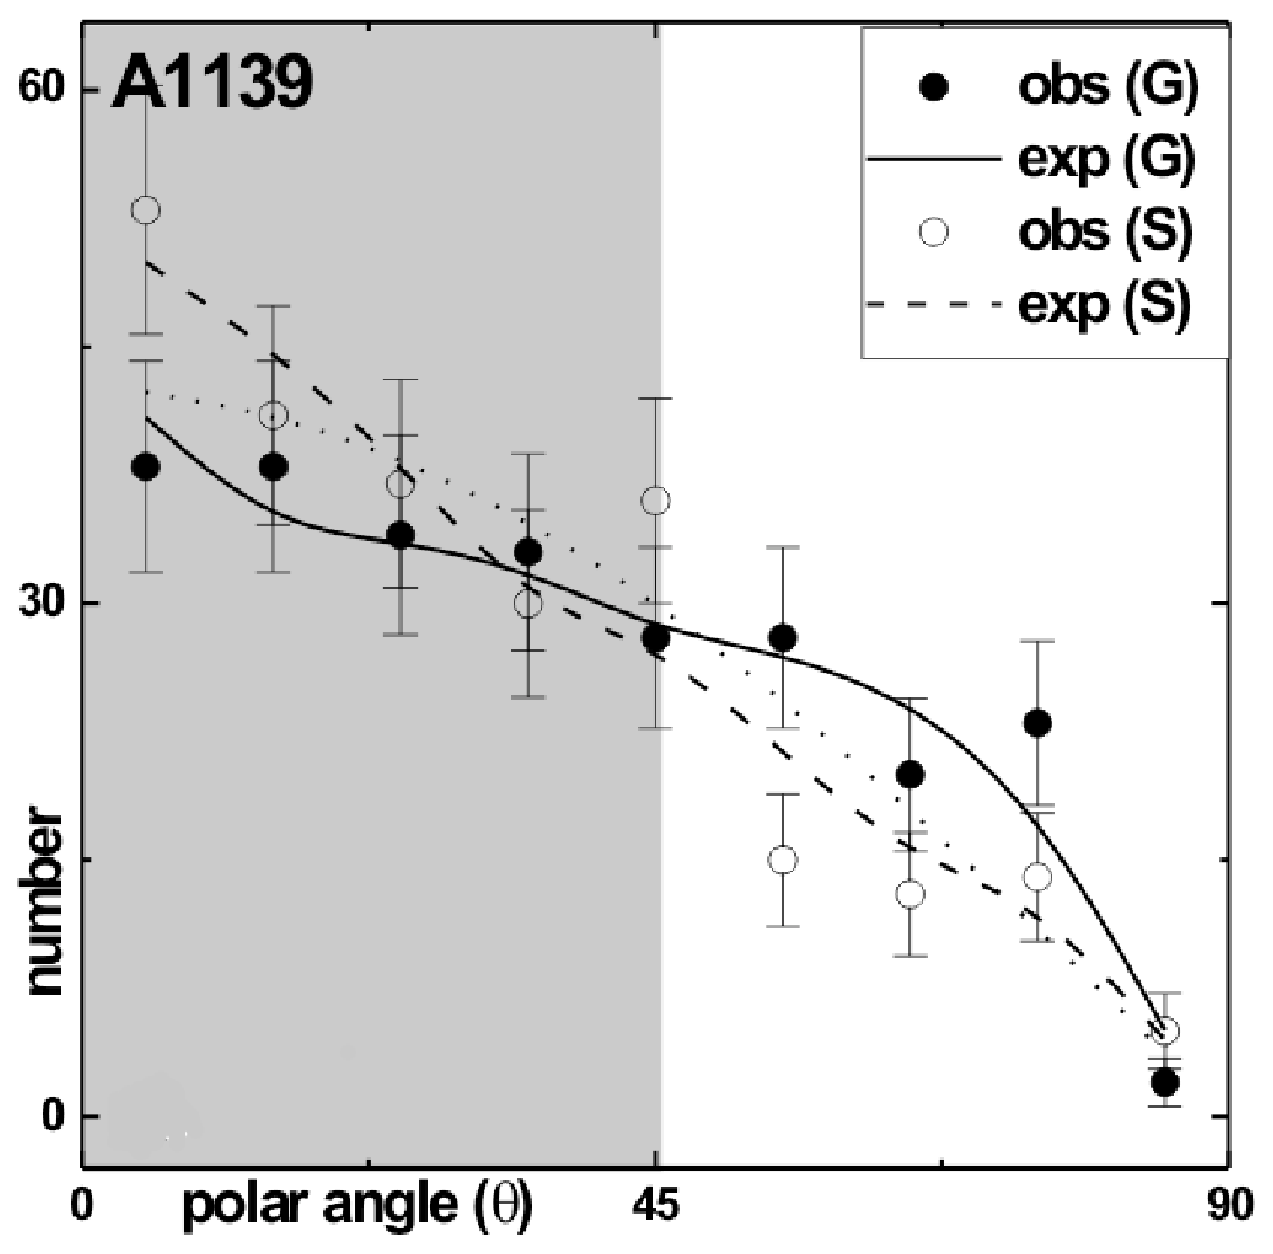
\includegraphics[height=6.9cm]{A1139_theta.eps}
      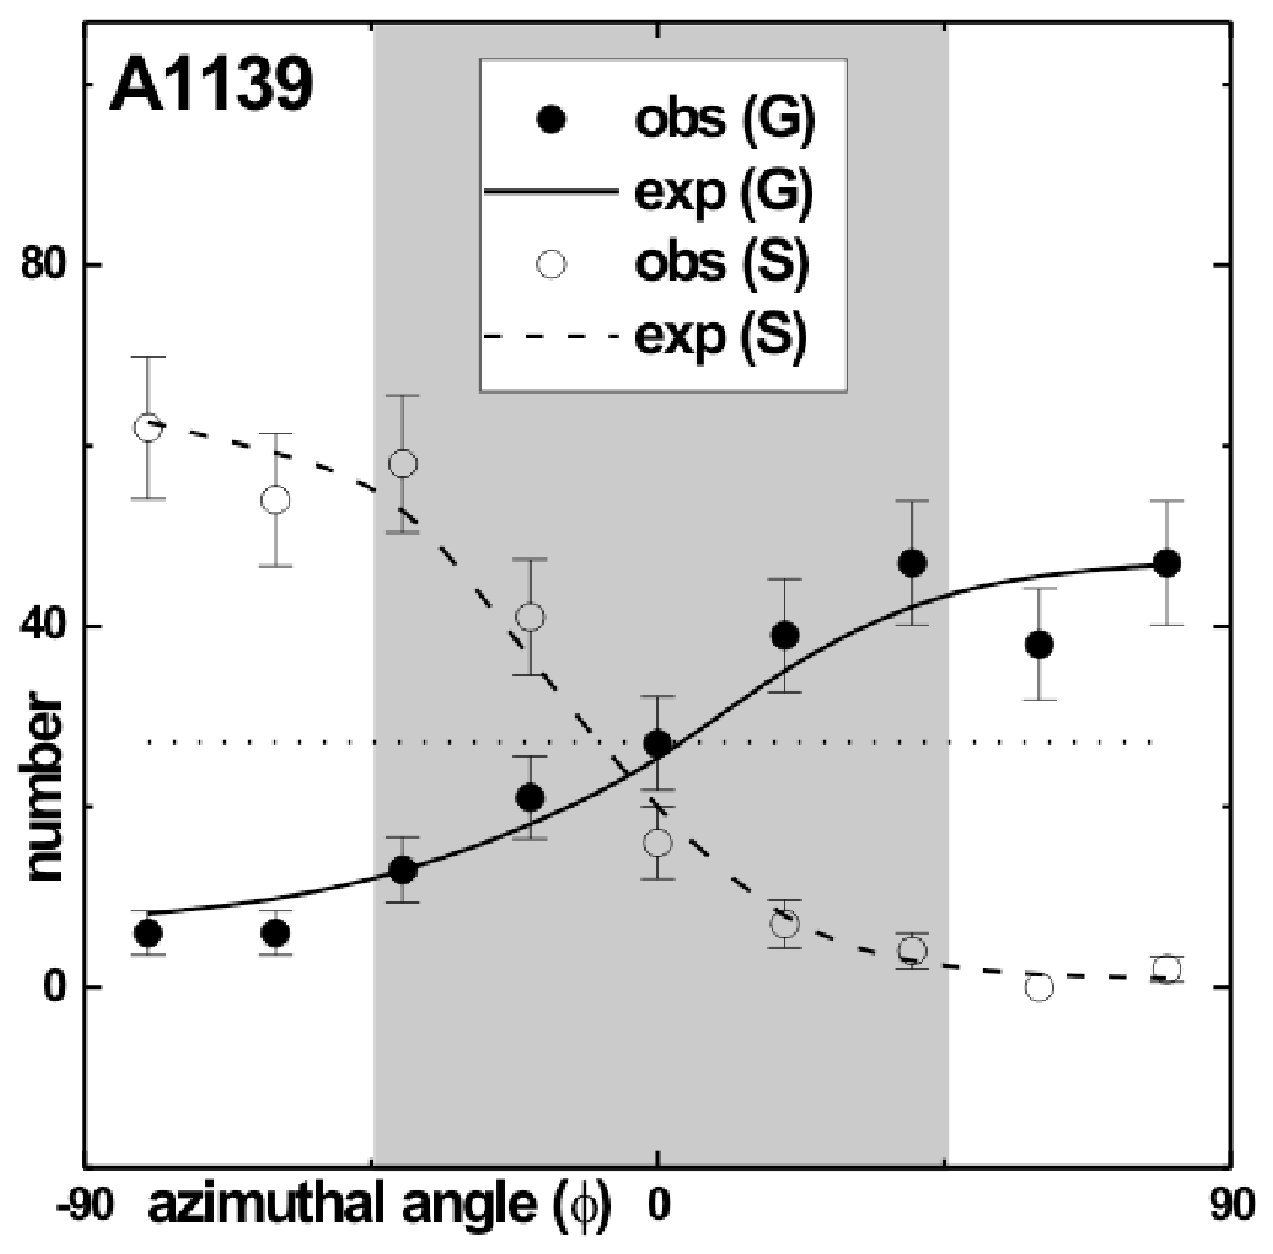
\includegraphics[height=6.9cm]{A1139_phi.eps}
            \caption[]{ The polar (left) and azimuthal angle (right) distributions of galaxies in A1139
with respect to the G (solid line) and S (dashed line) coordinate systems.
For comparison, cosine and average distributions (dotted line) are shown.
The polar angle, $\theta$ = 0$^\circ$ (90$^\circ$ ) corresponds to the galactic SV tends to lie
parallel (perpendicular) to the galactic/Supergalactic plane. The azimuthal
angle, $\phi$ = 0$^\circ$ means the direction to the galactic/Supergalactic centre. The
statistical error ($\pm\, 1\, \sigma$ ) bars are shown for the observed counts. A hump in the
grey-shaded region represents the SV of galaxies tend to lie in the reference
plane (left) and SV projections of galaxies tend to be directed towards the
centre of the reference coordinate system (right).
}
\end{figure}
\noindent All the statistical test support isotropy (see Table 5.1)
in both the $\theta$ and $\phi$ distributions suggesting a random orientation of spin vectors and spin vector projections of galaxies with respect to both galactic and Supergalactic coordinate systems. No significant humps and dips can be seen in the histogram. Our result supports the hierarchy model (Peeble 1969) in which galaxies were believed to be first formed and while they obtained angular momentum by tidal forces while they were gathering gravitationally to form clusters.\\\\
Strong isotropy in the spatial orientation of spin vectors of galaxies indicate that a single cluster in rotation rather than two overlapping clusters that either merge or depart from each other as pointed in Burgertt et al. (2004).
\subsection{Abell 2162}
Abell 2162 is one of the nearest cluster in our sample and is a member cluster in the Hercules Supercluser (Einasto et al. 2001). Neither a distinct substructure nor a significant local density peaks is found except for the cluster center. HL calculated rotational amplitude and global velocity gradient using the galaxies at inner region ($<18^\prime$, as the radial distribution was discontinuous at $\sim 18^\prime$) and found ${|v_{rot}|}/{\sigma_p}= 0.64$ and $\frac{dv}{dR}$=635, satisfying the criteria for rotating clusters.
\begin{figure}[H]
\centering
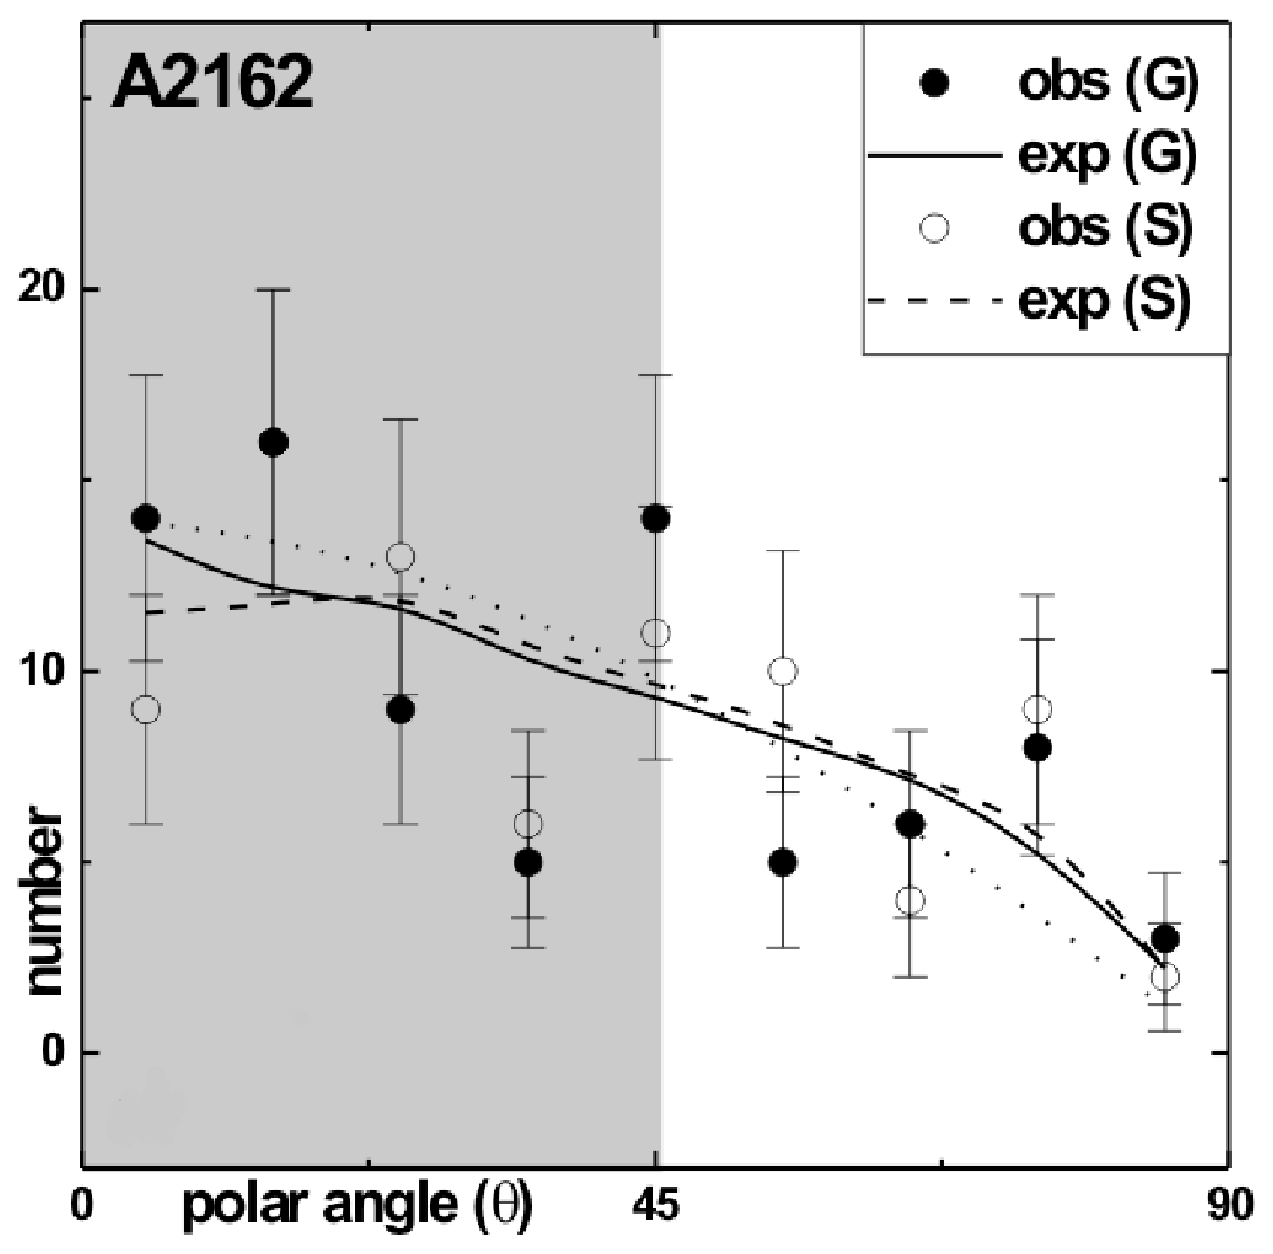
\includegraphics[height=6.9cm]{A2162_theta.eps}
   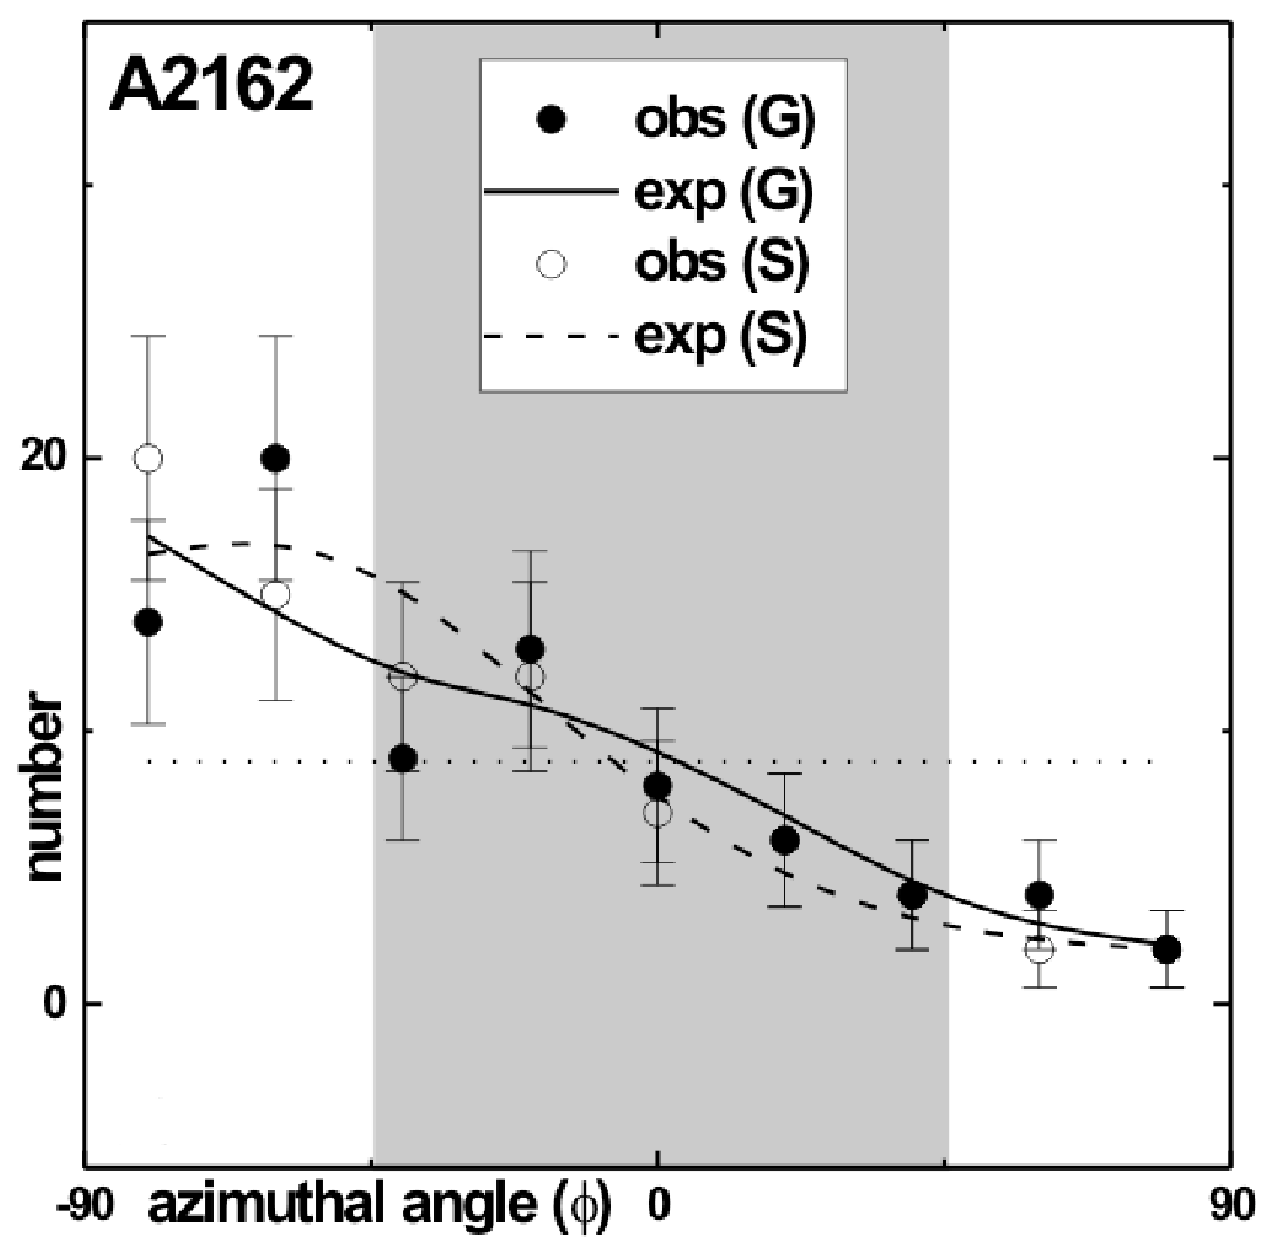
\includegraphics[height=6.9cm]{A2162_phi.eps}
      \caption{The polar (left) and azimuthal angle (right) distributions of galaxies in A2162
with respect to the G (solid line) and S (dashed line) coordinate systems.
For comparison, cosine and average distributions (dotted line) are shown.
The polar angle, $\theta$ = 0$^\circ$ (90$^\circ$ ) corresponds to the galactic SV tends to lie
parallel (perpendicular) to the galactic/Supergalactic plane. The azimuthal
angle, $\phi$ = 0$^\circ$ means the direction to the galactic/Supergalactic centre. The
statistical error ($\pm\, 1\, \sigma$ ) bars are shown for the observed counts. A hump in the
grey-shaded region represents the SV of galaxies tend to lie in the reference
plane (left) and SV projections of galaxies tend to be directed towards the
centre of the reference coordinate system (right).}
\end{figure}

\noindent A hump at $45^\circ$ and two dips at angle $35^\circ$ and $55^\circ$ can be seen in $\theta$ distribution. These humps and dips compensate each other and hence all statistical tests show isotropy (see Table 5.1). The binning effect cannot be ruled out here. Thus, no preferred alignment of spin vectors of galaxies with respect to both galactic and Supergalactic coordinate system is found. In the $\phi$ distribution, all statistical tests advocate isotropy. There is a very good agreement between the observed and expected distribution suggesting random orientation of spin vector projections of galaxies with respect to galactic and Virgo cluster center. Thus there is a good agreement between the hierarchy model and global rotation with the vanishing angular momentum is observed, suggesting the existence of Li model (Li 1998).

\subsection{Abell 2366} Jones \& Forman (1999) and Flin \& Krywult (2006) found no substructure using Einstein X-ray images and positional information of galaxies. Similarly, HL studied galaxy number density map and found no evidence of substructure, but a significant value of velocity dispersion. A weak bimodal velocity distribution with a large dispersion but weak central aggregration of galaxies was found. HL found ${|v_{rot}|}/{\sigma_p}= 0.57$ and $\frac{dv}{dR}$=788, satisfying the criteria for rotating clusters. So, they selected this as a probable rotating galaxy cluster.
\begin{figure}[H]
\centering
 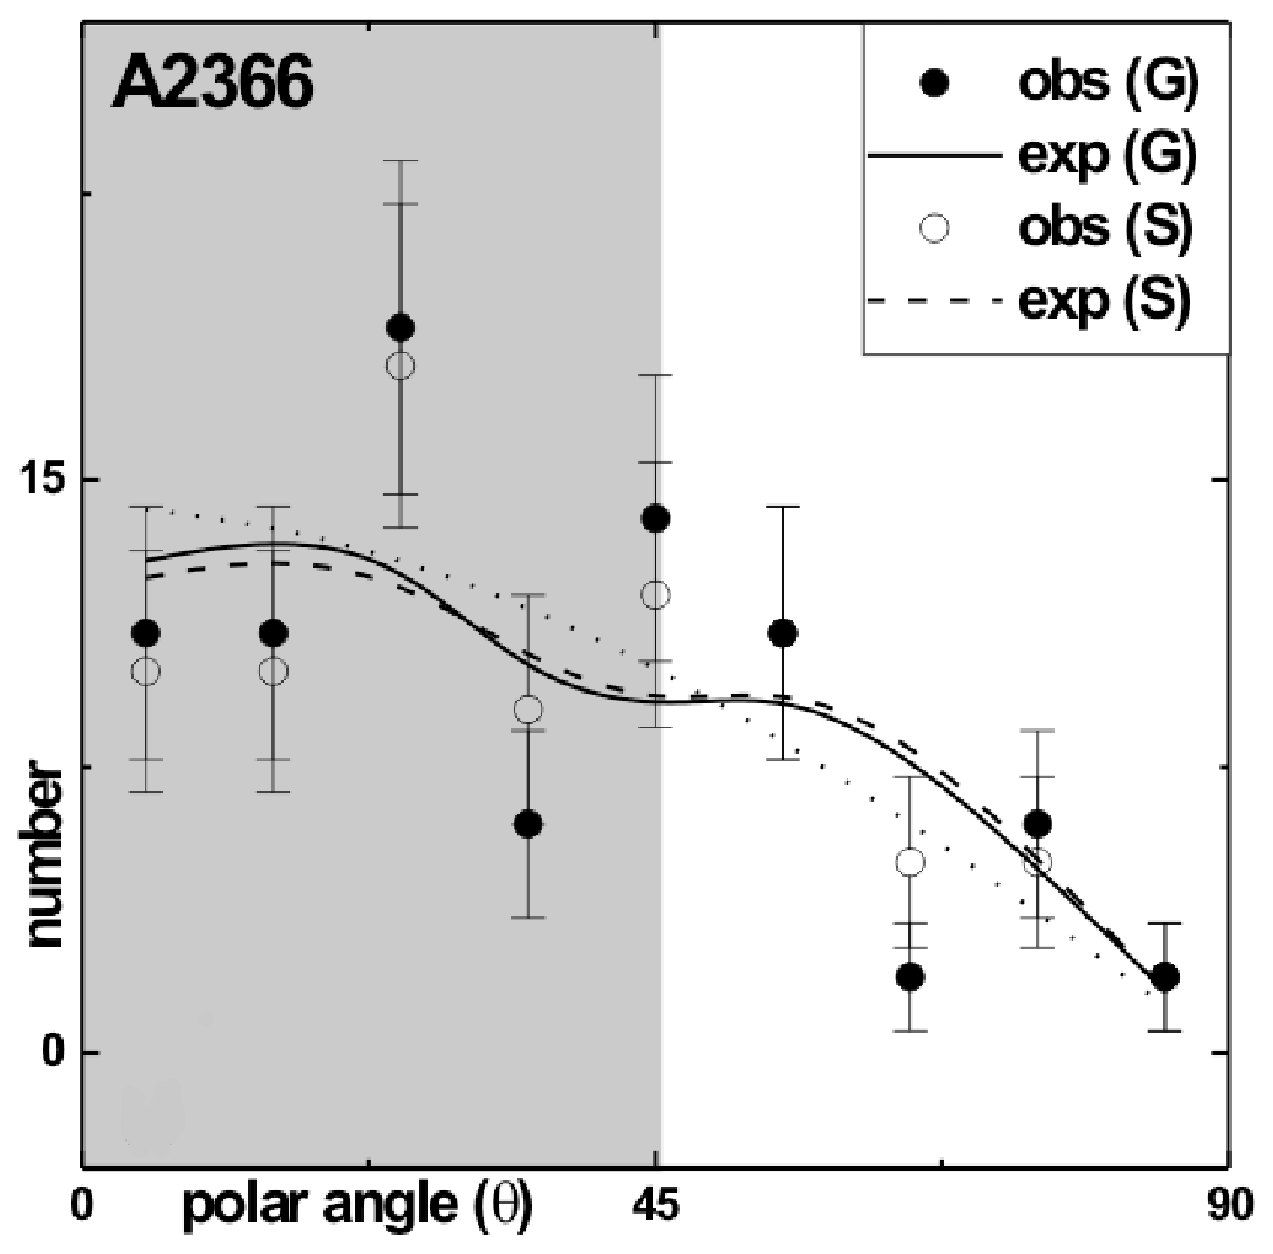
\includegraphics[height=6.9cm]{A2366_theta.eps}
   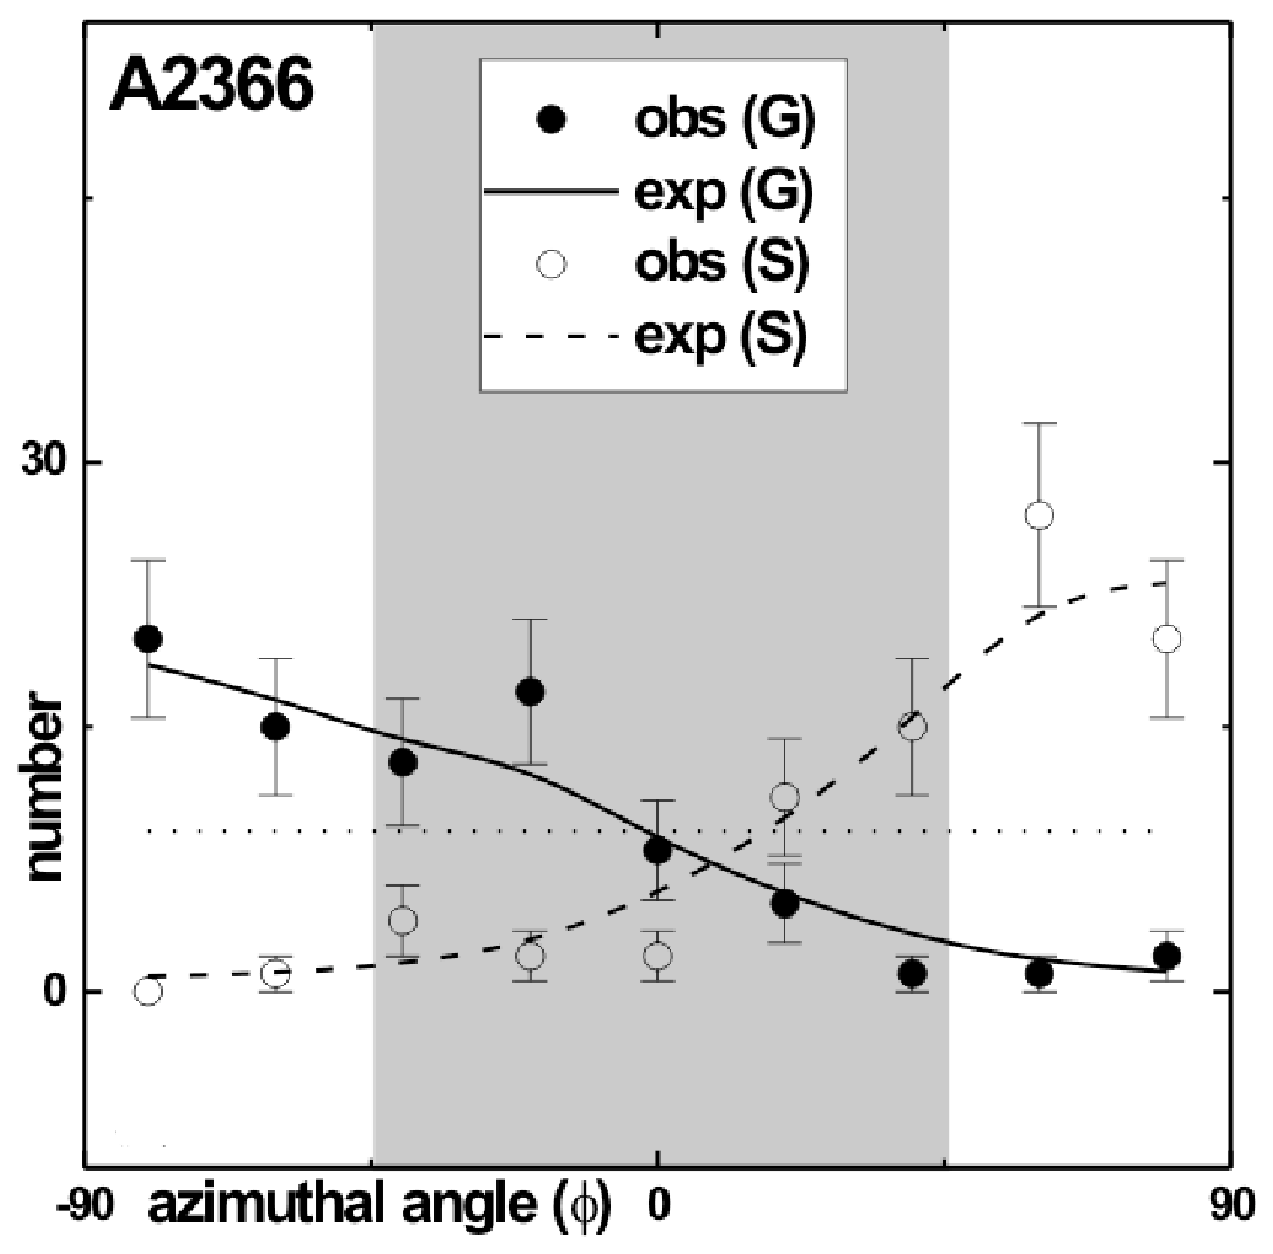
\includegraphics[height=6.9cm]{A2366_phi.eps}
     \caption{The polar (left) and azimuthal angle (right) distributions of galaxies in A2366
with respect to the G (solid line) and S (dashed line) coordinate systems.
For comparison, cosine and average distributions (dotted line) are shown.
The polar angle, $\theta$ = 0$^\circ$ (90$^\circ$ ) corresponds to the galactic SV tends to lie
parallel (perpendicular) to the galactic/Supergalactic plane. The azimuthal
angle, $\phi$ = 0$^\circ$ means the direction to the galactic/Supergalactic centre. The
statistical error ($\pm\, 1\, \sigma$ ) bars are shown for the observed counts. A hump in the
grey-shaded region represents the SV of galaxies tend to lie in the reference
plane (left) and SV projections of galaxies tend to be directed towards the
centre of the reference coordinate system (right).}
   
\end{figure}

\noindent A significant hump at $25^\circ$ followed by two dips at $35^\circ$ and $65^\circ$ can be seen in the spin vector distribution of member galaxies. These hump and dips compensate each other to show isotropy in the statistical test (see Table 5.1). A local effect can  not be ruled out here, probably due to the gravitational tidal forces due to the massive central region. In azimuthal angle distribution, a random orientation is observed in the statisitics as well as in histogram. Thus, it is found that the rotating cluster which is the dynamical equilibrium shows vanishing angular momentum as predicted by Godlowski et al. (2003) and observationaly verified by Godlwoski (2012).
\section{General Discussion}
\begin{figure}[H]
\centering
\includegraphics[height=6.9cm]{polar.eps}\\
 \includegraphics[height=6.9cm]{phi.eps}
     \caption{The orientation parameter (the First Order Fourier coefficient,  $\Delta_{11}$/$\sigma(\Delta_{11})$) plot for polar angle i.e. $\theta$ (top) and azimuthal angle i.e. $\phi$  (bottom) for three clusters with respect to the galactic and Supergalactic coordinate system. The region of isotropy is given by the shaded portion in graph.
-$1\leq\Delta_{11}$ /$\sigma(\Delta_{11})\leq +1$ for the isotropy and $\Delta_{11}/\sigma(\Delta_{11}) > \pm 1$ for anisotropy.} 
\end{figure}
\noindent From the Table 5.1 we can easily see that almost all statistical test supports isotropy of the distribution of the spin vectors of galaxy i.e. statistics supports hierarchy model. However, the first order Fourier coefficient test support anisotropy for the azimuthal angle distribution for the A1139 in galactic coordinate system. The polar angle distribution shows strong isotropy in both galactic and Supergalactic system. In case of azimuthal distribution, all the galaxies shows isotropy in Supergalactic coordinate system.\\\\
As the sign of $\Delta_{11}$ for the polar angle distribution gives the tendency of orientation  of spin vectors parallel or perpendicular to the plane of the reference coordinate system. i.e positive (negative) $\Delta_{11}$ suggests that spin vectors of galaxies tend to orient parallel (perpendicular) with respect to reference coordinate sysem. From figure 5.4 we can see angular momentum vectors of A1139 and A2366 tend to orient perpendicular to the reference plane of the galactic coordinate system but A2162 has the spin vector orientation parallel to the reference plane of the galactic coordinage system. However in case of Supergalactic coordinate system A2162 and A2366 tend to orient its angular momentum vector parallel to the plane but A1139 tend to orient it perpendicular to the plane of Supergalactic coordinate system.\\\\
The database, selection criteria, result and references of the published paper in MNRAS based on result of these three clusters (A1139, A2162, A2366) along with the result of other three clusters (A0954, A1399, A2169), which was proposed by HL as rotating clusters, is given in tabular form below:
\begin{center}
\begin{tabular}[lp=7cm]{|l|l|l|l|}
\hline\hline
Database&Selection&Results&References\\
&criteria&&\\
\hline
6 rotating&SDSS \& &- a random orientation of&Aryal,\\
clusters&2dFGRS&angular momentum vectors of&Bhattarai,\\
&database:&galaxies are found in all six&Dhakal,\\
&A954, A1139,&rotating clusters&Rajbahak \&\\
&A1399, A2162&supporting Hierarchy&Saurer\\
&A2169, and&model of galaxy&(2013)\\
&A2366&formation&\\
&&-It is found that the vanishing&\\
&&angular momentum is preferred by&\\
&&the rotating clusters which are in&\\
&&dynamical equilibrium and&\\
&&have large value of&\\
&&velocity dispersion&\\
\hline
\end{tabular}
\end{center}




%------------------------------------------------------

%\chapter{Discussion}
%
%\include{discussion}

%------------------------------------------------------
% Conclusion of present work
%------------------------------------------------------
%-------------------------------------------------------------
\chapter{Conclusion}

First we summarize the steps that we have followed in our CODE and 
then the results concerning the spatial orientation of galaxies in three
rotating clusters (A2162, A1139, A2366) that we obtained by using CODE will be discussed.
The code named GOBAD1.0 follows the following steps:
\begin{itemize}
\item It propagates number statistics in order to find appropriate bin size for given parameters. 
\item It makes input files by creating 1$0^n$ random virtual galaxies (Aryal \& Saurer 2000) for the given parameters and it gives expected polar and azimuthal angle distributions following Godlowskian method (Flin \& Godlowski 1986).
\item It calculates observed distribution by using database of galaxies that we obtained from Huyang \& Lee (2007)
\item A comparison between the observed and expected distribution can me made by using our CODE, using various statistical tests, namely $\chi^2$-test, auto-correlation test, Fourier test, K-S test and K-V test. 
\end{itemize}
We have studied spatial orientations of angular momentum vectors
of galaxies in three rotating clusters (A2162, A1139, A2366) that are in dynamical
equilibrium with a single number-density peak around the cluster
center and a spatial segregation of high- and low-velocity
galaxies. We conclude our results as follows:

\begin{itemize}
\item A random orientation is noticed for all three rotating clusters
supporting hierarchy model as predicted by Peeples (1969). The
clusters that are rotating and in the dynamical equilibrium showed
a random orientation of spin vector and spin vector projections
with respect to both galactic and Supergalactic coordinate
systems. As expected the choice of coordinate system is found to
be independent of the spatial orientation of the galaxies in the
cluster.

\item We noticed that the vanishing angular momentum is
preferred by the rotating clusters that have larger value of
velocity dispersion. The existence of substructures is probably a
signature of non-vanishing angular momenta. Thus, we found a good
correlation between hierarchy model (Peebles 1969) and the Li's
model (Li 1998) concerning the evolution of large scale
structures. 

%\item Godlowski (2011) discussed the observational aspect of
%rotations in the universe on different scales and concluded by
%advocating Li's (1998) model in which galaxies are believed to be
%formed in the rotating universe.  However the results of Aryal
%\& Saurer (2006) as well as those of Godlowski et al. (2010) are
%consistent  with the predictions of Li's model, they may be as
%well interpreted as the effect of tidal forces, according to the
%scenario of Catelan \& Theuns (1996). A  similar results are
%obtained by Aryal et al. (2007) and Godlowski et al. (2005). 
%In the hierarchical clustering model, the tidal torque scenario
%naturally arises and hence the distribution of spin angular
%momenta of galaxies become random. However a local tidal shear
%tensor can cause a local alignment of rotational axes (Dubinski
%1992, Lee \& Pen 2000, Lee 2004, Trujillo et al. 2006). 

\end{itemize}
\section{Future Works}

Following works are recommended for the future:
\begin{itemize}
 \item In the future we intend to study preferred alignments in the rotating
cluster candidates that are not in the dynamical equilibrium.
\item In future we intend to define a physical reference plane to study the distribution of the spin vector orinetation.

\end{itemize}


%------------------------------------------------------
% Future Prospectus
%------------------------------------------------------
%\input{Future}


%-------------------------------------------------------

\thispagestyle{plain} \mark{RREFERENCE}
\addcontentsline{toc}{chapter}{References} \noindent
{\bf REFERENCES}\\
\\
Abell G. O., Corwin H. G., Olowin R. P., ApJS, \textbf{70}, 1 (1989)\\\\
Aryal B., Bachchan R. K., Saurer W., BASI, \textbf{38}, 165 (2010)\\\\
Aryal B., Bhattarai H., Dhakal S., Rajbahak C., Saurer W., MNRAS, \textbf{434}, 3, 1939 (2013)\\\\
Aryal B., Kafle P., Saurer W., MNRAS, \textbf{389}, 741 (2008)\\\\
Aryal B., Kandel S. M., Saurer W., A \& A, \textbf{458}, 2, 357 (2006)\\\\
Aryal B., Neupane D., Saurer W., Astrophysics and Space Science, \textbf{314}, 177 (2008)\\\\
Aryal B., Paudel R. R., Saurer W., Ap \& SS, \textbf{337}, 313 (2012)\\\\
Aryal B., Paudel S., Saurer W., A \& A, \textbf{479}, 2, 397 (2008)\\\\
Aryal B., Paudel S., Saurer W., MNRAS, \textbf{379}, 1011 (2007)\\\\
Aryal B., Research in Astronomy and Astrophysics, \textbf{11}, 293 (2011)\\\\
Aryal B., Saurer W., MNRAS, \textbf{366}, 438 (2006)\\\\
Aryal B., Saurer W., MNRAS, \textbf{360}, 125 (2005)\\\\
Aryal B., Saurer W., A \& A, \textbf{425}, 871 (2004)\\\\
Aryal B., Saurer W., A \& A, \textbf{364}, L97 (2000)\\\\
Aryal B., Yadav S. N., Saurer W., BASI, \textbf{40}, 65 (2012)\\\\
Baier F. W., Babelsberg P., Ziener R., Tautenburg, AN, \textbf{ 310}, 1, 7 (1989)\\\\
Baier F. W., Godlowski W., MacGillivray H.T., A \& A, \textbf{403}, 847 (2003)\\\\
Bautz L. P., Morgan W. W., Ap J, \textbf{162}, L149 (1970)\\\\
Biviano A., Durret F., Gerbal D., Le Fevre O., Lobo C., Mazure A., Slezak E., A \& A, \textbf{311}, 95 (1996)\\\\
Bohringer H., Schuecker P., Guzzo L., Collins C.A., Voges W., Cruddace R.G., Ortiz-Gil, A. et al., A \& A, \textbf{425}, 367 (2004)\\\\
Bsyudki D. J., Burns J. O., Degg H. J., Laubscher B. E., Hill J. M., Newberry M. V., Elston R. J., AJ, \textbf{ 101}, 1983 (1991)\\\\
Burgett W. S., Vick M. M., Davis D.S., Colless M., de Propris R., Baldry I., Baugh C. et al., MNRAS, \textbf{352}, 605 (2004)\\\\
Catelan P., Theuns T., MNRAS, \textbf{282}, 2, 455 (1996)\\\\
Carter D., Bridges T. J., Hau G. K. T., MNRAS, \textbf{307},  1, 131 (2008)\\\\
Ciufolini I.,  Wheeler J. A., Gravitation and Inertia, Princeton University Press, Princeton (1995)\\\\
Colless M., Dalton G., Maddox S., Sutherland W., Norberg P., Cole S., Bland-Hawthorn J., et al., MNRAS, \textbf{328}, 1039 (2001)\\\\
Cox C. V., Bregman J. N., Schombert J. M., AJS, \textbf{99}, 405 (1995)\\\\
Dale D. A, Giovanelli R., Haynes M. P., Campusano L. E., AJ, \textbf{114}, 455 (1997)\\\\
de Ruiter H. R., Parma P., Capetti A., Fanti R., Morganti R., Santantonio L., A \& A, \textbf{ 439},  2, 487(2008)\\\\
Diaferio A., Geller M. J., Ap J, \textbf{481}, 633 (1997)\\\\
Diaferio A., MNRAS, \textbf{309}, 610 (1999)\\\\
Dubinski J., Ap J, \textbf{401}, 441 (1999)\\\\
Dupke R. A., Bregman J. N., Ap J, \textbf{547}, 705 (2001a)\\\\
Dupke R. A., Bregman J. N., Ap J, \textbf{562}, 266 (2001b)\\\\
Dong R., Rasmussen J. Mulchaey J. S., AJ, \textbf{712},  2, 883 (2010).\\\\
Donzelli, C. J., Muriel, H., Madrid, J. P., AJS, \textbf{195},  2, 17 (2011)\\\\
Doroshkevich A.G., Ap J, \textbf{14}, L11 (1973)\\\\
Ebeling H., Edge A. C., Allen S. W., Crawford C. S., Fabian A. C., Huchra J. P., MNRAS, \textbf{318},  2, 333 (2008)\\\\
Efstathiou G., Moody S., Baugh C., Bland-Hawthorn J., Bridges T.J., Cannon R.D., Cole S.M.et al., MNRAS, \textbf{330}, 29 (2002)\\\\
Einasto M., Einasto J., Tago E., Mueller V., Andernach, H., AJ, \textbf{122}, 2222 (2001)\\\\
Fanti C., Fanati R., Feretti L., Ficarra A., Gioia I. M., Giovannini G., Gregorini L., Mantovani F. et al.,A \& A, \textbf{105},  1, 200 (1982)\\\\
Flin P., Biernacka M., Godłowski W., Panko E., Piwowarska P., Baltic Astronomy, \textbf{20}, 251 (2011)\\\\
Flin P., MNRAS, \textbf{325}, 49 (2001)\\\\
Flin P., Krywult J., A \& A, \textbf{450}, 9 (2006)\\\\
Flin P., Godlowski W., MNRAS, \textbf{222}, 525 (1986)\\\\
Fritsch C., Buchert T.,A \& A, \textbf{344}, 749 (1999)\\\\
Gal R. R., de Carvalho R. R., Brunner R., Odewahn S.C, Djorgovski S.G, AJ, \textbf{120},  2, 540 (2000)\\\\
Gamow, G., Nature, \textbf{158}, 549 (1946)\\\\
Giacintucci S., Venturi T., Murgia M., Dallacasa D., Athreya R., Bardelli S., Mazzotta P., Saikia D.J., A \& A, \textbf{ 476},  1, 99 (2007)\\\\
Godlowski W., Ap J, \textbf{747}, 1, 7 (2012)\\\\
Godlowski W., IJMDP, \textbf{20}, 9, 1643 (2011)\\\\
Godlowski W., Ostrowski M., MNRAS, \textbf{303}, 50 (1999)\\\\
Godlowski, W., Piwowarska, P., Panko, E., Flin, P., Ap J, \textbf{723}, 2, 985 (2010)\\\\
Godlowski, W., Szydlowski, M., Flin, P., Biernacka, M., General Relativity and Gravitation, \textbf{35}, 907 (2003)\\\\
Godlowski, W., Szydlowski, M., Flin, P., General Relativity and Gravitation, \textbf{37}, 615 (2005)\\\\
Godlowski W., MNRAS, \textbf{271}, 19 (1994)\\\\
Godlowski W., MNRAS, \textbf{265}, 874 (1993)\\\\
Gregory S. A., Thompson L. A., Ap J, \textbf{213}, 345 (1977)\\\\
Gregory S. A., Tifft W. G., Ap J, \textbf{205}, 716 (1976)\\\\
Harrison C. D., Colless M., Kuntschner H., Couch W. J., de Propris R., Pracy M. B., MNRAS, \textbf{409},  4, 1455 (2010)\\\\
Hawley D. L., Peebles P. J. E., AJ, \textbf{80}, 477 (1975)\\\\
Haynes M., Giovanelli R., AJ, \textbf{89}, 6, 758 (1984)\\\\
Henriksen M., AJ, \textbf{103}, 1051 (1992)\\\\
Hilton M., Collins C., de Propris R., Baldry I. K., Baugh C. M., Hawthron J. B., Bridges T. et al., MNRAS, \textbf{363},  2, 661 (2013)\\\\
Holden B. P., Franx M., Illingworth G. D., Postman M., van der Wal A., Kelson D. D., Blakeslee J. P. et al.,  AJ, \textbf{693},  1, 617 (2009)\\\\
Holmberg, E., Medd. Lund. Astron. Obs., Ser. \textbf{VI}, 117 (1946)\\\\
Hubble E., Ap J, \textbf{64}, 321H (1926)\\\\
Hu F. X., Wu G. X., Su H. J., Liu Y. Z., A \& A, \textbf{302}, 45 (1995)\\\\
Hu F. X., Wu G. X., Song G. X., Yuan Q. R., Okamura S., Ap \& SS, \textbf{302}, 43 (2006)\\\\
Hu F. X., Yuan Q. R., Su H. J., Wu G. X., Liu Y.Z., Ap J, \textbf{495}, 179 (1998)\\\\
Hwang, H.S., Lee, M.G., Ap J, \textbf{662}, 236 (2007)\\\\
Jaaniste J., Saar E., in Longair M. S., Einasto J., eds., The Large Scale Structure of the
Universe, Proc. IAU Symp. No. \textbf{79}, Reidel Dordrecht, 448 (1978)\\\\
Jones C., Forman W., Ap J, \textbf{511}, 65 (1999)\\\\
Kalinkov M., Valchanov T., Valtchanov I., Kuneva I., Dissanska M., MNRAS, \textbf{359}, 1491 (2005)\\\\
Kanji, G. K., 100 Statistical Tests. Sage, Thousand Oaks (1995)\\\\
Kashikawa N., Okamura S., PASJ, \textbf{44}, 493 (1992)\\\\
Kitzbichler M. G. Sauer W., Astronomische Nacrichten, Supplementary  3, \textbf{324}, 166 (2003)\\\\
Krywult J., MacGillivary H. T., Flin P., A \& A, \textbf{351}, 883 (1999)\\\\
Kuiper, N. A., in Proc. Kononklijke Ned. Akad.Wetenschappen, \textbf{A 63}, 38 (1962)\\\\
Lambas D. G., Groth E. J., Peebles P. J. E., AJ, \textbf{95},996 (1988)\\\\
Lauer T. R, Postman M., AJ,\textbf{ 425},  2, 418 (1994)\\\\
Lahav O., Bridle S.L., Percival W.J., Peacock J.A., Efstathiou G., Baugh C.M., Bland-Hawthorn J. et al., MNRAS, \textbf{333}, 961 (2002)\\\\
Ledlow M. J., Voges W., Owen F.N., Burns J.O., AJ, \textbf{126}, 2740 (2003)\\\\
Lee J., Pen U., Ap J, \textbf{532}, 1, L5 (2000)\\\\
Lee J., Ap J, \textbf{614}, 1, L1 (2004)\\\\
Li L. X., General Relativity and Gravitation, \textbf{30}, 497 (1998)\\\\
Liuzzo E., Giovannini G., Giroletti M., Taylor G. B., A \& A, \textbf{ 516}, A1, 15 (2008)\\\\
Mahdavi A., Geller M. J., AJ, \textbf{ 554},  2, 129 (2001)\\\\
Materne J., Hopp U., A \& A, \textbf{124}, L13 (1983)\\\\
McDonald M., Veilleux S., Mushotzky R., AJ, \textbf{ 731},  1, 12 (2011)\\\\
Miller N. A., AJS, \textbf{ 134},  2, 355 (2001)\\\\
Oegerle W.R., Hill J.M., AJ, \textbf{104}, 2078 (1992)\\\\
Pajowska P., Godlowski W., Panko E., Flin P., Journal of Physical Studies, \textbf{16}, 4901 (2012)\\\\
Peebles P. J. E., Ap J, \textbf{155}, 393 (1969)\\\\
Percival W.J., Baugh C.M., Bland-Hawthorn J., Bridges T.J., Cannon R.D., Cole S., Colless M.M. et al., MNRAS, \textbf{327}, 1297 (2001)\\\\
Plionis M., AJS, \textbf{ 95},  2, 401 (1994)\\\\
Plionis M., Barrow J. D., Frenk C. S., MNRAS, \textbf{ 249}, 662 (1991)\\\\
Poggianti B. M., von der Linden A. A., de Lucia G., Desai V., Simard L., Halliday C., Bower R. et al., AJ, \textbf{ 642},  1, 188 (2004)\\\\
Popesso P., Biviano A., Bohringer H., Romaniello M., A \& A, \textbf{ 461},  2, 397 (2007)\\\\ 
Postman M., Huchra J. P., Geller M. J., AJ, \textbf{ 384}, 404 (1992)\\\\
Press, W. H., Teukolsky, S.A., Vetterlin, W.T., Flannery, B.P. in Numerical Recipes in C, 2nd ed. Cambridge University Press, Cambridge (1992)\\\\
Regos E., Geller M. J., AJ, \textbf{98}, 3, 755 (1989)\\\\
Rines K., Geller M. J., Kurtz M. J., Diaferio A, AJ, \textbf{126}, 2152 (2003)\\\\
Rohinson M. R., Sharpe J., Oliver S. J., Keeble O., Canavezes A., Saunders W., Taylor A. N. et al., MNRAS, \textbf{ 314},  2, 375 (2008)\\\\
Sandage A., Perelmuter J. M., AJ, \textbf{ 370}, 455 (1991)\\\\
Schombert J. M., AJ, \textbf{ 328}, 475 (1988) \\\\
Seward F. D., Charles P. A., Exploring the X-ray Universe, 2nd ed. Cambridge University Press, Cambridge (2010)\\\\
Shandarin S. F., Astr. Zh \textbf{51}, 667 (in Russian), Soviet Astron \textbf{18}, 392 (in English) (1974)\\\\
Stephens, M. A., in J. R. Stat. Soc. B \textbf{32}, 115 (1970)\\\\
Struble M. F., Rood H. J., AJS,\textbf{ 77}, 363 (1991)\\\\
Sun M., Voit G. M., Gonahue M., Jones C., Forman W., Vikhlinin A., AJ, \textbf{ 693},  2, 1142 (2009)\\\\
Tammann G. A., Sandage A., ApJ, \textbf{207}, L1 (1976)\\\\
Tovmassian H., astro-ph/021211 (2002)\\\\
Torlina L., De Propris R, West M. J., AJ ,\textbf{660}, L97, (2007)
Trujillo I., Carretero C., Patiri S. G., ApJ, \textbf{640}, 2, L111 (2006)\\\\
van Haarlem M. P., Cayon L., Cruz C. G., Martinez-Gonzalez E., Rebolo R., MNRAS, \textbf{264}, 71 (1993)\\\\
Verde L., Heavens A.F., Percival W.J., Matarrese S., Baugh C.M., Bland-Hawthorn J., Bridges T.J. et al., MNRAS, \textbf{335}, 432 (2002)\\\\
Vogt N. P., Haynes P. M., Herer T., Giovanelli R., AJ, \textbf{ 127},  6, 3273 (2004)\\\\
von Weizs ̈cker, C. F., Ap J, \textbf{114}, 165 (1951)\\\\
Weinberg S., Gravitation and Cosmology, John Wiley \& Sons (1972)
West M. J., AJ, \textbf{ 347}, 610 (1989)\\\\
White R. A., AJ, \textbf{ 226}, 591 (1978)\\\\
Willick J. A., AJ, \textbf{ 516},  1, 47 (1998)\\\\
Wise M. W., O'Connell R. W., Bregman J. N., Roberts M., AJ, \textbf{ 405},   1, 94 (1992)\\\\
Wojtak R., Lokas E. L., MNRAS, \textbf{ 408},  4, 2442 (2010)\\\\
Wu X. P., Han J., MNRAS, \textbf{ 272},  4, 705 (1994)\\\\
Wu G. X., Hu F. X., Su H. J., Liu, Y. Z., A \& A, \textbf{323}, 317 (1997)\\\\
Yanny B., Rockosi C., Jo N. H., Knapp G. R., Jennifer K. A.,Alcorn B., Allam S., AJ, \textbf{137}, 4377 (2009)\\\\
Yuan Q. R., Hu F. X., Su H. J., Huang K. L., A J, \textbf{114}, 1308 (1997)\\\\
%--------------------------------------------------------------------------------------------
%A\&A----Astronomy Astrophysics
%AJ-----Astronomical Journal
%AJS-----------------The Astrophysical Journal Supplement
%AN-----------------------Astronomische Nachrichten
%PASJ: Publication Astronomy Society Japan
%BASI----	Bulletin of the Astronomical Society of India
%------------------------------------------------------------------------------------------------------
%A1139
\textbf{\Large{Web:}}\\\\
1. http://www2.aao.gov.au/$\sim$TDFgg/\\
2. http://www.fnal.gov/pub/today/archive/archive\_2005/today05-05-04.html\\\\\\
\textbf{\Large{Abbreviation:}}\\\\
A \& A -------------------Astronomy Astrophysics\\\\
AJ-----------------------Astronomical Journal\\\\
AJS----------------------The Astrophysical Journal Supplement\\\\
AN-----------------------Astronomische Nachrichten\\\\
PASJ-------------------- Publication Astronomy Society Japan\\\\
BASI----	-----------------Bulletin of the Astronomical Society of India\\\\
Ap J---------------------Astrophysical Journal\\\\
MNRAS--------------------Monthly Notice of Royal Astronomical Society\\\\














%-----------------------------------------------------------------------
%-2366








%------------------------------------------------------
% Appendix
%------------------------------------------------------
\begin{appendix}

%-----------------------------------------------------
%Godlwoski transformation equation
%------------------------------------------------------------------------
\chapter{Godlowskian Transformation}\label{God}
%------------------------------------------------------------------------
The derivation of the basic formula is given considering the
distribution of galaxies within the LSC \& its PA in galactic
system. Let us consider a equatorial coordinate system, hereafter
referred to as the E system. An observer is situated at the origin
of the E system which is at the center of our galaxy. The X-Y
plane represents the plane of the E system (i.e, the plane of the
Milky way) and the coordinates $\alpha$ and $\delta$ represent the
equatorial longitude and latitude, respectively. The X-axis,
called EX is directed towards the center of the equatorial plane
($\alpha$ = 0, $\delta$ = 0). The Y and Z-axis known as EY and EZ
are directed towards the point $\alpha$ = $\pi$/2, $\delta$ = 0
and north equatorial pole ($\alpha$ = $\pi$/2, $\delta$ =
$\pi$/2), respectively.
\\
\\
Let us consider another coordinate system. The origin of the this
system is at the galaxy center. In this system, U and V-axes are
perpendicular to each other and tangent to the celestial sphere.
The U-axis is parallel to the equatorial latitude. The W-axis is
perpendicular to both U and V-axes and is the extension of the
connecting line between the centers of the cluster to the center
of galaxy. This axis points out of the sphere. These can be seen
in Fig. A1. Fig. A2 shows the detailed view of the galaxy
showing the vectors described above. The angle $q$ is an angle
between the U-axis and the projection of galaxy major axis $a$ on
the celestial sphere. The minor axis is denoted by $b$. The angle
$q$ is related to the equatorial position angle $p$, measured in
the equatorial coordinate system is given by the expression: $q$ =
$p$$-$$\pi$/2 and is measured from $-$$\pi$/2 to $+$$\pi$/2.
\\\\
\begin{figure} \vspace{0.0cm}
      \centering
      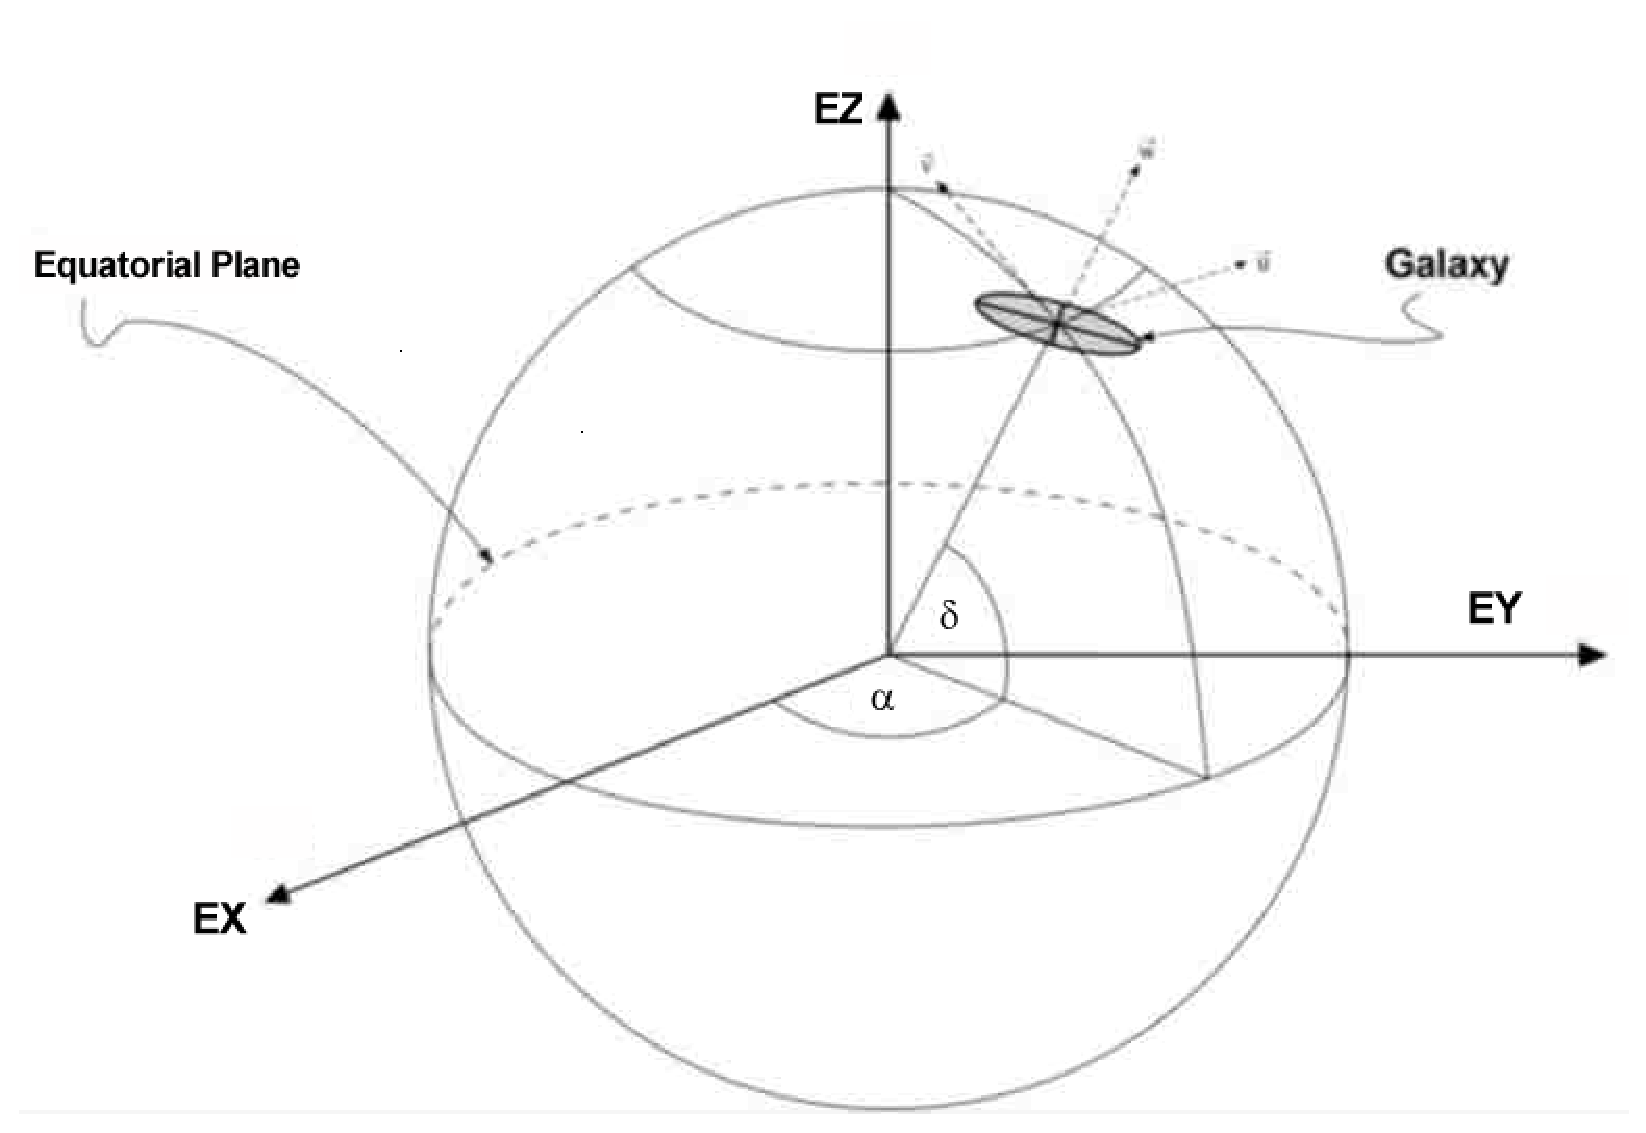
\includegraphics[height=10cm]{Godlowski1}
      \caption[]{The coordinate system used for the derivation of the polar and
azimuthal angle of the galaxy rotation axes. Here $\alpha$ and
$\delta$ represent right ascension and declination of the galaxy.
[source: Aryal 2002] }
\end{figure}
\begin{figure} \vspace{0.0cm}
      \centering
      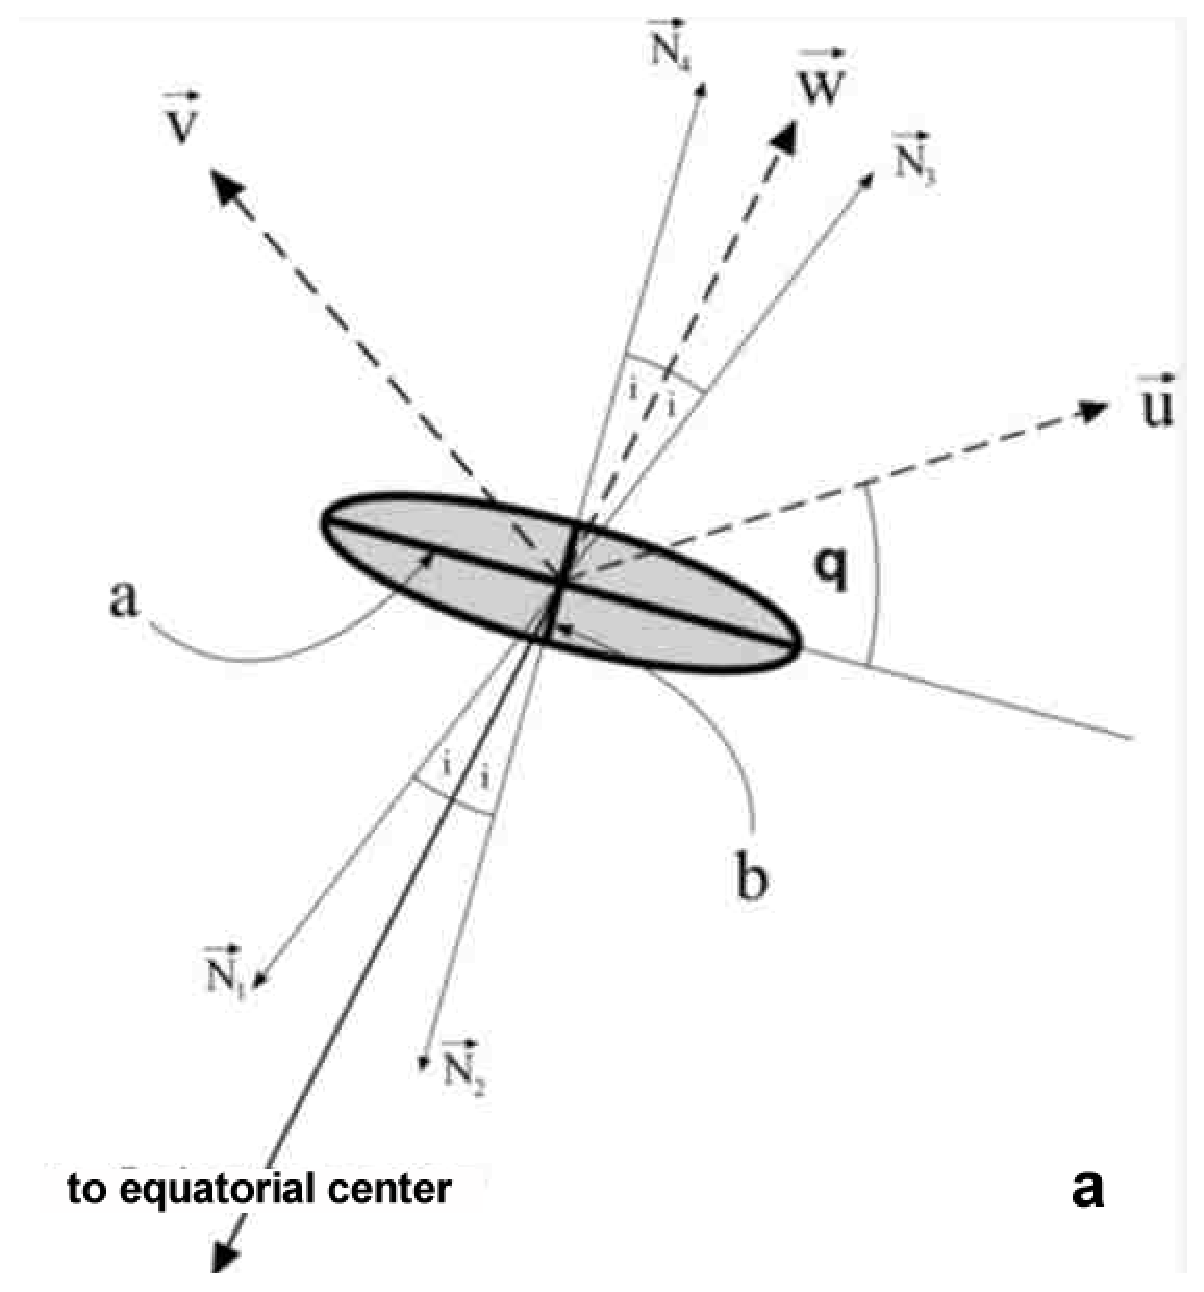
\includegraphics[height=7.7cm]{Godlowski2}
      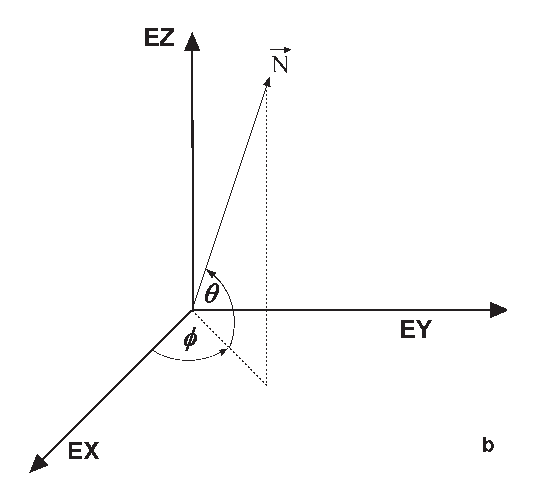
\includegraphics[height=7.7cm]{Godlowski3}
      \caption[]{(a) Detailed view on a galaxy: $a$ and $b$ are the major
      and the minor axes, $q$ = $p$ -- $\pi$/2, N$_1$ and N$_2$ corresponds to the
      two possible rotation axes. (b) Definition of the two angles $\theta$ and $\phi$
      which contain the orientation of the spin vector $N$ with respect
      to the equatorial coordinate system. [source: Aryal 2002]}
\end{figure}
\\
\\
Let us extend the normal to the galaxy plane passing through the
origin of equatorial system. For an inclination angle, $i$, there
will be two possible normals N$_1$ and N$_2$, and hence two
possible positions of the galaxy rotation axis. The angular
momentum vector is situated along one of these two normals.  Let
us consider N$_1$ and N$_2$ as the galaxy angular momentum
vectors. It is seen from the Fig. A2.a that there are other two
spin vectors N$_3$ and N$_4$ oriented just opposite to N$_1$ and
N$_2$. N$_1$ and N$_3$ can be identified as one rotation axis
whereas N$_2$ and N$_4$ as second rotation axis. So the ambiguity
of four solutions for the spin vectors can be reduced to an
ambiguity of two solutions. Therefore just N$_1$ and N$_2$ are
used for the statistical investigation.
\\
\\
The vectors N$_1$ and N$_2$ in the E system are
\begin{equation}\label{N}
\begin{array}{l}
$N$_1$$ = - W\cos i + \sin i (V \cos q + U \sin q)\\
\\
$N$_2$$ = - W\cos i - \sin i (V \cos q + U \sin q)\\
\end{array}
\end{equation}
%----------------------------------------------------------------------------------
Where cos$i$ is given by Holmberg's equation with the flatness
factor q* and is
%----------------------------------------------------------------------------------
\begin{equation}
\begin{array}{l}
\cos^2 i = \frac{[(b/a)^2 - (q*)^2]}{1 - (q*)^2}
\end{array}
\end{equation}
%----------------------------------------------------------------------------------
and ($V\cos q\, +\, U\sin q$) is the projection of the normals to the U-V
plane. Now we apply the method of coordinate translation here. The
galaxy related reference frame is translated to the center of the
E system. This translation allows us to express the coordinates U,
V and W in the E system. In the E system, these coordinates are
the functions of right ascension ($\alpha$) and declination
($\delta$) only and they can be written as follows:
%-------------------------------------------------------------------------------
\begin{equation}\label{UVW}
\begin{array}{l}
U = (-\sin \alpha, \ cos \alpha, 0)\\
\\
V = (-\sin \delta\cos \alpha, \cos \delta\sin \alpha, \cos \delta)\\
\\
W = (\cos \delta\cos \alpha, \cos \delta\sin \alpha, \sin \delta)\\
\\
\end{array}
\end{equation}
%--------------------------------------------------------------------------------
here, $-$sin$\alpha$, cos$\alpha$ and 0 are the functions of the
vector U along X, Y and Z axes, respectively. Similarly,
$-$sin$\delta$cos$\alpha$, $-$sin$\delta$sin$\alpha$, cos$\delta$
and cos$\delta$cos$\alpha$, cos$\delta$sin$\alpha$, sin$\delta$
are the functions of the vectors V and W along X, Y and Z
directions, respectively.
\\
\\
Substituting the values of U, V and W from equation \eqref{UVW} in
\eqref{N} we get,
%------------------------------------------------------------------------------------
\begin{equation}\label{N_12}
\begin{array}{l}
$N$_{ix}$$ = - \cos i\cos \delta\cos \alpha + \sin i(\mp \cos q \sin \delta \cos \alpha \mp \sin q\sin \alpha); \\
\\
$N$_{iy}$$ = - \cos i\cos \delta\sin \alpha + \sin i(\mp \cos q \sin \delta \sin \alpha \pm \sin q\cos \alpha); \\
\\
$N$_{iz}$$ = - \cos i\cos \delta \pm \sin i\cos q\cos \delta ; \\
\end{array}
\end{equation}
%-------------------------------------------------------------------------------------

where the upper and lower signs are for $i$ =1 and 2,
respectively.
\\
\\
Now we introduce two angles: polar ($\theta$) and azimuthal angle
($\phi$) of galaxy rotation axis. The polar angle ($\theta$), is
the angle between the N$_i$ vector and the galactic plane. The
angle between the X-axis and the projection of the N$_i$ vector on
the galactic plane is termed as the azimuthal angle ($\phi$). It
should be noted that the reversal of the vectors N$_1$ and N$_2$
transforms the $\theta$ and $\phi$ values into $-$$\theta$ and
$\phi$ + $\pi$., respectively.
\\
\\
From Fig. A2 b, we can write,
\begin{equation}\label{theta_phi}
\begin{array}{l}
$N$_{ix}$$ =  \cos \theta\cos \phi; \\
\\
$N$_{iy}$$ =  \cos \theta\sin \phi;  \\
\\
$N$_{iz}$$ =  \sin \theta. \\
\end{array}
\end{equation}\\
%--------------------------------------------------------------------------------
Comparing the equations \eqref{theta_phi} and \eqref{N_12} gives,
%-------------------------------------------------------------------------------
\begin{equation}\label{theta_phi_delat1}
\begin{array}{l}
\sin \theta = -\cos i\sin \delta \pm \sin i\cos q\cos \delta;\\
\\
\sin \phi = \frac{- \cos i\cos \delta\sin \alpha + \sin i(\mp \cos q \sin \delta\sin \alpha \pm \sin q\cos \alpha)}{\cos \theta};\\
\\
\cos \phi = \frac{- \cos i\cos b\cos \alpha + \sin i(\mp \cos q \sin \delta\cos \alpha \mp \sin q\sin \alpha)}{\cos \theta}.\\
\end{array}
\end{equation}\\
%---------------------------------------------------------------------------------------
Substituting q = $p$ $-$ $\pi$/2 in equation \eqref{theta_phi_delat1},
%--------------------------------------------------------------------------------------
\begin{equation}\label{theta_phi_delta2}
\begin{array}{l}
\sin \theta = -\cos i\sin \delta \pm \sin i\sin p\cos \delta;\\
\\
\sin \phi = \frac{- \cos i\cos \delta\sin \alpha + \sin i(\mp \sin p \sin \delta\sin \alpha \mp \cos p\cos \alpha)}{\cos \theta};\\
\\
\cos \phi = \frac{- \cos i\cos \delta\cos \alpha + \sin i(\mp \sin p \sin \delta\cos \alpha \pm \cos p\sin \alpha)}{\cos \theta}.\\
\end{array}
\end{equation}
\\
%----------------------------------------------------------------------------------------
Using equation \eqref{theta_phi_delta2}, the spin vector orientation of a galaxy can
be derived. These equations \eqref{theta_phi_delat1} and \eqref{theta_phi_delta2} derived above are
called `Godlowski-Transformation' or `Godlowskian Model'. In the
equation \eqref{theta_phi_delta2} the position parameters are equatorial system
parameters. In addition to this, we use position parameters for
galactic (l, b) and Supergalactic (L,B) coordinate system, as
follows.
\\
\begin{equation}\label{lb}
\begin{array}{l}
\sin \theta = -\cos i\sin b \pm \sin i\sin p\cos b;\\
\\
\sin \phi = \frac{- \cos i\cos b\sin l + \sin i(\mp \sin p \sin b\sin l\mp \cos p\cos l)}{\cos \theta};\\
\\
\cos \phi = \frac{- \cos i\cos b\cos l + \sin i(\mp \sin p \sin b\cos l \pm \cos p\sin l)}{\cos \theta}.\\
\end{array}
\end{equation}\\
\\
\begin{equation}\label{LB}
\begin{array}{l}
\sin \theta = -\cos i\sin B \pm \sin i\sin P\cos B;\\
\\
\sin \phi = \frac{- \cos i\cos B\sin L + \sin i(\mp \sin P \sin B\sin L\mp \cos P\cos L)}{\cos \theta};\\
\\
\cos \phi = \frac{- \cos i\cos B\cos L + \sin i(\mp \sin P \sin B\cos L \pm \cos P\sin L)}{\cos \theta}.\\
\end{array}
\end{equation}
\\
Expressions \eqref{theta_phi_delta2}, \eqref{lb} and \eqref{LB} give two solutions for both
$\theta$ and $\phi$ for a given value of $i$. Hence 4 solutions
are obtained for the angular momentum vector of the galaxy.
However, for a large sample of galaxies it is hardly possible to
determine - for each galaxy - which one is the physical correct
one. We count each of these possibilities independently for
statistical analysis.
\\
\\
The expressions \eqref{theta_phi_delta2}, \eqref{lb} and \eqref{LB} give single solution for both
$\theta$ and $\phi$ when a galaxy is seen exactly face-on ($i$ =
0$^{\circ}$). When seen edge-on ($i$ = 90$^{\circ}$), the two
solutions for both and differ just in sign. In the case of
$\theta$, both solutions converge when approaching the equatorial
pole or for galaxies with equatorial PA = 0$^{\circ}$. In the case
of $\phi$, both solutions just differ in sign for $\alpha$ =
0$^{\circ}$. More interestingly, the characteristics of the
solutions for and are also strongly influenced by the used
coordinate system. This was already noted by Flin \& Godlowski
(1986). These authors suggested an analytical method to remove
these selection effects due to positions.


\chapter{Statistics}
We used the the method proposed by Aryal \& Saurer (2004) to eliminate the selection effects due to inhomomgeous distribution of position angles, lack of knowledge of position anlges of nearly face-on galaxies and lack of edge on galaxies. The selection effects are removed and expected isotropic distribution is determined by numerical simulation. Statistical test must be performed to check the deviaiton of the observed distribution from the expected isotropic distribution. So, $\chi^2$-test, Auto-correlation test, Fourier test, Kolmogorov-Smirnov (K-S) (Stephens 1970, Press et al 1992, Kanji 1995) test and Kuiper-V (Kuiper 1962, Stephens 1970) were performed.
\section{$\chi^2$ Test}\label{chi}
Karl Pearson gave statistical procedure to test the deviation of observed distribution from the expecated distribution known as Chi-square test for goodness of fit. The null hypothesis is that there is no difference in the expected distribution and observed distribution. Suppose that $N_i$ is the number of events observed in the $i^{th}$ bin, and tha $n_i$ is the number of expected according to some known distribution. $N_i$ are the integers but $n_i$ may not be depending upon the distribution. Then the $\chi^2$ statistics is
 \begin{equation}
 \chi^2=\sum_i \frac{(N_i-n_i)^2}{n_i}
\end{equation} 
where sum is all over the bins and the bins for which $n_i=0$ are excluded. A large value of $\chi^2$ indicated that the null hypothesis is unlikely.\\\\
The $\chi^2$ probablity function $Q(\chi^2|\nu)$ is an incomplete gamma function and is the probablity that the sum of the square of $\nu$ normal random variables of unit variance and 0 mean will be greater than $\chi^2$. The terms in above sum is not normally distributed. However if the number of bins is large or the number of events in each bin is large, then $\chi^2$ probablity function is good approximation of the above sum in the case of null hypothesis.So, we can use $Q(\chi^2|\nu)$ to estimate the significance of $\chi^2$ test.\\
 In mathematical form,
 \begin{equation}
 (\chi^2|\nu)=Q\left(\frac{\nu}{2},\frac{\chi^2}{2}\right)
 \end{equation}
 where $Q(\alpha,y)=1-P(\alpha,y)$. And,
 \begin{equation}P(\alpha,y)=\frac{1}{\Gamma(\alpha)}\int_0^y e^{-t}t^{\alpha-1}dt\end{equation}
 $\nu$ is called the degree of freedom. If $n_i$ must not be normalized to fit the total observation number then $\nu=N_B$ i.e number of bins else its value is one less than number of bins.\\\\

\section{Auto-correlaition Test}\label{auto}
Different definitions of auto correlation are in use depending on
the field of study. In statistics, the auto correlation of a
random process describes the correlation between values of the
process at different points as a function of time. Auto
correlation test is a mathematical tool for finding repeating
patterns and measures the degree to which there is a linear
relationship between two variables. If the function is well
defined, its value must lie in the range [$-$1,1], with 1
indicating perfect (increasing) correlation and $-$1 indicating
perfect anti-correlation (decreasing correlation). When
auto-correlation function is normalized by mean and variance it is
sometimes referred to as the auto correlation coefficient. In our
case, it takes to account the correlation between the number of
galaxies in adjoining angular bins. The correlation function is
 \begin{equation}
C = \sum_{k=1}^n \frac{(N_{k} -
N_{ok})(N_{k+1}-N_{ok+1})}{(N_{ok}N_{ok+1})^{1/2}}
\end{equation}
with the standard deviation
\begin{equation}
\begin{array}{l}
\sigma(C) =  (n)^{1/2}
\end{array}
\end{equation}
In an isotropic distribution any correlation vanishes, so we
expect to have C$\rightarrow$0\\\\

\section{Fourier Test}\label{fourier}
Fourier series are infinite series of sines and cosines which are
capable of representing almost any periodic function whether
continuous or not.If the deviation from isotropy is only slowly
varying with angles (in our case: $\theta$ and $\phi$) the Fourier
test can be applied.
\\
\\
Let $N$ denote the total number of solutions for galaxies in the
sample, $N_{k}$ the number of solutions in the k$^{th}$ bin,
$N_{0}$ the mean number of solutions per bin, and $N_{0k}$ the
expected number of solutions in the k$^{th}$ bin. Then the Fourier
series is given by (taking first order Fourier mode),
\begin{equation}
\begin{array}{l}
N_{k} = N_{0k}(1+ \Delta_{11} \cos 2\theta_{k}+ \Delta_{21} \sin 2\theta_{k}+ ......)\\
\end{array}
\end{equation}
Here the angle $\theta_{k}$ represents the polar angle in the
$k^{th}$ bin. The Fourier coefficients  $\Delta_{11}$ and
$\Delta_{21}$ are the parameters of the distributions. We obtain
the following expressions for the Fourier coefficients
$\Delta_{11}$ and $\Delta_{21}$,
\begin{equation}
\Delta_{11} = \sum_{k=1}^n (N_{k}-N_{0k}) \cos 2\theta_{k} / \sum_{k=1}^n \cos^2 2\theta_{k} \\
\end{equation}
\begin{equation}
\Delta_{21} = \sum_{k=1}^n (N_{k}-N_{0k}) \sin 2\theta_{k} / \sum_{k=1}^n \sin^2 2\theta_{k} \\
\end{equation}
where $n$ is the number of bins.
The standard deviations  ($\sigma$($\Delta_{11}$) and
($\sigma$($\Delta_{21}$) can be obtained using the expressions,
\begin{equation}
\sigma (\Delta_{11}) = \left(\sum_{k=1}^n N_{0k} \cos^2 2\theta_{k}\right)^{-1/2} \\
\end{equation}
\begin{equation}
\sigma (\Delta_{21}) =\left(\sum_{k=1}^n N_{0k} \sin^2 2\theta_{k}\right)^{-1/2} \\
\end{equation}
The probability that the amplitude
\begin{equation}
\begin{array}{l}
\Delta_{1} = (\Delta_{11}^2 + \Delta_{21}^2)^{1/2} \\
\end{array}
\end{equation}
greater than a certain chosen value is given by the formula
\begin{equation}
\begin{array}{l}
P(>\Delta_{1}) = \exp(-nN_{0}\Delta_{1}^2/4) \\
\end{array}
\end{equation}
with standard deviation
\begin{equation}
\begin{array}{l}
\sigma (\Delta_{1}) = (2/nN_{0})^{1/2} \\
\end{array}
\end{equation}
This test was substantially improved by Godlowski (1994) for the case when higer Fourier modes is taken into account:
\begin{equation}\label{four_higher}
N_k=N_{0k}\left(1+\Delta_{11}\cos2\theta_k + \Delta_{21} \sin 2\theta_k + \Delta_{12} \cos 4\theta_k + \Delta_{22} \sin 4\theta_k + \ldots\ldots\right)
\end{equation}
\noindent So, the $\Delta_{ij}$ coefficients are:
\begin{equation}
\Delta_{1j} = \sum_{k=1}^n (N_{k}-N_{0k}) \cos 2\,j\theta_{k} / \sum_{k=1}^n \cos^2 2\,j\theta_{k} \\
\end{equation}
\begin{equation}
\Delta_{2j} = \sum_{k=1}^n (N_{k}-N_{0k}) \sin 2\,j\theta_{k} / \sum_{k=1}^n \sin^2 2\,j\theta_{k} \\
\end{equation}
where $n$ is the number of bins.\\
And the standard deviation is given by
\begin{equation}
\sigma (\Delta_{1j}) = \left(\sum_{k=1}^n N_{0k} \cos^2 2\,j\theta_{k}\right)^{-1/2} \\
\end{equation}
\begin{equation}
\sigma (\Delta_{2j}) =\left(\sum_{k=1}^n N_{0k} \sin^2 2\,j\theta_{k}\right)^{-1/2} \\
\end{equation}
\noindent If we analyze Fourier modes separately, probablity that the amplitude
\begin{equation}
\Delta_j=\left(\Delta_{1j}^2+\Delta_{2j}^2\right)^\frac{1}{2}
\end{equation}
\noindent is greater than a certain chosen value is given by the formula:
\begin{equation}
P(>\Delta_j)=exp\left(-\frac{n}{4}N_0\Delta_j^2\right)
\end{equation}
where $N_0$ is the numbers per bin.\\\\
When we analyze first and second Fourier modes together the probablity that amplitude
\begin{equation}
\Delta=\left(\sum_{i,j=1}^2\Delta_{ij}^2\right)^{\frac{1}{2}}
\end{equation}
is greater than a certain choosen value is given by the formula
\begin{equation}
P(>\Delta)=\left(1+\frac{n}{4}N_0\Delta_j^2\right)exp\left(-\frac{n}{4}N_0\Delta_j^2\right)
\end{equation}
The Fourier coefficient $\Delta_{11}$ is very important because it
gives the direction of departure from isotropy. The first order
Fourier probability function $P(>\Delta_{1}$) estimates
whether smaller value of $P(>\Delta_{1}$) or not higher value
of $P(>\Delta_{1}$) a pronounced preferred orientation occurs
in the sample.\\\\
\section{Kolmogorov-Smirnov Test}\label{kstest}
All parametric statistical tests (chi-, $F$-, $t$-, etc) are based
on ascertaining to what extend a particular property of a sample
population can be compared to the expected statistic for the
parent population. Such tests can be definitive when the sample
size is large. When the sample size is small, the persuasiveness
of the statistical argument is reduced. The Kolmogorov-Smirnov
(K-S) test can be applied on data sets with only a few number of
data. In addition, it has the advantage of making no assumption
about the distribution of data.\\\\
This is possible by using cumulative distribution functions
(hereafter CDF). The cumulative probability distribution is
basically an integral of the probability density distribution
function which is itself a probability that lies in the range of
the integral.\\\\
%------------------------------------------------------------
\begin{figure}\label{ks}
\centering
   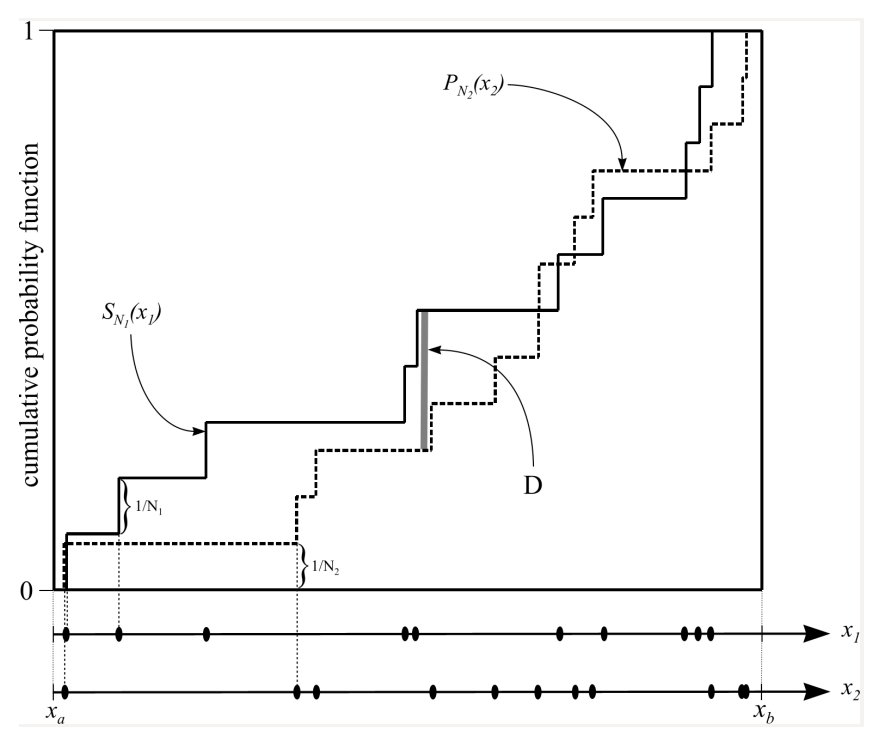
\includegraphics[height=6.9cm]{ks.eps}
   \caption{The Kolmogorov-Smirnov test}
\end{figure}
%-----------------------------------------------------------
Here an example for the way of constructing a CDF: Assume there
are $N_1=10$ measurements within a range of $[x_a,x_b]$. The data
points are shown as the quantity $x_1$ on the line labelled $x_1$
at the bottom of Fig. B.1. The cumulative distribution function
$S_{N_1}(x_1)$ is constructed by starting at $x_a$ and `moving' to
$x_b$. On every data point of $x_1$ the CDF is increased by
$1/N_1$, so it cumulates from 0 to 1 when going from $x_a$ to
$x_b$. The result is a step function. The CDF value is constant
between data points. The same is done with the theoretical
distribution $P_{N_2}(x_2)$ the data of which are shown on the
line labelled $x_2$ at the bottom of Fig. B.1. In our case
$P_{N_2}(x_2)$ is based on random distributions of $10^6$
galaxies, so it has discrete values, too. This leads to a second
step function. However it is much more smoother than the one of
the observations, because of the higher number of data.\\\\
The K-S test behaves conservative in case of a discrete
$P_{N_2}(x_2)$, so it overestimates the null hypothesis. If
$P_{N_2}(x_2)$ is based on a continuous function, this test does
not overestimate the null hypothesis.\\\\
All cumulative functions constructed in this way have two common
properties: they are zero at the beginning of their range of
definition and 1 on their end. The comparison of the two
distribution functions $S_{N_1}(x_1)$ and a continuous theoretical
$P(x)$ is done with the help of the quantity $D$, which is defined
as
%--------------------------------------
\begin{equation}
    D=\max_{x_a<x<x_b}|S_{N_1}(x)-P(x)|
\end{equation}
%--------------------------------------
So it is the largest difference between the two cumulative
functions. In case of a non-continuous $P_{N_2}(x_2)$, as used in
this work, this becomes
%--------------------------------------
\begin{equation}
    D=\max_{x_a<x<x_b}|S_{N_1}(x)-P_{N_2}(x_2)|
\end{equation}
%--------------------------------------
The quantile ($Q_{KS}$) is a function of $\lambda$ and can be
calculated by
%--------------------------------------
\begin{equation}\label{k_s}
    Q_{KS}(\lambda)=2\sum_{j=1}^\infty (-1)^{j-1}e^{-2j^2\lambda^2}
\end{equation}
%--------------------------------------
which is a monotonic function with the limiting values
%--------------------------------------
\begin{equation}
    Q_{KS}(0)=1, \quad Q_{KS}(\infty)=0
\end{equation}
%--------------------------------------
The parameter $D$ measures the maximum values of the absolute
difference between two cumulative distribution functions. In terms
of this function, the significance level of an observed value of
$D$ is given approximately (Stephens 1970) by,
%---------------------------------------
\begin{equation}
    P(D>$observed$)=Q_{KS}([\sqrt{N_e}+0.12+0.11/\sqrt{N_e}]D)
\end{equation}
%---------------------------------------
where $N_e$ is the effective number of data points, defined by
%--------------------------------------
\begin{equation}
    N_e=\frac{N_1N_2}{N_1+N_2}.
\end{equation}
%--------------------------------------
with $N_1$ denoting the number of data in the observations and
$N_2$ being the number of data in the theoretical set.\\\\
The nature of the distribution given in equation \eqref{k_s} is that it
becomes asymptotically accurate as the $N_e$ becomes $\geq$ 4
(Stephens 1970).\\\\
The K-S test tends to be most sensitive around $P(x)=0.5$, the
median value. At $P(x)=0$ or 1 it is less sensitive. The reason is
that the probability for larger $D$ is largest at the median value
of $P(x)$, because at $P(x)=0$ and $P(x)=1$ both CDFs coincide,
whereas the probability of a coincidence is smallest at the median
value of $P(x)$. So a large amount of steps in one of the CDFs can
cause a larger distance between both CDFs around $P(x)=0.5$.\\\\
\section{Kuiper-V Test}\label{kvtest}
The Kuiper-$V$ statistics (Kuiper, 1962) is a variant of the
Kolmogorov-Smirnov statistics. The basic idea is to take advantage
of the invariance of reparametrization of the $x$-axis. One can
``wrap" the $x$-axis into a circle  and look
for a statistic which is invariant under shifts.
\begin{figure}[h]\label{kv}
   \centering
   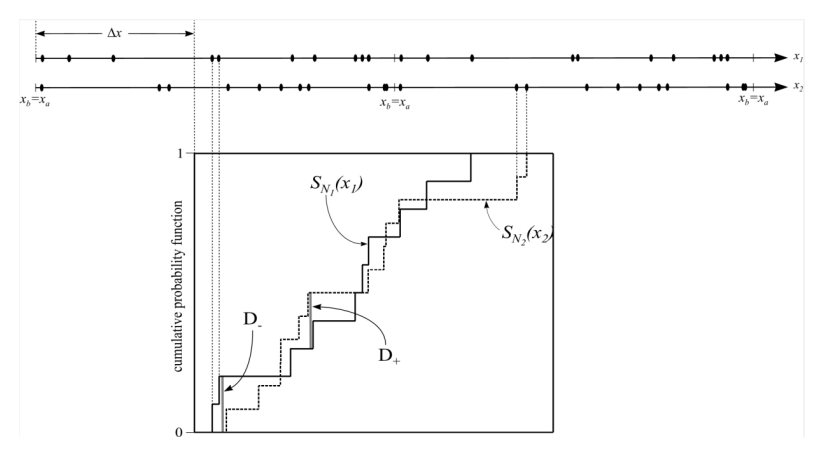
\includegraphics[height=9cm]{kuiper.eps}
   \caption{Kuiper-$V$ test: The CDF's are
   constructed in the same way like the K-S test, except the starting
   point is shifted by $\Delta x$ which leads to different CDF's. The measurement
   quantity for the Kuiper-$V$ test is the now the sum $D=D_++D_-$, the two largest
   distances above and below $S_{N_1}(x_1)$ between the two CDF's. This new quantity leads to an independence of
   the sensitivity of the test.}
\end{figure}
%----------------------------------------
The data set is the same as used in the example of the previous
chapter. Fig. B.2 shows the cumulative distribution functions
$S_{N_1}(x_1)$ and $S_{N_2}(x_2)$. It can be seen that they are
different from the one in Fig. B.1. The reason is that the starting
point is shifted by an offset $\Delta x$. The Kuiper-$V$
statistics is defined by
%--------------------------------------
\begin{equation}
\begin{array}{l}
    V=D_++D_-
    \\=\max[S_{N_1}(x)-S_{N_2}(x)]+\max[S_{N_2}(x)-S_{N_1}(x)]
\end{array}
\end{equation}
%--------------------------------------
$D_+$ and $D_-$ are the largest distances between $S_{N_1}$ and
$S_{N_2}$. $D_+$ lies above $S_{N_1}$, $D_-$ below.

The quantile ($Q_{KP}$) of the Kuiper-$V$-statistics can be
calculated by
%----------------------------------------
\begin{equation}
    Q_{KP}(\lambda)=2\sum_{j=1}^{\infty}(4j^2\lambda^2-1)e^{-2j^2\lambda^2}
\end{equation}
%----------------------------------------
which is again monotonic and has the following limits:
%----------------------------------------
\begin{equation}
    Q_{KP}(0)=1, \quad Q_{KP}(\infty)=0
\end{equation}
%----------------------------------------
The approximative function to calculate the significance level for
the disproof of the null hypothesis is given by (Stephens 1970)
%---------------------------------------
\begin{equation}
    P(V>$observed$)=Q_{KP}([\sqrt{N_e}+0.155+0.24/\sqrt{N_e}]V)
\end{equation}
%---------------------------------------
where $N_e$ represents the effective number of data points.\\\\
The trick to obtain the same sensitivity over the whole range of
definition is to take the sum of $D_+$ and $D_-$. So this
statistic becomes invariant under shifts (=variations of $\Delta
x$) (Kuiper, 1962). Therefore the sensitivity of the test is not a
function of $x$. Of course the individual values of $D_+$ and
$D_-$ vary with different starting points $\Delta x$, but the sum
stays constant (Kuiper, 1962). This property makes this test
perfect for all problems defined on circles, periods, cycles, and
so on.\\\\
The conditions for anisotropy are as follows:
chi-square probability P($>\chi^2)<$0.050, correlation
coefficient $C/\sigma(C)>$1, first order Fourier coefficient
$\Delta_{11}$/$\sigma(\Delta_{11}$)$>$1 and the first order
Fourier probability P($>\Delta_1$)$>$0.150 as used by Godlowski
(1993, 1994) K-S=1 and Kuiper-V=1. In $\theta$ distribution, a positive(negative) $\Delta_{11}$ suggests that the spin vectors of galxies tend to orient parallel  (perpendicular) to the reference coordinate system. In $\phi$-distribution, a postive (negative) $\Delta_{11}$ suggests that the spin vector projections of galaxies tend to point radially (tangentially) with respect to center of the reference coordinate system.


\chapter{Holmberg Equation}\label{holm}
Erik Holmberg (1946) established a simple galaxy model which we have used in the study of spin vector alignment. The two major axes in the main plane are of equal size a, the polar axis is the smallest one denoting the relative thickness of the ellipsoid. It has lenght $q\,a$, $q$ being the so called flatness factor, a number $\in$ [0,1] corresponding to the relative thickness of real spiral galaxies. Holmberg (1946) suggested a value of $q$= 0.2.
\section{Relation Between The Inclination And The Axial Ratio}
Holmberg equation is the relation between the axial ratio, $\frac{b}{a}$ and the inclination angle $i$, angle measured between the line-of-sight and direction perpendicular to the plane defined by the two major semi axes.
\begin{figure}
\centering
	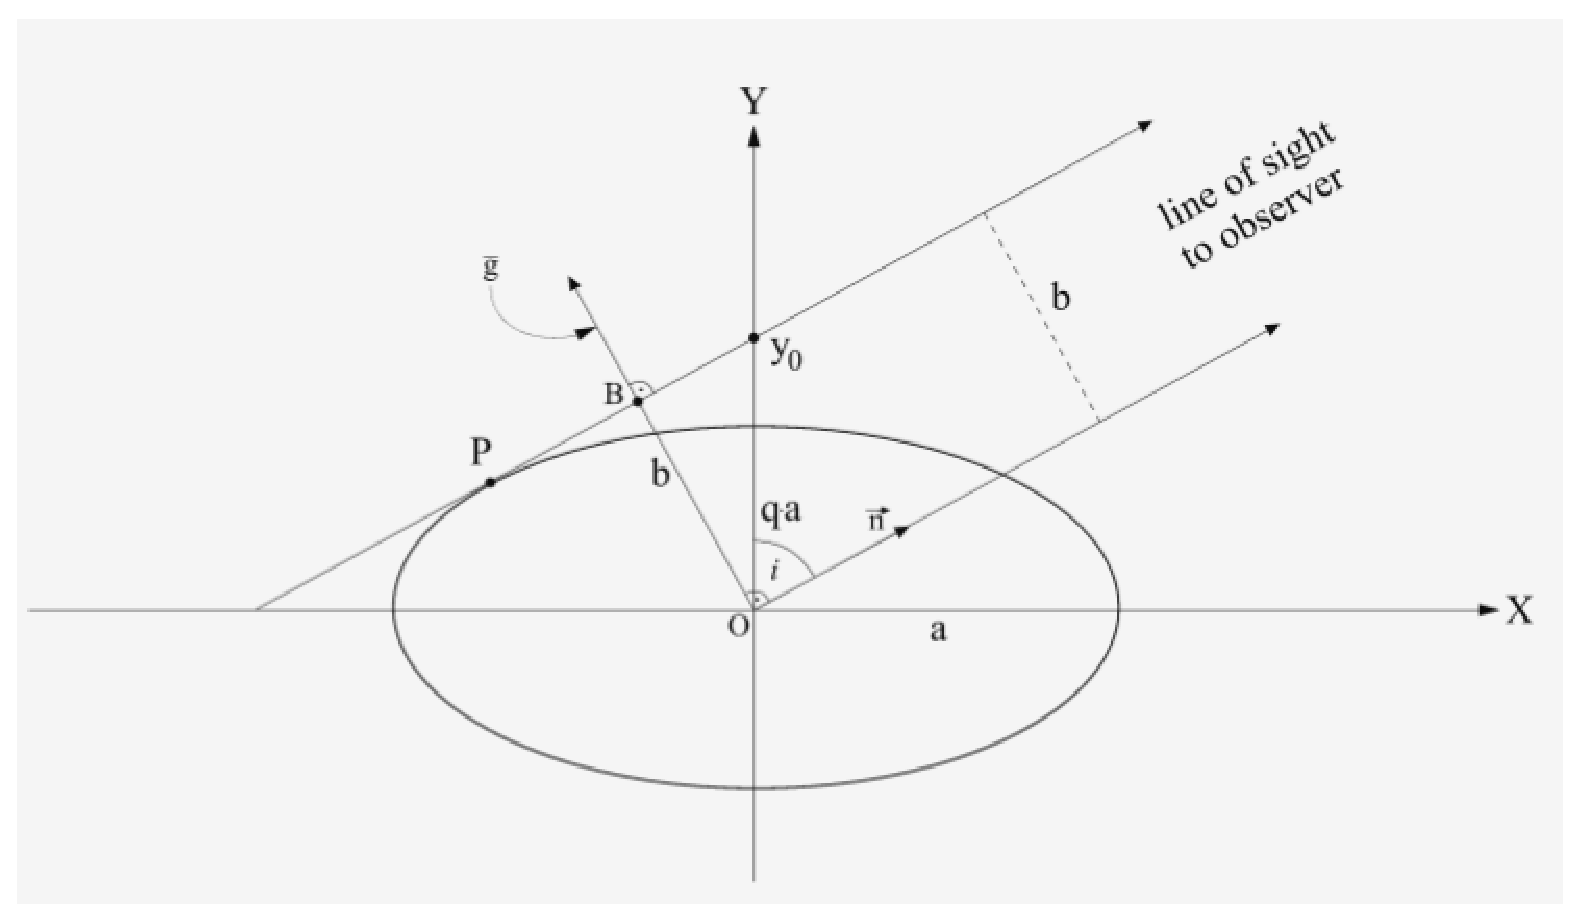
\includegraphics[height=6cm]{hom.eps}
	\caption{Derivation of Holmberg equation. (Hubble E. 1926)}\label{hom}
\end{figure}
Fig \ref{hom} shows the oblate spheroid aside, so an ellipse with an eccentricity of 0.2 is drawn. The celestial plane is perpendicular to the paper plane, intersection line is denoted by $\bar{g}$.\\\\
Fig \ref{hom} also shows the line of sight to the observer, the inclination $i$ is measured between this line and the Y-axis. This angle can be found between $\bar{g}$ and the -X-direction.\\\\
The equation of the ellipse is
\begin{equation}\label{ellipse}
q^2\,x^2 + y^2 = a^2\,q^2
\end{equation}
From the observers point of view the oblate spheroid seems to be projected onto the celestial plane as an ellipse. The quantity b, the connecting line $\bar{OB}$, is the small semi axis of this ellipse, the large semi axis $a$ of which is independent of the projection, so it is same as the one of oblate spheroid.\\\\
Assume a tangent in point $P$. The equation of the tangent is \begin{equation}\label{tangent}y=k\,x + y_0\end{equation}The condition for contact to the ellipse in Fig \ref{hom} is determined by applying the condition that \eqref{ellipse} and \eqref{tangent} touches each other. i.e 
\begin{equation}
a^2\,k^2 + a^2\,q^2 = y_0^2
\end{equation}
beging $k\,=\,cot\,i$ the slope of the tangent and $y_0$ the intersection of the tangent wiht the Y-axis.\\\\
This can be used to determine $y_0:$
\begin{equation}\label{red_cond}
y_0^2 = a^2 \cot^2\,i + a^2\,q^2
\end{equation} 
Using $b=y_0\,\sin\,i$ in \eqref{red_cond} we get
\begin{equation}
\sin^2 i=\frac{\frac{b^2}{a^2}-1}{q^2-1}
\end{equation}
which leads to
\begin{equation}\label{holmberg_equation}
\cos^2 i=\frac{\frac{b^2}{a^2}-q^2}{1-q^2}
\end{equation}
\eqref{holmberg_equation} is called \textquoteleft Holmberg Formula\textquoteright. It can be seen that there is a strong nonlinearity at large diameter ratios. The small measurement errors in teh semiaxes produce large deviations in the resulting inclinaiton angle.
\begin{figure}[H]
\begin{center}
\includegraphics[height=6cm]{holmberg.eps}
\end{center}
\caption{Plot of the Holmberg Function: There is a strong nonlinearity at the lower
and the upper end of the diameter ratio interval. The flatness factor q = 0.2}
\end{figure}
\chapter{Distribution of inclination angle $i$, longitude $L$ and latitude $B$}
\section{Transformation of Random Distribution}
If $x_1$, $x_2$ ,$x_3$, $\ldots$ are the random deviates with a joint probablity distribution $p(x_1,x_2,x_3,\ldots)$ and if $y_1$, $y_2$, $y_3$,$\ldots\ldots$ are each function of all $x$, then the joint probablity distribution of the $y$ is given by:
\begin{equation}\label{prob_dist}
p(y_1,y_2,y_3,\ldots)dy_1dy_2dy_3\ldots = p(x_1,x_2,x_3,\ldots)\left|\frac{\partial(x_1,x_2,x_3,\ldots)}{\partial(y_1,y_2,y_3,\ldots)}\right|dy_1dy_2dy_3\ldots
\end{equation} 
where $|\partial()/\partial()|$ is the Jacobian of the $x$ with respect to the $y$ (or reciprocal of the Jacobian determinant of the $y$ with respect to the $x$).
\subsection{Random Distribution to Spherical Random Distribution}
Let us consider uniform random distribution of the points in a sphere. Now we have to determine the distribution of the points with respect to the spherical coordinates i.e radius $r$, polar angle $\theta$ and azimuthal angle $\phi$. Then,
\begin{equation}\label{transformation}
\begin{aligned}
x=r\cos\phi\sin\theta\\
y=r\sin\phi\sin\theta\\
z=r\cos\theta
\end{aligned}
\end{equation}

And the Jacobian for transfomation given in \eqref{transformation} is $r^2\,\sin\theta$.
So from \eqref{prob_dist} we have
\begin{equation}\label{prob}
p(r,\theta,\phi)dr\,d\theta\,d\phi=r^2sin\theta\,p(x,y,z)dr\,d\theta\,d\phi
\end{equation}
From \eqref{prob}, if the probablity distribution in r, $\theta$ and $\phi$ are independent and similar case for $x\,\,y\,\,z$ we can write
\begin{equation}
p(r) p(\theta) p(\phi) = r^2 \sin\theta p(x) p(y) p(z)
\end{equation}
But $p(x)=p(y)=p(z)=1$. So,
\begin{equation}
\begin{aligned}
p(r)&=&r^2\\p(\theta)&=&\sin\theta\\p(\phi)&=&1
\end{aligned}
\end{equation} 
From above we can say that the $\theta$ distribution is $\sin\theta$ and $\phi$ is uniformly randomly distributed.
\section{Distribution of $B$ and $L$}
If we make analogy with the spherical coordinates, we can easily see that $B$ = $\frac{\pi}{2}-\theta$ and $L$ = $\phi$. The distribution of the galaxies are uniformly random in the surface of celestial sphere. So, we can deduce that the distribution of $B$ is $\sin(\frac{\pi}{2}-B)=\cos B$ and the distribution of $L$ is uniform.

\section{Distribution of inclination angle $i$}
If we consider line of sight as the Z-axis and make analogy with the spherical coordinates then $i$ = $\theta$. As we consider the distribution of galaxies to be isotropic so the distribution of inclination angle $i$ is $\sin i$.
\include{appendixe}
\end{appendix}
}
%-----------------------------------------------------------
\end{document}
